% **************************************************************************************************************
% A Classic Thesis Style
% An Homage to The Elements of Typographic Style
%
% Copyright (C) 2015 André Miede http://www.miede.de
%
% If you like the style then I would appreciate a postcard. My address 
% can be found in the file ClassicThesis.pdf. A collection of the 
% postcards I received so far is available online at 
% http://postcards.miede.de
%
% License:
% This program is free software; you can redistribute it and/or modify
% it under the terms of the GNU General Public License as published by
% the Free Software Foundation; either version 2 of the License, or
% (at your option) any later version.
%
% This program is distributed in the hope that it will be useful,
% but WITHOUT ANY WARRANTY; without even the implied warranty of
% MERCHANTABILITY or FITNESS FOR A PARTICULAR PURPOSE.  See the
% GNU General Public License for more details.
%
% You should have received a copy of the GNU General Public License
% along with this program; see the file COPYING.  If not, write to
% the Free Software Foundation, Inc., 59 Temple Place - Suite 330,
% Boston, MA 02111-1307, USA.
%
% **************************************************************************************************************
\RequirePackage{fix-cm} % fix some latex issues see: http://texdoc.net/texmf-dist/doc/latex/base/fixltx2e.pdf
\documentclass[ twoside,openright,titlepage,numbers=noenddot,headinclude,%1headlines,% letterpaper a4paper
                footinclude=true,cleardoublepage=empty,abstractoff, % <--- obsolete, remove (todo)
                BCOR=5mm,paper=a4,fontsize=11pt,%11pt,a4paper,%
                ngerman,american,%
                ]{scrreprt}

%********************************************************************
% Note: Make all your adjustments in here
%*******************************************************
% ****************************************************************************************************
% classicthesis-config.tex 
% formerly known as loadpackages.sty, classicthesis-ldpkg.sty, and classicthesis-preamble.sty 
% Use it at the beginning of your ClassicThesis.tex, or as a LaTeX Preamble 
% in your ClassicThesis.{tex,lyx} with % ****************************************************************************************************
% classicthesis-config.tex 
% formerly known as loadpackages.sty, classicthesis-ldpkg.sty, and classicthesis-preamble.sty 
% Use it at the beginning of your ClassicThesis.tex, or as a LaTeX Preamble 
% in your ClassicThesis.{tex,lyx} with % ****************************************************************************************************
% classicthesis-config.tex 
% formerly known as loadpackages.sty, classicthesis-ldpkg.sty, and classicthesis-preamble.sty 
% Use it at the beginning of your ClassicThesis.tex, or as a LaTeX Preamble 
% in your ClassicThesis.{tex,lyx} with \input{classicthesis-config}
% ****************************************************************************************************  
% If you like the classicthesis, then I would appreciate a postcard. 
% My address can be found in the file ClassicThesis.pdf. A collection 
% of the postcards I received so far is available online at 
% http://postcards.miede.de
% ****************************************************************************************************


% ****************************************************************************************************
% 0. Set the encoding of your files. UTF-8 is the only sensible encoding nowadays. If you can't read
% äöüßáéçèê∂åëæƒÏ€ then change the encoding setting in your editor, not the line below. If your editor
% does not support utf8 use another editor!
% ****************************************************************************************************
\PassOptionsToPackage{utf8}{inputenc}
\usepackage{inputenc}
        
% ****************************************************************************************************
% 1. Configure classicthesis for your needs here, e.g., remove "drafting" below 
% in order to deactivate the time-stamp on the pages
% ****************************************************************************************************
\PassOptionsToPackage{eulerchapternumbers,listings,%drafting,%
					 pdfspacing,%floatperchapter,%linedheaders,%
					 subfig,beramono,eulermath,parts}{classicthesis}                                        
% ********************************************************************
% Available options for classicthesis.sty 
% (see ClassicThesis.pdf for more information):
% drafting
% parts nochapters linedheaders
% eulerchapternumbers beramono eulermath pdfspacing minionprospacing
% tocaligned dottedtoc manychapters
% listings floatperchapter subfig
% ********************************************************************

\usepackage{url}
\usepackage{nameref}
\usepackage{datetime} %needed to add the date just below
% ****************************************************************************************************
% 2. Personal data and user ad-hoc commands
% ****************************************************************************************************
\newcommand{\myTitle}{Utilizing IPFS as content provider for DASH video streaming\xspace}
\newcommand{\mySubtitle}{Evaluating UX and performance of DASH streaming with decentralized video content delivered through IPFS\xspace}
\newcommand{\myDegree}{Master's Thesis\xspace}
\newcommand{\myName}{Andreas Østergaard Nielsen\xspace}
\newcommand{\myStudentId}{201303609\xspace}
\newcommand{\myOtherName}{Andreas Malling Østergaard\xspace}
\newcommand{\myOtherStudentId}{201303553\xspace}
\newcommand{\myProf}{Niels Olof Bouvin\xspace}
\newcommand{\myOtherProf}{Put name here\xspace}
\newcommand{\mySupervisor}{Put name here\xspace}
\newcommand{\myFaculty}{Science \& Technology\xspace}
\newcommand{\myDepartment}{Department of Computer Science\xspace}
\newcommand{\myUni}{Aarhus University\xspace}
\newcommand{\myLocation}{Aarhus\xspace}
\newcommand{\myTime}{\monthname\ \the\year\xspace}
\newcommand{\myVersion}{massive edition\xspace}


% ********************************************************************
% Setup, finetuning, and useful commands
% ********************************************************************
\newcounter{dummy} % necessary for correct hyperlinks (to index, bib, etc.)
\newlength{\abcd} % for ab..z string length calculation
\providecommand{\mLyX}{L\kern-.1667em\lower.25em\hbox{Y}\kern-.125emX\@}
% \newcommand{\ie}{i.\,e.}
% \newcommand{\Ie}{I.\,e.}
% \newcommand{\eg}{e.\,g.}
% \newcommand{\Eg}{E.\,g.} 
% ****************************************************************************************************


% ****************************************************************************************************
% 3. Loading some handy packages
% ****************************************************************************************************
% ******************************************************************** 
% Packages with options that might require adjustments
% ******************************************************************** 
%\PassOptionsToPackage{ngerman,american}{babel}   % change this to your language(s)
% Spanish languages need extra options in order to work with this template
%\PassOptionsToPackage{spanish,es-lcroman}{babel}
\usepackage[american]{babel}                  
\usepackage{microtype}
\usepackage{csquotes}
\usepackage{ragged2e}
\usepackage[dvipsnames, table]{xcolor}
\usepackage{pgf-umlsd}
\usepackage{pgfplots}
\usepackage{pgfplotstable}
\pgfplotsset{compat=1.15}
\usepackage{tikz}

% recommended:
\usepackage{booktabs}
\usepackage{array}
\usepackage{colortbl}
% \usepackage{color}

\definecolor{dkgreen}{rgb}{0,0.6,0}
\definecolor{gray}{rgb}{0.5,0.5,0.5}
\definecolor{mauve}{rgb}{0.58,0,0.82}
\definecolor{gray}{rgb}{0.4,0.4,0.4}
\definecolor{darkblue}{rgb}{0.0,0.0,0.6}
\definecolor{lightblue}{rgb}{0.0,0.0,0.9}
\definecolor{cyan}{rgb}{0.0,0.6,0.6}
\definecolor{darkred}{rgb}{0.6,0.0,0.0}
\definecolor{lightyellow}{rgb}{1,1,0.85}

% custom:
\newcommand{\setexpid}[1] {\label{exp:#1}#1}

\newcommand{\expid}[1] {\hyperref[exp:#1]{Exp.ID #1}}

\usepackage{media9} % youtube video

\usepackage[section]{placeins}  % floatbarrier

%\usepackage[square,numbers,sort&compress]{natbib}
%\bibliographystyle{abbrvnat}

\PassOptionsToPackage{%
   %backend=biber, %instead of bibtex
	backend=bibtex8,bibencoding=ascii,%
	language=auto,%
	style=numeric-comp,%
   %style=authoryear-comp, % Author 1999, 2010
   %bibstyle=authoryear,dashed=false, % dashed: substitute rep. author with ---
   sorting=nyt, % name, year, title
   maxbibnames=10, % default: 3, et al.
   maxcitenames=2,
   %backref=true,%
   natbib=true % natbib compatibility mode (\citep and \citet still work)
}{biblatex}
\usepackage{biblatex}

\PassOptionsToPackage{fleqn}{amsmath}       % math environments and more by the AMS 
\usepackage{amsmath}
%
% ******************************************************************** 
% General useful packages
% ******************************************************************** 
\PassOptionsToPackage{T1}{fontenc} % T2A for cyrillics
\usepackage{fontenc}     
\usepackage{textcomp} % fix warning with missing font shapes
\usepackage{scrhack} % fix warnings when using KOMA with listings package          
\usepackage{xspace} % to get the spacing after macros right  
\newcommand{\eg}{e.g.,\xspace}
\newcommand{\Eg}{E.g.,\xspace}
\newcommand{\etal}{et~al.\xspace}
\newcommand{\etc}{etc.\@\xspace}
\newcommand{\ie}{i.e.,\xspace}
\newcommand{\viz}{viz.\@\xspace}

\usepackage{mparhack} % get marginpar right
%\usepackage{fixltx2e} % fixes some LaTeX stuff --> since 2015 in the LaTeX kernel (see below)
%\usepackage[latest]{latexrelease} % will be used once available in more distributions (ISSUE #107)
\PassOptionsToPackage{printonlyused,smaller}{acronym} 
    \usepackage{acronym} % nice macros for handling all acronyms in the thesis
    %\renewcommand{\bflabel}[1]{{#1}\hfill} % fix the list of acronyms --> no longer working
    %\renewcommand*{\acsfont}[1]{\textsc{#1}} 
    \renewcommand*{\aclabelfont}[1]{\acsfont{#1}}
% ****************************************************************************************************


% ****************************************************************************************************
% 4. Setup floats: tables, (sub)figures, and captions
% ****************************************************************************************************
\usepackage{tabularx} % better tables
    \setlength{\extrarowheight}{3pt} % increase table row height
\newcommand{\tableheadline}[1]{\multicolumn{1}{c}{\spacedlowsmallcaps{#1}}}
\newcommand{\myfloatalign}{\centering} % to be used with each float for alignment
\usepackage{caption}
% Thanks to cgnieder and Claus Lahiri
% http://tex.stackexchange.com/questions/69349/spacedlowsmallcaps-in-caption-label
% [REMOVED DUE TO OTHER PROBLEMS, SEE ISSUE #82]    
%\DeclareCaptionLabelFormat{smallcaps}{\bothIfFirst{#1}{~}\MakeTextLowercase{\textsc{#2}}}
%\captionsetup{font=small,labelformat=smallcaps} % format=hang,
\captionsetup{font=small} % format=hang,
\usepackage{subfig}
\usepackage{multirow}


\newcommand{\repeatcaption}[2]{%
  \renewcommand{\thefigure}{\ref{#1}}%
  \captionsetup{list=no}%
  \caption{#2 (repeated from \autopageref{#1})}%
}

\newcommand{\rptcaption}[1]{%
  \renewcommand{\thefigure}{\ref{#1}}%
  \captionsetup{list=no}%
  \caption{\nameref*{#1} (repeated from \autopageref{#1})}%
}

% ****************************************************************************************************


% ****************************************************************************************************
% 5. Setup code listings
% ****************************************************************************************************
\usepackage[]{algorithm2e}
\usepackage{listings} 
%\lstset{emph={trueIndex,root},emphstyle=\color{BlueViolet}}%\underbar} % for special keywords
\lstset{language=[LaTeX]Tex,%C++,
    morekeywords={PassOptionsToPackage,selectlanguage},
    keywordstyle=\color{darkblue},%\bfseries,
    basicstyle=\small\ttfamily,
    identifierstyle=\color{NavyBlue},
    commentstyle=\color{Green}\ttfamily,
    stringstyle=\rmfamily,
    numbers=left,
    numberstyle=\tiny\color{Gray},
    stepnumber=1,
    numbersep=8pt,
    showstringspaces=false,
    breaklines=true,
    %frameround=ftff,
    %frame=single,
    belowcaptionskip=.75\baselineskip
    %frame=L
}

\lstdefinelanguage{MPD}
{
  morestring=[s][\color{mauve}]{"}{"},
  morestring=[s][\color{black}]{>}{<},
  morecomment=[s]{<?}{?>},
  morecomment=[s][\color{dkgreen}]{<!--}{-->},
  stringstyle=\color{black},
  identifierstyle=\color{lightblue},
  keywordstyle=\color{red},
  morekeywords={MPD,ProgramInformation,Title,Period,AdaptationSet,SegmentTemplate,Representation,AudioChannelConfiguration}% list your attributes here
}

\lstdefinelanguage{pseudo}{
    morekeywords={If, Else, For, In, Remove, From, Case, Do, While, False, True},
    sensitive=true,
    morecomment=[l]{\#},
    morecomment=[l]{//},
    morestring=[b]{'}
}

\lstdefinelanguage{env}{
  morecomment=[l]{\#},
  identifierstyle=\color{black},
  stringstyle=\color{black},
  morekeywords={SCALE_MONGO,SCALE_METRIC,SCALE_NETWORK,SCALE_HOST,SCALE_BOOT,SCALE_SEED,SCALE_USER_1,SCALE_USER_2,SCALE_USER_3,SCALE_USER_4,SCALE_USER_5,SCALE_USER_6,USER_1,USER_2,USER_3,USER_4,USER_5,USER_6}
  }
  
  \lstdefinelanguage{docker-compose}{
  keywords={version, services},
  keywordstyle=\color{blue}\bfseries,
  keywords=[2]{image, environment, ports, container_name, ports, links, build, depends_on, command, volumes},
  keywordstyle=[2]\color{orange}\bfseries,
  identifierstyle=\color{black},
  sensitive=false,
  comment=[l]{\#},
  commentstyle=\color{purple}\ttfamily,
  stringstyle=\color{red}\ttfamily,
  morestring=[b]',
  morestring=[b]"
}
% ****************************************************************************************************             


% ****************************************************************************************************
% 6. PDFLaTeX, hyperreferences and citation backreferences
% ****************************************************************************************************
% ********************************************************************
% Using PDFLaTeX
% ********************************************************************
\PassOptionsToPackage{pdftex,hyperfootnotes=false,pdfpagelabels}{hyperref}
    \usepackage{hyperref}  % backref linktocpage pagebackref
\pdfcompresslevel=9
\pdfadjustspacing=1 
\PassOptionsToPackage{pdftex}{graphicx}
    \usepackage{graphicx} 
\graphicspath{ {gfx/} }
\newcommand{\source}[1]{\vspace{-9pt}\caption*{\textit{Source:} {#1}} }

% ********************************************************************
% Hyperreferences
% ********************************************************************
\hypersetup{%
    %draft, % = no hyperlinking at all (useful in b/w printouts)
    colorlinks=true, linktocpage=true, pdfstartpage=3, pdfstartview=FitV,%
    % uncomment the following line if you want to have black links (e.g., for printing)
    %colorlinks=false, linktocpage=false, pdfstartpage=3, pdfstartview=FitV, pdfborder={0 0 0},%
    breaklinks=true, pdfpagemode=UseNone, pageanchor=true, pdfpagemode=UseOutlines,%
    plainpages=false, bookmarksnumbered, bookmarksopen=true, bookmarksopenlevel=1,%
    hypertexnames=true, pdfhighlight=/O,%nesting=true,%frenchlinks,%
    urlcolor=webbrown, linkcolor=RoyalBlue, citecolor=webgreen, %pagecolor=RoyalBlue,%
    %urlcolor=Black, linkcolor=Black, citecolor=Black, %pagecolor=Black,%
    pdftitle={\myTitle},%
    pdfauthor={\textcopyright\ \myName, \myUni, \myFaculty},%
    pdfsubject={},%
    pdfkeywords={},%
    pdfcreator={pdfLaTeX},%
    pdfproducer={LaTeX with hyperref and classicthesis}%
}   

% ********************************************************************
% Setup autoreferences
% ********************************************************************
% There are some issues regarding autorefnames
% http://www.ureader.de/msg/136221647.aspx
% http://www.tex.ac.uk/cgi-bin/texfaq2html?label=latexwords
% you have to redefine the makros for the 
% language you use, e.g., american, ngerman
% (as chosen when loading babel/AtBeginDocument)
% ********************************************************************
\makeatletter
\@ifpackageloaded{babel}%
    {%
       \addto\extrasamerican{%
			\renewcommand*{\figureautorefname}{Figure}%
			\renewcommand*{\tableautorefname}{Table}%
			\renewcommand*{\partautorefname}{Part}%
			\renewcommand*{\chapterautorefname}{Chapter}%
			\renewcommand*{\sectionautorefname}{Section}%
			\renewcommand*{\subsectionautorefname}{Section}%
			\renewcommand*{\subsubsectionautorefname}{Section}%     
                }%
       \addto\extrasngerman{% 
			\renewcommand*{\paragraphautorefname}{Absatz}%
			\renewcommand*{\subparagraphautorefname}{Unterabsatz}%
			\renewcommand*{\footnoteautorefname}{Fu\"snote}%
			\renewcommand*{\FancyVerbLineautorefname}{Zeile}%
			\renewcommand*{\theoremautorefname}{Theorem}%
			\renewcommand*{\appendixautorefname}{Anhang}%
			\renewcommand*{\equationautorefname}{Gleichung}%        
			\renewcommand*{\itemautorefname}{Punkt}%
                }%  
            % Fix to getting autorefs for subfigures right (thanks to Belinda Vogt for changing the definition)
            \providecommand{\subfigureautorefname}{\figureautorefname}%             
    }{\relax}
\makeatother


% ****************************************************************************************************
% 7. Last calls before the bar closes
% ****************************************************************************************************
% ********************************************************************
% Development Stuff
% ********************************************************************
\listfiles
%\PassOptionsToPackage{l2tabu,orthodox,abort}{nag}
%   \usepackage{nag}
%\PassOptionsToPackage{warning, all}{onlyamsmath}
%   \usepackage{onlyamsmath}

% ********************************************************************
% Last, but not least...
% ********************************************************************
\usepackage{classicthesis} 
% ****************************************************************************************************


% ****************************************************************************************************
% 8. Further adjustments (experimental)
% ****************************************************************************************************
% ********************************************************************
% Changing the text area
% ********************************************************************
%\linespread{1.05} % a bit more for Palatino
%\areaset[current]{312pt}{761pt} % 686 (factor 2.2) + 33 head + 42 head \the\footskip
%\setlength{\marginparwidth}{7em}%
%\setlength{\marginparsep}{2em}%

% ********************************************************************
% Using different fonts
% ********************************************************************
%\usepackage[oldstylenums]{kpfonts} % oldstyle notextcomp
%\usepackage[osf]{libertine}
%\usepackage[light,condensed,math]{iwona}
%\renewcommand{\sfdefault}{iwona}
%\usepackage{lmodern} % <-- no osf support :-(
%\usepackage{cfr-lm} % 
%\usepackage[urw-garamond]{mathdesign} <-- no osf support :-(
%\usepackage[default,osfigures]{opensans} % scale=0.95 
%\usepackage[sfdefault]{FiraSans}
% ****************************************************************************************************



%%% Local Variables:
%%% mode: latex
%%% TeX-master: "./ClassicThesis"
%%% End:

% ****************************************************************************************************  
% If you like the classicthesis, then I would appreciate a postcard. 
% My address can be found in the file ClassicThesis.pdf. A collection 
% of the postcards I received so far is available online at 
% http://postcards.miede.de
% ****************************************************************************************************


% ****************************************************************************************************
% 0. Set the encoding of your files. UTF-8 is the only sensible encoding nowadays. If you can't read
% äöüßáéçèê∂åëæƒÏ€ then change the encoding setting in your editor, not the line below. If your editor
% does not support utf8 use another editor!
% ****************************************************************************************************
\PassOptionsToPackage{utf8}{inputenc}
\usepackage{inputenc}
        
% ****************************************************************************************************
% 1. Configure classicthesis for your needs here, e.g., remove "drafting" below 
% in order to deactivate the time-stamp on the pages
% ****************************************************************************************************
\PassOptionsToPackage{eulerchapternumbers,listings,%drafting,%
					 pdfspacing,%floatperchapter,%linedheaders,%
					 subfig,beramono,eulermath,parts}{classicthesis}                                        
% ********************************************************************
% Available options for classicthesis.sty 
% (see ClassicThesis.pdf for more information):
% drafting
% parts nochapters linedheaders
% eulerchapternumbers beramono eulermath pdfspacing minionprospacing
% tocaligned dottedtoc manychapters
% listings floatperchapter subfig
% ********************************************************************

\usepackage{url}
\usepackage{nameref}
\usepackage{datetime} %needed to add the date just below
% ****************************************************************************************************
% 2. Personal data and user ad-hoc commands
% ****************************************************************************************************
\newcommand{\myTitle}{Utilizing IPFS as content provider for DASH video streaming\xspace}
\newcommand{\mySubtitle}{Evaluating UX and performance of DASH streaming with decentralized video content delivered through IPFS\xspace}
\newcommand{\myDegree}{Master's Thesis\xspace}
\newcommand{\myName}{Andreas Østergaard Nielsen\xspace}
\newcommand{\myStudentId}{201303609\xspace}
\newcommand{\myOtherName}{Andreas Malling Østergaard\xspace}
\newcommand{\myOtherStudentId}{201303553\xspace}
\newcommand{\myProf}{Niels Olof Bouvin\xspace}
\newcommand{\myOtherProf}{Put name here\xspace}
\newcommand{\mySupervisor}{Put name here\xspace}
\newcommand{\myFaculty}{Science \& Technology\xspace}
\newcommand{\myDepartment}{Department of Computer Science\xspace}
\newcommand{\myUni}{Aarhus University\xspace}
\newcommand{\myLocation}{Aarhus\xspace}
\newcommand{\myTime}{\monthname\ \the\year\xspace}
\newcommand{\myVersion}{massive edition\xspace}


% ********************************************************************
% Setup, finetuning, and useful commands
% ********************************************************************
\newcounter{dummy} % necessary for correct hyperlinks (to index, bib, etc.)
\newlength{\abcd} % for ab..z string length calculation
\providecommand{\mLyX}{L\kern-.1667em\lower.25em\hbox{Y}\kern-.125emX\@}
% \newcommand{\ie}{i.\,e.}
% \newcommand{\Ie}{I.\,e.}
% \newcommand{\eg}{e.\,g.}
% \newcommand{\Eg}{E.\,g.} 
% ****************************************************************************************************


% ****************************************************************************************************
% 3. Loading some handy packages
% ****************************************************************************************************
% ******************************************************************** 
% Packages with options that might require adjustments
% ******************************************************************** 
%\PassOptionsToPackage{ngerman,american}{babel}   % change this to your language(s)
% Spanish languages need extra options in order to work with this template
%\PassOptionsToPackage{spanish,es-lcroman}{babel}
\usepackage[american]{babel}                  
\usepackage{microtype}
\usepackage{csquotes}
\usepackage{ragged2e}
\usepackage[dvipsnames, table]{xcolor}
\usepackage{pgf-umlsd}
\usepackage{pgfplots}
\usepackage{pgfplotstable}
\pgfplotsset{compat=1.15}
\usepackage{tikz}

% recommended:
\usepackage{booktabs}
\usepackage{array}
\usepackage{colortbl}
% \usepackage{color}

\definecolor{dkgreen}{rgb}{0,0.6,0}
\definecolor{gray}{rgb}{0.5,0.5,0.5}
\definecolor{mauve}{rgb}{0.58,0,0.82}
\definecolor{gray}{rgb}{0.4,0.4,0.4}
\definecolor{darkblue}{rgb}{0.0,0.0,0.6}
\definecolor{lightblue}{rgb}{0.0,0.0,0.9}
\definecolor{cyan}{rgb}{0.0,0.6,0.6}
\definecolor{darkred}{rgb}{0.6,0.0,0.0}
\definecolor{lightyellow}{rgb}{1,1,0.85}

% custom:
\newcommand{\setexpid}[1] {\label{exp:#1}#1}

\newcommand{\expid}[1] {\hyperref[exp:#1]{Exp.ID #1}}

\usepackage{media9} % youtube video

\usepackage[section]{placeins}  % floatbarrier

%\usepackage[square,numbers,sort&compress]{natbib}
%\bibliographystyle{abbrvnat}

\PassOptionsToPackage{%
   %backend=biber, %instead of bibtex
	backend=bibtex8,bibencoding=ascii,%
	language=auto,%
	style=numeric-comp,%
   %style=authoryear-comp, % Author 1999, 2010
   %bibstyle=authoryear,dashed=false, % dashed: substitute rep. author with ---
   sorting=nyt, % name, year, title
   maxbibnames=10, % default: 3, et al.
   maxcitenames=2,
   %backref=true,%
   natbib=true % natbib compatibility mode (\citep and \citet still work)
}{biblatex}
\usepackage{biblatex}

\PassOptionsToPackage{fleqn}{amsmath}       % math environments and more by the AMS 
\usepackage{amsmath}
%
% ******************************************************************** 
% General useful packages
% ******************************************************************** 
\PassOptionsToPackage{T1}{fontenc} % T2A for cyrillics
\usepackage{fontenc}     
\usepackage{textcomp} % fix warning with missing font shapes
\usepackage{scrhack} % fix warnings when using KOMA with listings package          
\usepackage{xspace} % to get the spacing after macros right  
\newcommand{\eg}{e.g.,\xspace}
\newcommand{\Eg}{E.g.,\xspace}
\newcommand{\etal}{et~al.\xspace}
\newcommand{\etc}{etc.\@\xspace}
\newcommand{\ie}{i.e.,\xspace}
\newcommand{\viz}{viz.\@\xspace}

\usepackage{mparhack} % get marginpar right
%\usepackage{fixltx2e} % fixes some LaTeX stuff --> since 2015 in the LaTeX kernel (see below)
%\usepackage[latest]{latexrelease} % will be used once available in more distributions (ISSUE #107)
\PassOptionsToPackage{printonlyused,smaller}{acronym} 
    \usepackage{acronym} % nice macros for handling all acronyms in the thesis
    %\renewcommand{\bflabel}[1]{{#1}\hfill} % fix the list of acronyms --> no longer working
    %\renewcommand*{\acsfont}[1]{\textsc{#1}} 
    \renewcommand*{\aclabelfont}[1]{\acsfont{#1}}
% ****************************************************************************************************


% ****************************************************************************************************
% 4. Setup floats: tables, (sub)figures, and captions
% ****************************************************************************************************
\usepackage{tabularx} % better tables
    \setlength{\extrarowheight}{3pt} % increase table row height
\newcommand{\tableheadline}[1]{\multicolumn{1}{c}{\spacedlowsmallcaps{#1}}}
\newcommand{\myfloatalign}{\centering} % to be used with each float for alignment
\usepackage{caption}
% Thanks to cgnieder and Claus Lahiri
% http://tex.stackexchange.com/questions/69349/spacedlowsmallcaps-in-caption-label
% [REMOVED DUE TO OTHER PROBLEMS, SEE ISSUE #82]    
%\DeclareCaptionLabelFormat{smallcaps}{\bothIfFirst{#1}{~}\MakeTextLowercase{\textsc{#2}}}
%\captionsetup{font=small,labelformat=smallcaps} % format=hang,
\captionsetup{font=small} % format=hang,
\usepackage{subfig}
\usepackage{multirow}


\newcommand{\repeatcaption}[2]{%
  \renewcommand{\thefigure}{\ref{#1}}%
  \captionsetup{list=no}%
  \caption{#2 (repeated from \autopageref{#1})}%
}

\newcommand{\rptcaption}[1]{%
  \renewcommand{\thefigure}{\ref{#1}}%
  \captionsetup{list=no}%
  \caption{\nameref*{#1} (repeated from \autopageref{#1})}%
}

% ****************************************************************************************************


% ****************************************************************************************************
% 5. Setup code listings
% ****************************************************************************************************
\usepackage[]{algorithm2e}
\usepackage{listings} 
%\lstset{emph={trueIndex,root},emphstyle=\color{BlueViolet}}%\underbar} % for special keywords
\lstset{language=[LaTeX]Tex,%C++,
    morekeywords={PassOptionsToPackage,selectlanguage},
    keywordstyle=\color{darkblue},%\bfseries,
    basicstyle=\small\ttfamily,
    identifierstyle=\color{NavyBlue},
    commentstyle=\color{Green}\ttfamily,
    stringstyle=\rmfamily,
    numbers=left,
    numberstyle=\tiny\color{Gray},
    stepnumber=1,
    numbersep=8pt,
    showstringspaces=false,
    breaklines=true,
    %frameround=ftff,
    %frame=single,
    belowcaptionskip=.75\baselineskip
    %frame=L
}

\lstdefinelanguage{MPD}
{
  morestring=[s][\color{mauve}]{"}{"},
  morestring=[s][\color{black}]{>}{<},
  morecomment=[s]{<?}{?>},
  morecomment=[s][\color{dkgreen}]{<!--}{-->},
  stringstyle=\color{black},
  identifierstyle=\color{lightblue},
  keywordstyle=\color{red},
  morekeywords={MPD,ProgramInformation,Title,Period,AdaptationSet,SegmentTemplate,Representation,AudioChannelConfiguration}% list your attributes here
}

\lstdefinelanguage{pseudo}{
    morekeywords={If, Else, For, In, Remove, From, Case, Do, While, False, True},
    sensitive=true,
    morecomment=[l]{\#},
    morecomment=[l]{//},
    morestring=[b]{'}
}

\lstdefinelanguage{env}{
  morecomment=[l]{\#},
  identifierstyle=\color{black},
  stringstyle=\color{black},
  morekeywords={SCALE_MONGO,SCALE_METRIC,SCALE_NETWORK,SCALE_HOST,SCALE_BOOT,SCALE_SEED,SCALE_USER_1,SCALE_USER_2,SCALE_USER_3,SCALE_USER_4,SCALE_USER_5,SCALE_USER_6,USER_1,USER_2,USER_3,USER_4,USER_5,USER_6}
  }
  
  \lstdefinelanguage{docker-compose}{
  keywords={version, services},
  keywordstyle=\color{blue}\bfseries,
  keywords=[2]{image, environment, ports, container_name, ports, links, build, depends_on, command, volumes},
  keywordstyle=[2]\color{orange}\bfseries,
  identifierstyle=\color{black},
  sensitive=false,
  comment=[l]{\#},
  commentstyle=\color{purple}\ttfamily,
  stringstyle=\color{red}\ttfamily,
  morestring=[b]',
  morestring=[b]"
}
% ****************************************************************************************************             


% ****************************************************************************************************
% 6. PDFLaTeX, hyperreferences and citation backreferences
% ****************************************************************************************************
% ********************************************************************
% Using PDFLaTeX
% ********************************************************************
\PassOptionsToPackage{pdftex,hyperfootnotes=false,pdfpagelabels}{hyperref}
    \usepackage{hyperref}  % backref linktocpage pagebackref
\pdfcompresslevel=9
\pdfadjustspacing=1 
\PassOptionsToPackage{pdftex}{graphicx}
    \usepackage{graphicx} 
\graphicspath{ {gfx/} }
\newcommand{\source}[1]{\vspace{-9pt}\caption*{\textit{Source:} {#1}} }

% ********************************************************************
% Hyperreferences
% ********************************************************************
\hypersetup{%
    %draft, % = no hyperlinking at all (useful in b/w printouts)
    colorlinks=true, linktocpage=true, pdfstartpage=3, pdfstartview=FitV,%
    % uncomment the following line if you want to have black links (e.g., for printing)
    %colorlinks=false, linktocpage=false, pdfstartpage=3, pdfstartview=FitV, pdfborder={0 0 0},%
    breaklinks=true, pdfpagemode=UseNone, pageanchor=true, pdfpagemode=UseOutlines,%
    plainpages=false, bookmarksnumbered, bookmarksopen=true, bookmarksopenlevel=1,%
    hypertexnames=true, pdfhighlight=/O,%nesting=true,%frenchlinks,%
    urlcolor=webbrown, linkcolor=RoyalBlue, citecolor=webgreen, %pagecolor=RoyalBlue,%
    %urlcolor=Black, linkcolor=Black, citecolor=Black, %pagecolor=Black,%
    pdftitle={\myTitle},%
    pdfauthor={\textcopyright\ \myName, \myUni, \myFaculty},%
    pdfsubject={},%
    pdfkeywords={},%
    pdfcreator={pdfLaTeX},%
    pdfproducer={LaTeX with hyperref and classicthesis}%
}   

% ********************************************************************
% Setup autoreferences
% ********************************************************************
% There are some issues regarding autorefnames
% http://www.ureader.de/msg/136221647.aspx
% http://www.tex.ac.uk/cgi-bin/texfaq2html?label=latexwords
% you have to redefine the makros for the 
% language you use, e.g., american, ngerman
% (as chosen when loading babel/AtBeginDocument)
% ********************************************************************
\makeatletter
\@ifpackageloaded{babel}%
    {%
       \addto\extrasamerican{%
			\renewcommand*{\figureautorefname}{Figure}%
			\renewcommand*{\tableautorefname}{Table}%
			\renewcommand*{\partautorefname}{Part}%
			\renewcommand*{\chapterautorefname}{Chapter}%
			\renewcommand*{\sectionautorefname}{Section}%
			\renewcommand*{\subsectionautorefname}{Section}%
			\renewcommand*{\subsubsectionautorefname}{Section}%     
                }%
       \addto\extrasngerman{% 
			\renewcommand*{\paragraphautorefname}{Absatz}%
			\renewcommand*{\subparagraphautorefname}{Unterabsatz}%
			\renewcommand*{\footnoteautorefname}{Fu\"snote}%
			\renewcommand*{\FancyVerbLineautorefname}{Zeile}%
			\renewcommand*{\theoremautorefname}{Theorem}%
			\renewcommand*{\appendixautorefname}{Anhang}%
			\renewcommand*{\equationautorefname}{Gleichung}%        
			\renewcommand*{\itemautorefname}{Punkt}%
                }%  
            % Fix to getting autorefs for subfigures right (thanks to Belinda Vogt for changing the definition)
            \providecommand{\subfigureautorefname}{\figureautorefname}%             
    }{\relax}
\makeatother


% ****************************************************************************************************
% 7. Last calls before the bar closes
% ****************************************************************************************************
% ********************************************************************
% Development Stuff
% ********************************************************************
\listfiles
%\PassOptionsToPackage{l2tabu,orthodox,abort}{nag}
%   \usepackage{nag}
%\PassOptionsToPackage{warning, all}{onlyamsmath}
%   \usepackage{onlyamsmath}

% ********************************************************************
% Last, but not least...
% ********************************************************************
\usepackage{classicthesis} 
% ****************************************************************************************************


% ****************************************************************************************************
% 8. Further adjustments (experimental)
% ****************************************************************************************************
% ********************************************************************
% Changing the text area
% ********************************************************************
%\linespread{1.05} % a bit more for Palatino
%\areaset[current]{312pt}{761pt} % 686 (factor 2.2) + 33 head + 42 head \the\footskip
%\setlength{\marginparwidth}{7em}%
%\setlength{\marginparsep}{2em}%

% ********************************************************************
% Using different fonts
% ********************************************************************
%\usepackage[oldstylenums]{kpfonts} % oldstyle notextcomp
%\usepackage[osf]{libertine}
%\usepackage[light,condensed,math]{iwona}
%\renewcommand{\sfdefault}{iwona}
%\usepackage{lmodern} % <-- no osf support :-(
%\usepackage{cfr-lm} % 
%\usepackage[urw-garamond]{mathdesign} <-- no osf support :-(
%\usepackage[default,osfigures]{opensans} % scale=0.95 
%\usepackage[sfdefault]{FiraSans}
% ****************************************************************************************************



%%% Local Variables:
%%% mode: latex
%%% TeX-master: "./ClassicThesis"
%%% End:

% ****************************************************************************************************  
% If you like the classicthesis, then I would appreciate a postcard. 
% My address can be found in the file ClassicThesis.pdf. A collection 
% of the postcards I received so far is available online at 
% http://postcards.miede.de
% ****************************************************************************************************


% ****************************************************************************************************
% 0. Set the encoding of your files. UTF-8 is the only sensible encoding nowadays. If you can't read
% äöüßáéçèê∂åëæƒÏ€ then change the encoding setting in your editor, not the line below. If your editor
% does not support utf8 use another editor!
% ****************************************************************************************************
\PassOptionsToPackage{utf8}{inputenc}
\usepackage{inputenc}
        
% ****************************************************************************************************
% 1. Configure classicthesis for your needs here, e.g., remove "drafting" below 
% in order to deactivate the time-stamp on the pages
% ****************************************************************************************************
\PassOptionsToPackage{eulerchapternumbers,listings,%drafting,%
					 pdfspacing,%floatperchapter,%linedheaders,%
					 subfig,beramono,eulermath,parts}{classicthesis}                                        
% ********************************************************************
% Available options for classicthesis.sty 
% (see ClassicThesis.pdf for more information):
% drafting
% parts nochapters linedheaders
% eulerchapternumbers beramono eulermath pdfspacing minionprospacing
% tocaligned dottedtoc manychapters
% listings floatperchapter subfig
% ********************************************************************

\usepackage{url}
\usepackage{nameref}
\usepackage{datetime} %needed to add the date just below
% ****************************************************************************************************
% 2. Personal data and user ad-hoc commands
% ****************************************************************************************************
\newcommand{\myTitle}{Utilizing IPFS as content provider for DASH video streaming\xspace}
\newcommand{\mySubtitle}{Evaluating UX and performance of DASH streaming with decentralized video content delivered through IPFS\xspace}
\newcommand{\myDegree}{Master's Thesis\xspace}
\newcommand{\myName}{Andreas Østergaard Nielsen\xspace}
\newcommand{\myStudentId}{201303609\xspace}
\newcommand{\myOtherName}{Andreas Malling Østergaard\xspace}
\newcommand{\myOtherStudentId}{201303553\xspace}
\newcommand{\myProf}{Niels Olof Bouvin\xspace}
\newcommand{\myOtherProf}{Put name here\xspace}
\newcommand{\mySupervisor}{Put name here\xspace}
\newcommand{\myFaculty}{Science \& Technology\xspace}
\newcommand{\myDepartment}{Department of Computer Science\xspace}
\newcommand{\myUni}{Aarhus University\xspace}
\newcommand{\myLocation}{Aarhus\xspace}
\newcommand{\myTime}{\monthname\ \the\year\xspace}
\newcommand{\myVersion}{massive edition\xspace}


% ********************************************************************
% Setup, finetuning, and useful commands
% ********************************************************************
\newcounter{dummy} % necessary for correct hyperlinks (to index, bib, etc.)
\newlength{\abcd} % for ab..z string length calculation
\providecommand{\mLyX}{L\kern-.1667em\lower.25em\hbox{Y}\kern-.125emX\@}
% \newcommand{\ie}{i.\,e.}
% \newcommand{\Ie}{I.\,e.}
% \newcommand{\eg}{e.\,g.}
% \newcommand{\Eg}{E.\,g.} 
% ****************************************************************************************************


% ****************************************************************************************************
% 3. Loading some handy packages
% ****************************************************************************************************
% ******************************************************************** 
% Packages with options that might require adjustments
% ******************************************************************** 
%\PassOptionsToPackage{ngerman,american}{babel}   % change this to your language(s)
% Spanish languages need extra options in order to work with this template
%\PassOptionsToPackage{spanish,es-lcroman}{babel}
\usepackage[american]{babel}                  
\usepackage{microtype}
\usepackage{csquotes}
\usepackage{ragged2e}
\usepackage[dvipsnames, table]{xcolor}
\usepackage{pgf-umlsd}
\usepackage{pgfplots}
\usepackage{pgfplotstable}
\pgfplotsset{compat=1.15}
\usepackage{tikz}

% recommended:
\usepackage{booktabs}
\usepackage{array}
\usepackage{colortbl}
% \usepackage{color}

\definecolor{dkgreen}{rgb}{0,0.6,0}
\definecolor{gray}{rgb}{0.5,0.5,0.5}
\definecolor{mauve}{rgb}{0.58,0,0.82}
\definecolor{gray}{rgb}{0.4,0.4,0.4}
\definecolor{darkblue}{rgb}{0.0,0.0,0.6}
\definecolor{lightblue}{rgb}{0.0,0.0,0.9}
\definecolor{cyan}{rgb}{0.0,0.6,0.6}
\definecolor{darkred}{rgb}{0.6,0.0,0.0}
\definecolor{lightyellow}{rgb}{1,1,0.85}

% custom:
\newcommand{\setexpid}[1] {\label{exp:#1}#1}

\newcommand{\expid}[1] {\hyperref[exp:#1]{Exp.ID #1}}

\usepackage{media9} % youtube video

\usepackage[section]{placeins}  % floatbarrier

%\usepackage[square,numbers,sort&compress]{natbib}
%\bibliographystyle{abbrvnat}

\PassOptionsToPackage{%
   %backend=biber, %instead of bibtex
	backend=bibtex8,bibencoding=ascii,%
	language=auto,%
	style=numeric-comp,%
   %style=authoryear-comp, % Author 1999, 2010
   %bibstyle=authoryear,dashed=false, % dashed: substitute rep. author with ---
   sorting=nyt, % name, year, title
   maxbibnames=10, % default: 3, et al.
   maxcitenames=2,
   %backref=true,%
   natbib=true % natbib compatibility mode (\citep and \citet still work)
}{biblatex}
\usepackage{biblatex}

\PassOptionsToPackage{fleqn}{amsmath}       % math environments and more by the AMS 
\usepackage{amsmath}
%
% ******************************************************************** 
% General useful packages
% ******************************************************************** 
\PassOptionsToPackage{T1}{fontenc} % T2A for cyrillics
\usepackage{fontenc}     
\usepackage{textcomp} % fix warning with missing font shapes
\usepackage{scrhack} % fix warnings when using KOMA with listings package          
\usepackage{xspace} % to get the spacing after macros right  
\newcommand{\eg}{e.g.,\xspace}
\newcommand{\Eg}{E.g.,\xspace}
\newcommand{\etal}{et~al.\xspace}
\newcommand{\etc}{etc.\@\xspace}
\newcommand{\ie}{i.e.,\xspace}
\newcommand{\viz}{viz.\@\xspace}

\usepackage{mparhack} % get marginpar right
%\usepackage{fixltx2e} % fixes some LaTeX stuff --> since 2015 in the LaTeX kernel (see below)
%\usepackage[latest]{latexrelease} % will be used once available in more distributions (ISSUE #107)
\PassOptionsToPackage{printonlyused,smaller}{acronym} 
    \usepackage{acronym} % nice macros for handling all acronyms in the thesis
    %\renewcommand{\bflabel}[1]{{#1}\hfill} % fix the list of acronyms --> no longer working
    %\renewcommand*{\acsfont}[1]{\textsc{#1}} 
    \renewcommand*{\aclabelfont}[1]{\acsfont{#1}}
% ****************************************************************************************************


% ****************************************************************************************************
% 4. Setup floats: tables, (sub)figures, and captions
% ****************************************************************************************************
\usepackage{tabularx} % better tables
    \setlength{\extrarowheight}{3pt} % increase table row height
\newcommand{\tableheadline}[1]{\multicolumn{1}{c}{\spacedlowsmallcaps{#1}}}
\newcommand{\myfloatalign}{\centering} % to be used with each float for alignment
\usepackage{caption}
% Thanks to cgnieder and Claus Lahiri
% http://tex.stackexchange.com/questions/69349/spacedlowsmallcaps-in-caption-label
% [REMOVED DUE TO OTHER PROBLEMS, SEE ISSUE #82]    
%\DeclareCaptionLabelFormat{smallcaps}{\bothIfFirst{#1}{~}\MakeTextLowercase{\textsc{#2}}}
%\captionsetup{font=small,labelformat=smallcaps} % format=hang,
\captionsetup{font=small} % format=hang,
\usepackage{subfig}
\usepackage{multirow}


\newcommand{\repeatcaption}[2]{%
  \renewcommand{\thefigure}{\ref{#1}}%
  \captionsetup{list=no}%
  \caption{#2 (repeated from \autopageref{#1})}%
}

\newcommand{\rptcaption}[1]{%
  \renewcommand{\thefigure}{\ref{#1}}%
  \captionsetup{list=no}%
  \caption{\nameref*{#1} (repeated from \autopageref{#1})}%
}

% ****************************************************************************************************


% ****************************************************************************************************
% 5. Setup code listings
% ****************************************************************************************************
\usepackage[]{algorithm2e}
\usepackage{listings} 
%\lstset{emph={trueIndex,root},emphstyle=\color{BlueViolet}}%\underbar} % for special keywords
\lstset{language=[LaTeX]Tex,%C++,
    morekeywords={PassOptionsToPackage,selectlanguage},
    keywordstyle=\color{darkblue},%\bfseries,
    basicstyle=\small\ttfamily,
    identifierstyle=\color{NavyBlue},
    commentstyle=\color{Green}\ttfamily,
    stringstyle=\rmfamily,
    numbers=left,
    numberstyle=\tiny\color{Gray},
    stepnumber=1,
    numbersep=8pt,
    showstringspaces=false,
    breaklines=true,
    %frameround=ftff,
    %frame=single,
    belowcaptionskip=.75\baselineskip
    %frame=L
}

\lstdefinelanguage{MPD}
{
  morestring=[s][\color{mauve}]{"}{"},
  morestring=[s][\color{black}]{>}{<},
  morecomment=[s]{<?}{?>},
  morecomment=[s][\color{dkgreen}]{<!--}{-->},
  stringstyle=\color{black},
  identifierstyle=\color{lightblue},
  keywordstyle=\color{red},
  morekeywords={MPD,ProgramInformation,Title,Period,AdaptationSet,SegmentTemplate,Representation,AudioChannelConfiguration}% list your attributes here
}

\lstdefinelanguage{pseudo}{
    morekeywords={If, Else, For, In, Remove, From, Case, Do, While, False, True},
    sensitive=true,
    morecomment=[l]{\#},
    morecomment=[l]{//},
    morestring=[b]{'}
}

\lstdefinelanguage{env}{
  morecomment=[l]{\#},
  identifierstyle=\color{black},
  stringstyle=\color{black},
  morekeywords={SCALE_MONGO,SCALE_METRIC,SCALE_NETWORK,SCALE_HOST,SCALE_BOOT,SCALE_SEED,SCALE_USER_1,SCALE_USER_2,SCALE_USER_3,SCALE_USER_4,SCALE_USER_5,SCALE_USER_6,USER_1,USER_2,USER_3,USER_4,USER_5,USER_6}
  }
  
  \lstdefinelanguage{docker-compose}{
  keywords={version, services},
  keywordstyle=\color{blue}\bfseries,
  keywords=[2]{image, environment, ports, container_name, ports, links, build, depends_on, command, volumes},
  keywordstyle=[2]\color{orange}\bfseries,
  identifierstyle=\color{black},
  sensitive=false,
  comment=[l]{\#},
  commentstyle=\color{purple}\ttfamily,
  stringstyle=\color{red}\ttfamily,
  morestring=[b]',
  morestring=[b]"
}
% ****************************************************************************************************             


% ****************************************************************************************************
% 6. PDFLaTeX, hyperreferences and citation backreferences
% ****************************************************************************************************
% ********************************************************************
% Using PDFLaTeX
% ********************************************************************
\PassOptionsToPackage{pdftex,hyperfootnotes=false,pdfpagelabels}{hyperref}
    \usepackage{hyperref}  % backref linktocpage pagebackref
\pdfcompresslevel=9
\pdfadjustspacing=1 
\PassOptionsToPackage{pdftex}{graphicx}
    \usepackage{graphicx} 
\graphicspath{ {gfx/} }
\newcommand{\source}[1]{\vspace{-9pt}\caption*{\textit{Source:} {#1}} }

% ********************************************************************
% Hyperreferences
% ********************************************************************
\hypersetup{%
    %draft, % = no hyperlinking at all (useful in b/w printouts)
    colorlinks=true, linktocpage=true, pdfstartpage=3, pdfstartview=FitV,%
    % uncomment the following line if you want to have black links (e.g., for printing)
    %colorlinks=false, linktocpage=false, pdfstartpage=3, pdfstartview=FitV, pdfborder={0 0 0},%
    breaklinks=true, pdfpagemode=UseNone, pageanchor=true, pdfpagemode=UseOutlines,%
    plainpages=false, bookmarksnumbered, bookmarksopen=true, bookmarksopenlevel=1,%
    hypertexnames=true, pdfhighlight=/O,%nesting=true,%frenchlinks,%
    urlcolor=webbrown, linkcolor=RoyalBlue, citecolor=webgreen, %pagecolor=RoyalBlue,%
    %urlcolor=Black, linkcolor=Black, citecolor=Black, %pagecolor=Black,%
    pdftitle={\myTitle},%
    pdfauthor={\textcopyright\ \myName, \myUni, \myFaculty},%
    pdfsubject={},%
    pdfkeywords={},%
    pdfcreator={pdfLaTeX},%
    pdfproducer={LaTeX with hyperref and classicthesis}%
}   

% ********************************************************************
% Setup autoreferences
% ********************************************************************
% There are some issues regarding autorefnames
% http://www.ureader.de/msg/136221647.aspx
% http://www.tex.ac.uk/cgi-bin/texfaq2html?label=latexwords
% you have to redefine the makros for the 
% language you use, e.g., american, ngerman
% (as chosen when loading babel/AtBeginDocument)
% ********************************************************************
\makeatletter
\@ifpackageloaded{babel}%
    {%
       \addto\extrasamerican{%
			\renewcommand*{\figureautorefname}{Figure}%
			\renewcommand*{\tableautorefname}{Table}%
			\renewcommand*{\partautorefname}{Part}%
			\renewcommand*{\chapterautorefname}{Chapter}%
			\renewcommand*{\sectionautorefname}{Section}%
			\renewcommand*{\subsectionautorefname}{Section}%
			\renewcommand*{\subsubsectionautorefname}{Section}%     
                }%
       \addto\extrasngerman{% 
			\renewcommand*{\paragraphautorefname}{Absatz}%
			\renewcommand*{\subparagraphautorefname}{Unterabsatz}%
			\renewcommand*{\footnoteautorefname}{Fu\"snote}%
			\renewcommand*{\FancyVerbLineautorefname}{Zeile}%
			\renewcommand*{\theoremautorefname}{Theorem}%
			\renewcommand*{\appendixautorefname}{Anhang}%
			\renewcommand*{\equationautorefname}{Gleichung}%        
			\renewcommand*{\itemautorefname}{Punkt}%
                }%  
            % Fix to getting autorefs for subfigures right (thanks to Belinda Vogt for changing the definition)
            \providecommand{\subfigureautorefname}{\figureautorefname}%             
    }{\relax}
\makeatother


% ****************************************************************************************************
% 7. Last calls before the bar closes
% ****************************************************************************************************
% ********************************************************************
% Development Stuff
% ********************************************************************
\listfiles
%\PassOptionsToPackage{l2tabu,orthodox,abort}{nag}
%   \usepackage{nag}
%\PassOptionsToPackage{warning, all}{onlyamsmath}
%   \usepackage{onlyamsmath}

% ********************************************************************
% Last, but not least...
% ********************************************************************
\usepackage{classicthesis} 
% ****************************************************************************************************


% ****************************************************************************************************
% 8. Further adjustments (experimental)
% ****************************************************************************************************
% ********************************************************************
% Changing the text area
% ********************************************************************
%\linespread{1.05} % a bit more for Palatino
%\areaset[current]{312pt}{761pt} % 686 (factor 2.2) + 33 head + 42 head \the\footskip
%\setlength{\marginparwidth}{7em}%
%\setlength{\marginparsep}{2em}%

% ********************************************************************
% Using different fonts
% ********************************************************************
%\usepackage[oldstylenums]{kpfonts} % oldstyle notextcomp
%\usepackage[osf]{libertine}
%\usepackage[light,condensed,math]{iwona}
%\renewcommand{\sfdefault}{iwona}
%\usepackage{lmodern} % <-- no osf support :-(
%\usepackage{cfr-lm} % 
%\usepackage[urw-garamond]{mathdesign} <-- no osf support :-(
%\usepackage[default,osfigures]{opensans} % scale=0.95 
%\usepackage[sfdefault]{FiraSans}
% ****************************************************************************************************



%%% Local Variables:
%%% mode: latex
%%% TeX-master: "./ClassicThesis"
%%% End:


%********************************************************************
% Bibliographies
%*******************************************************
\addbibresource{Bibliography.bib}
\addbibresource[label=ownpubs]{AMiede_Publications.bib}

%********************************************************************
% Hyphenation
%*******************************************************
\hyphenation{Micro-soft Web-RTC Chun-ky-Spread Ka-dem-lia Pas-try mac-OS}

% ********************************************************************
% GO!GO!GO! MOVE IT!
%*******************************************************
\begin{document}
\frenchspacing
\raggedbottom
\selectlanguage{american} % american ngerman
%\renewcommand*{\bibname}{new name}
%\setbibpreamble{}
\pagenumbering{roman}
\pagestyle{plain}
%********************************************************************
% Frontmatter
%*******************************************************
%*******************************************************
% Little Dirty Titlepage
%*******************************************************
\thispagestyle{empty}
%\pdfbookmark[1]{Titel}{title}
%*******************************************************
\vspace*{\fill}\noindent{\rule{\linewidth}{1mm}\\[4ex]
\begin{RaggedRight}
\Large \spacedallcaps \myTitle\\ \vspace*{1.5em}
\large \spacedallcaps \mySubtitle\\ \vspace*{3em}
\end{RaggedRight}
{\noindent\Large \spacedlowsmallcaps \myName, \myStudentId }\\[2ex]
{\noindent\Large \spacedlowsmallcaps \myOtherName, \myOtherStudentId }\\[2ex]
\noindent\rule{\linewidth}{1mm}\\[4ex]
\noindent{\large \spacedlowsmallcaps \myDegree\\[1ex] 
\monthname\ \the\year  \\[1ex] Advisor: \myProf \\[23ex]}\\[\fill]}

\includegraphics[width=\linewidth]{gfx/logo}\clearpage


%*******************************************************
% Titlepage
%*******************************************************
\begin{titlepage}
	% if you want the titlepage to be centered, uncomment and fine-tune the line below (KOMA classes environment)
	\begin{addmargin}[-1cm]{-3cm}
    \begin{center}
        \large  

        \hfill

        \vfill

        \begingroup
            \color{Maroon}\spacedallcaps{\myTitle} \\ \bigskip
        \endgroup

        \spacedlowsmallcaps{\myName}

        \vfill

        
\includegraphics[width=6cm]{gfx/au-logo} \\ \medskip

        \mySubtitle \\ \medskip   
        \myDegree \\
        \myDepartment \\                            
        \myFaculty \\
        \myUni \\ \bigskip

        \myTime

        \vfill                      

    \end{center}  
  \end{addmargin}       
\end{titlepage}   
\thispagestyle{empty}

\hfill

\vfill

\noindent\myName: \textit{\myTitle,} \myDegree, 
\textcopyright\ \myTime

%\bigskip
%
%\noindent\spacedlowsmallcaps{Supervisors}: \\
%\myProf \\
%\myOtherProf \\ 
%\mySupervisor
%
%\medskip
%
%\noindent\spacedlowsmallcaps{Location}: \\
%\myLocation
%
%\medskip
%
%\noindent\spacedlowsmallcaps{Time Frame}: \\
%\myTime

\pagestyle{scrheadings}
\cleardoublepage%*******************************************************
% Dedication
%*******************************************************
\thispagestyle{empty}
%\phantomsection 
\refstepcounter{dummy}
\pdfbookmark[1]{Dedication}{Dedication}

\vspace*{3cm}

%\begin{center}
    My Grandpa's deck has no pathetic cards, Kaiba.\\
    But it does contain... the unstoppable \emph{Exodia!}\\
    --- Yu-Gi-Oh   
%\end{center}

\medskip

\cleardoublepage%*******************************************************
% Abstract
%*******************************************************
%\renewcommand{\abstractname}{Abstract}
\pdfbookmark[1]{Abstract}{Abstract}
\begingroup
\let\clearpage\relax
\let\cleardoublepage\relax
\let\cleardoublepage\relax

\chapter*{Abstract}
By simulating video player use behaviours and different network conditions in a Docker environment, storing a video in the distributed \acs{IPFS} system for \acs{DASH} streaming is ill suited at it's current state. 

This is due to a transmission of duplicated data, that increases with the number of seeds on a given resource.
Furthermore the experimentation was done on a limited scale due to high CPU usage of the video player and the distributed back-end.

\vfill

\endgroup			

\vfill
\cleardoublepage%*******************************************************
% Table of Contents
%*******************************************************
%\phantomsection
\refstepcounter{dummy}
\pdfbookmark[1]{\contentsname}{tableofcontents}
\setcounter{tocdepth}{2} % <-- 2 includes up to subsections in the ToC
\setcounter{secnumdepth}{3} % <-- 3 numbers up to subsubsections
\manualmark
\markboth{\spacedlowsmallcaps{\contentsname}}{\spacedlowsmallcaps{\contentsname}}
\tableofcontents 
\automark[section]{chapter}
\renewcommand{\chaptermark}[1]{\markboth{\spacedlowsmallcaps{#1}}{\spacedlowsmallcaps{#1}}}
\renewcommand{\sectionmark}[1]{\markright{\thesection\enspace\spacedlowsmallcaps{#1}}}
%*******************************************************
% List of Figures and of the Tables
%*******************************************************
\clearpage

\begingroup 
    \let\clearpage\relax
    \let\cleardoublepage\relax
    \let\cleardoublepage\relax
    %*******************************************************
    % List of Figures
    %*******************************************************    
    %\phantomsection 
    \refstepcounter{dummy}
    %\addcontentsline{toc}{chapter}{\listfigurename}
    \pdfbookmark[1]{\listfigurename}{lof}
    \listoffigures

    \vspace{8ex}

    %*******************************************************
    % List of Tables
    %*******************************************************
    %\phantomsection 
    \refstepcounter{dummy}
    %\addcontentsline{toc}{chapter}{\listtablename}
    \pdfbookmark[1]{\listtablename}{lot}
    \listoftables
        
    \vspace{8ex}
%   \newpage
    
    %*******************************************************
    % List of Listings
    %*******************************************************      
      %\phantomsection 
    \refstepcounter{dummy}
    %\addcontentsline{toc}{chapter}{\lstlistlistingname}
    \pdfbookmark[1]{\lstlistlistingname}{lol}
    \lstlistoflistings 

    \vspace{8ex}
       
    %*******************************************************
    % Acronyms
    %*******************************************************
    %\phantomsection 
    \refstepcounter{dummy}
    \pdfbookmark[1]{Acronyms}{acronyms}
    \markboth{\spacedlowsmallcaps{Acronyms}}{\spacedlowsmallcaps{Acronyms}}
    \chapter*{Acronyms}
    \begin{acronym}[UMLX]
        \acro{API}{Application Programming Interface}
        \acro{CLI}{Command-line Interface}
        \acro{CSV}{Comma-separated Values}
        \acro{DAG}{Directed Acyclic Graph}
        \acro{DASH}{Dynamic Adaptive Streaming over HTTP}
        \acro{DHT}{Distributed Hash Table}
        \acro{DSHT}{Distributed Sloppy Hash Table}
        \acro{FPS}{Frames Per Second}
        \acro{HTML}{Hypertext Markup Language}
        \acro{HTTP}{Hypertext Transfer Protocol}
        \acro{IPFS}{InterPlanetary File System}
        \acro{MB}{Mega Byte}
        \acro{MBit}{Mega Bit}
        \acro{ms}{Milliseconds}
        \acro{MPD}{Media Presentation Description}
        \acro{MOS}{Mean Opinion Score}
        \acro{MSE}{Mean Squared Error}
        \acro{NC}{Network Coding}
        \acro{OS}{Operating System}
        \acro{P2P}{Peer-To-Peer}
        \acro{PSNR}{Peak Singal-to-Noise Ratio)}
        \acro{QOE}{Quality Of Experience}
        \acro{RNC}{Random Network Coding}
        \acro{RTMP}{Real-Time Messaging Protocol}
        \acro{RTSP}{Real-Time Streaming Protocol}
        \acro{SFS}{Self-Certified Filesystem}
        \acro{UML}{Unified Modelling Language}
        \acro{URL}{Uniform Resource Locator}
        \acro{UX}{User Experience}
        \acro{VM}{Virtual Machine}
    \end{acronym}
\endgroup

%********************************************************************
% Mainmatter
%*******************************************************
\cleardoublepage\pagenumbering{arabic}
%\setcounter{page}{90}
% use \cleardoublepage here to avoid problems with pdfbookmark
\cleardoublepage
% What should a thesis contain:

\ctparttext{The following reflects what I believe to be a good structure
  for a report or a thesis in experimental computer science. 
It contains a natural progression from the general to the specific, and
from the work of others to the work by the authors, each chapter
forming the foundation of the next.\\\hspace{7cm}\emph{Niels Olof Bouvin}}
\part{The Proper Structure of a Thesis}
\label{part:prop-struct-thes}
\cleardoublepage

%\cleardoublepage%*******************************************************
% Foreword
%*******************************************************

% \chapter*{Foreword}
% \label{cha:foreword}

%%% Local Variables:
%%% mode: latex
%%% TeX-master: "../ClassicThesis"
%%% End:
%*******************************************************
% Foreword
%*******************************************************

% \chapter*{Foreword}
% \label{cha:foreword}

%%% Local Variables:
%%% mode: latex
%%% TeX-master: "../ClassicThesis"
%%% End:
\chapter{Introduction}
\label{cha:introduction}
Many videos require a lot of space, and with an ever going stream of new content, the videos, hosted on sites such as YouTube, only generate a large amount of traffic for a short time. Resulting in a potential high amount of access in a short time span, exemplified in viral videos. 

This means that a high hosting capacity is needed in both space and bandwidth to meet potential demand and avoid a flooding in page requests that exceeds the resource's available bandwidth or the ability of its servers to respond, and render the resource temporarily unreachable.

This is a somewhat common problem, and is often associated with social platforms such as \textit{Twitter} or \textit{Reddit}, where the latter have named the effect a "hug of death", which is a familiar term on the website.

\vspace{0.8cm}
\noindent This report will examine the following hypothesis:

\begin{displayquote}
    \textit{
        By utilizing \ac{IPFS} as a back-end for a \ac{DASH} video-sharing website, videos are expected to be available in their entirety, viewable without stalling or re-buffering and being persistent, though no adaptive bitrate is utilized.
        This should be the case for any media and especially apply to circumstances of surging network traffic due to high demand. The increased consumption will allow an increase in availability due to the consumers aiding the sharing by seeding the video.
    }
\end{displayquote}
\vspace{0.5cm}

A server-less video hosting website will be implemented, by utilizing the \ac{IPFS}, a content-addressable, distributed file-sharing protocol, for storing and sharing the video content.

The \ac{DASH} protocol which is used be many major streaming service (\eg \textit{Netflix} and \textit{YouTube}) to achieve adaptive bitrate streaming, will be tested as the player of the distributed video content. This will be done in simulation of different demands, with different segments of the videos watched and different bitrates for the videos. The simulation will be without multiple bitrate sources of the video content, forcing \ac{IPFS} to only download from a single stream of video and audio. By relying solely on a single bitrate stream, for audio and video respectively, the segments should be more available in the \ac{P2P} network due to all clients sharing the same stream, and should also make the results easier to interpret due to the static demand in the network.

The feasibility of the system will be assessed by the \ac{UX} in the experiments, where as a measurement for \ac{UX} the focus lies on the viewing experience of the video such as the number of interruptions for needed buffering and the duration of such. This will be done by a number of \emph{Personas} with different use behaviors, to assess the impact a client have on the entire network and others \ac{UX}.


The network setup will be exposed to various network obstacles, such as low bandwidth, high latency and others. This will all be done with inspiration from Chaos Engineering, by creating a hypothesis, setting up a \emph{steady state} network and introduce the variables for the experiment, to either confirm or dismiss said hypothesis.


It is expected that popular content will perform better than lesser known, and thereby lesser watched videos, which should make it suitable to avoid unreachability when a sudden surge of traffic occurs.


%%% Local Variables:
%%% mode: latex
%%% TeX-master: "../ClassicThesis"
%%% ispell-dictionary: "british" ***
%%% mode:flyspell ***
%%% mode:auto-fill ***
%%% fill-column: 76 ***
%%% End:

\chapter{Related Work}
\label{cha:related-work}

Multiple authors have already evaluated \ac{DASH} video streaming both in relation to other protocols as seen in \citet{aloman2015performance} but also in a \ac{P2P} network as done by \citet{gazdar2017toward}. In terms of performance of \ac{P2P} networks, \citet{nguyen2009p2p} has evaluated video acquisition with a \ac{DHT} network and \citet{qiu2004modeling} has done a theoretical approach while also listing important aspects to consider when building a \ac{P2P} network. Since the focus of this thesis is on video viewing performance it is also important to consider how videos are watched, which \citet{broxton2013catching} has done by defining a socialness factor to videos, based on how viral they are. Which affects how a video is watched over time in a \ac{P2P} network.
\\


\citet{aloman2015performance} have evaluated \ac{DASH} and two other streaming protocols (\ac{RTSP} and \ac{RTMP}) for on-demand and live in both 4G and Wi-Fi conditions. Evaluation is done in terms of \ac{QOE} metrics with a large amount of parameters including: Resolution, bit-rate, framerate, interval between I frames, packet loss rate and delay. \ac{QOE} was estimated through the quality of service through an algorithmic model, rather than user based scores.

In terms of results, when introducing packet loss and delays \ac{DASH} sacrifices throughput in order to maintain good \ac{QOE} whereas the other protocols resort to re-buffering. \ac{DASH} did however have larger initial buffering time, when starting the video, and as packet loss and delay increases more time is required to fill the buffer initially. They conclude that \ac{RTSP} is more efficient for starting the video initially but at the expense of packet loss in the video played stream. They claim this is due to \ac{RTSP} being a \ac{UDP} based protocol where \ac{DASH} is \ac{TCP}. They claim the extra time buffering is worth it as re-buffering events are almost entirely eliminated. In their results, \ac{QOE} (measured in \ac{MOS}) is noticably higher when using \ac{DASH} in the same scenarios. In their testing, packet loss affected \ac{QOE} more than delay.
\\


\citet{gazdar2017toward} have built a streaming system based on BitTorrent instead of \ac{IPFS}, also using \ac{DASH} as the video format. To accomplish this they needed to make small adjustments to the \ac{MPD} metadata file by adding information about the tracker. This way the \ac{MPD} file alone is enough to start the video streaming process. For tests in the system they focused on segment missing rate and \ac{UX}, with a variety of quantity of peers, start delay and cache sizes. The system's performance decreased as the network grew, by having more missed segments and more waiting time on playback. \ac{UX} also suffered the most when viewing at a high quality. These conclusions contradict our hypotheses that a large network should help offload the system, but this might be due to BitTorrent not being suitable for this purpose, or that their peer selection algorithm is lacking which they themselves point out might be the case.
\\


\citet{nguyen2009p2p} argues that 60\% of the commonly used bandwidth cost can be saved using a \ac{P2P} system as opposed to a client-server model. The \ac{P2P} system uses the \ac{DHT} chord as it's network architecture, and the video files are broken into multiple smaller pieces which are then dispersed across peers in the network with redundant copies. To ensure that files are not lost as peers leave and join the network, the new peers share the burden of storing files of the rare pieces, so that it is always possible to reconstruct the video. When streaming a video the system prefers pieces from different peers as this creates multiple internet routes, resulting in increased bit-rate. In their testing they store the packets in two ways and compare. The first is to distribute the packets as is (non-\ac{NC}) and the other is having the packets be random linear combinations of the original packets (\ac{RNC}). The results focused on the probability of being able to retrieve a piece and the latency to do so, and  the \ac{RNC} scheme performed best in both cases.
\\


\citet{qiu2004modeling} performs a theoretical evaluation of a BitTorrent network, and lists four issues that have to be addressed to understand the system.
\emph{Peer evolution} is how many peers are in the network and how they act in terms of arrival, departure and bandwidth.
\emph{Scalability} is how the systems performance should increase as number of peers grows, while also state that network performance can be measured by average file downloading time.
\emph{File sharing efficiency} is how the system must be designed such that peers are connected to peers that have the wanted file, and the bandwidth of each peer must be fully utilized.
Finally the system needs \emph{incentives to prevent free riding}, meaning one should not be able to download files without contributing the network.

Based on these issues a flow model of a BitTorrent network is constructed, from which they could infer averages of parameters such as seeds, downloaders and download time as functions of arrival rate. It's also proved that BitTorrent had incentives to prevent free riding and a Nash equilibrium existed, meaning the peers would choose their physical upload speed.
\\


\citet{broxton2013catching} have analyzed the characteristics of viral videos on YouTube in terms of how such are viewed in respect to a socialness level defined in the article. To qualify as a social video, it have to be viewed through sharing, meaning that access to the video is done either through an external link, embed of pasting the URL directly. An unsocial video is instead found through a search or some discovery mechanism within the site itself. The socialness level can then be defined by how many of the videos view come from social sources versus nonsocial. The socialness of a video also evolves over time and the percentage of social views drop over time, e.g. if the video is shared more when it is new. It is noted that highly shared videos tend to generate more views than less shared videos. It is also stated that the socialness of a video varies depending on the genre of the video. The behaviour of social views also depend on the source, social views generated through the website Twitter drop off harder and peak more in views compared to social views generated through a social network like Facebook.


\section{Frameworks and Technologies}
\label{sec:fram-techn}
In this section frameworks and technologies crucial to or relevant for the thesis are presented.

\subsection{\acl{IPFS}}
The \ac{IPFS} is a \ac{P2P} distributed file system, as specified in \citet{benet2014ipfs} and implemented by Protocol Labs\footnote{\url{https://ipfs.io/}}.

It consists of several different properties of successful \ac{P2P} systems such as \ac{DHT}, BitTorrent, Git and \ac{SFS}. The \ac{IPFS} protocol constructed consists of the following sub-protocols, among others;

\subsubsection{Identity}
All nodes are identified by a public key of a SHA-256 cryptographic hash. To instantiate a new identity, the node must solve a static crypto puzzle as utilized in S/Kademlia\cite{baumgart2007skademlia}.

\subsubsection{Routing}
The routing system is capable of finding other peers' addresses in the network and determine which peers serves a wanted object. Using a \ac{DSHT} based on S/Kademlia and Coral \cite{baumgart2007skademlia, freedman2004coral}. A distinction of objects size and use patterns determines where values are stored. If they are less than 1KB they are stored directly on the \ac{DHT}, else a reference of the identity of peers serving the block is stored instead. 

\subsubsection{Exchange}
Distribution of data happens by exchanging blocks with a protocol they call BitSwap, which is inspired by the way BitTorrent exchanges blocks of data. Each peer has a list of blocks they want and a list for which they already have, similar to BitTorrent but instead it is for the entire network.

In BitSwap values are given to each block, meaning to get something from a another peer something usually has to be given in exchange. If a peer has little or nothing from the other peer's wantlist it prioritized blocks wanted by the other over blocks from it's own wantlist. This helps reduce the amount of rare blocks in the network.

The protocol also incentivises seeding even when the peer does not currently need any blocks. The idea is that this debt will be repaid in the future, and as such each peer tracks how much they owe, and send more blocks to their debtors. The debt is also used as a measure of trusts, which protects against malicious users.

Nodes also keep ledgers accounting transfers with the other nodes, to track history. When a connection is established Ledger information is exchanged, if it does not match exactly the ledger is recreated from scratch and all accrued trust and debt is reset. The authors claim that malicious users can purposefully lose their debt but is should not be worth the loss in trust.

\begin{figure}[ht]
    \centering
    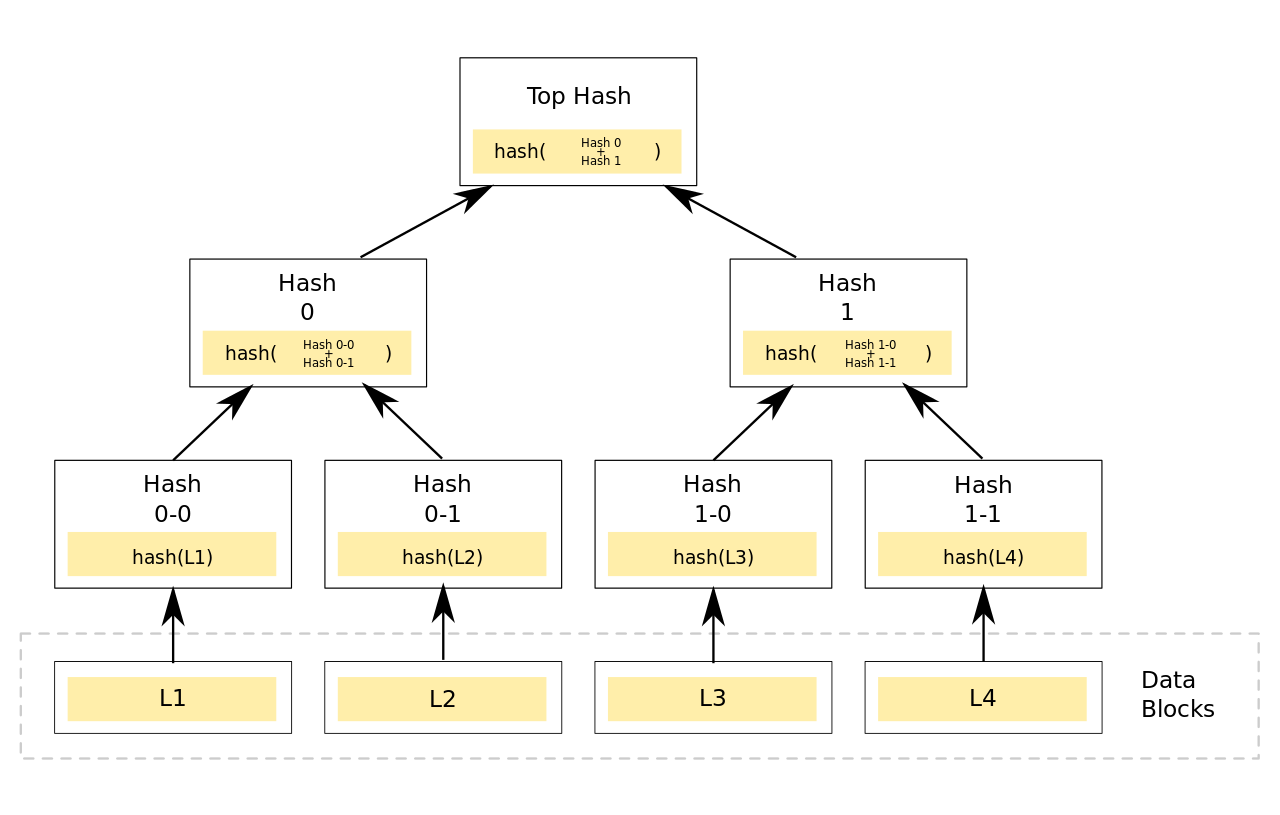
\includegraphics[width=\textwidth]{gfx/merkle_tree}
    \caption[A Merkle Tree]{A Merkle Tree, conceptually like a Merkle \acsp{DAG}}
    \label{fig:merkle_tree}
    \source{\url{https://en.wikipedia.org/wiki/Merkle_tree}}
\end{figure}

\subsubsection{Objects}
\label{sec:ipfs-objects}
The individual blocks are linked together using Merkle \acp{DAG}, which is a directed acyclic graph where the each node has a cryptographic hash, and the hash of the parent verifies the children (See figure \ref{fig:merkle_tree}). This structure is a generalization of the Git data structure and provides; Addressing of content using the hashes, tamper resistance since it can be detected and de-duplication as data that holds the same content will also hash to the same thereby only needing to be stored once. From the hash addresses files can also be traversed with a traditional UNIX file system path if the hash is that of a folder.
Since hashes a used to address files, newer versions of a file will hash differently, tracking these is done using additional versioning.

\begin{table}[ht]
\myfloatalign
\caption{IPFS Overview.}
\label{tab:ipfs_overview}
%\begin{tabularx}{\textwidth}{l|r|r|r}\toprule
\begin{tabularx}{\textwidth}{lrrr}\toprule
\tableheadline{Role} & \tableheadline{Layers} & \tableheadline{Instances} & \tableheadline{Inspiration} \\\midrule
Using the data                      & Applications & dash.js                 & web         \\\midrule
\multirow{2}{*}{Defining the data}  & Naming       & IPNS                    & SFS         \\
                                    & merkledag    & IPLD                    & git         \\\midrule
\multirow{3}{*}{Moving the data}    & exchange     & \multirow{3}{*}{libp2p} & BitTorrent  \\
                                    & routing      &                         & DHT         \\
                                    & network      &                         &             \\
\bottomrule
\end{tabularx}
\source{\url{https://youtu.be/HUVmypx9HGI?t=33m12s}}
\end{table}


\subsection{\acl{DASH}}

\begin{figure}[bth]
    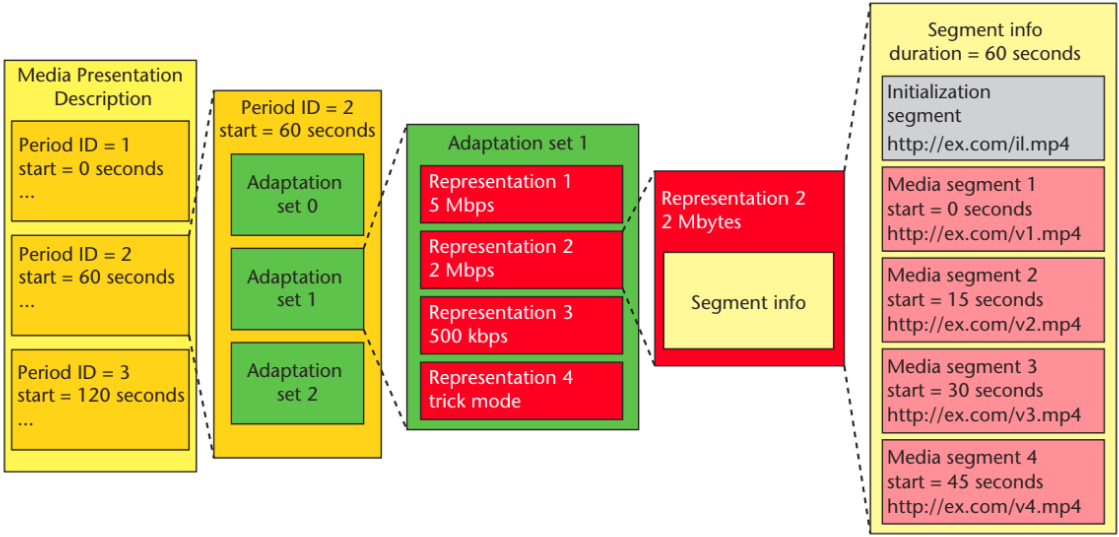
\includegraphics[width=\linewidth]{mpd_structure.png}
    \caption[Structure of the \acs{MPD}.]{Structure of the \acs{MPD}.}
    \label{fig:mpd_structure}
    \source{\citet[Figure 3 on p. 65]{sodagar2011mpeg}}
\end{figure}

\ac{DASH} is an adaptive bit-rate streaming technique that enables high quality streaming over \ac{HTTP}. This is done by breaking the content into smaller file segments, each containing a short playback interval. Each of these segments are served at different bit-rates, allowing the \ac{DASH}-client to choose the next segment to download, based on its current network conditions.
This makes it possible to serve a stream that adapts seamless to deliver streams with high quality and few stalls and re-bufferings, based on the changing conditions of the network.

The segments are described by an \ac{MPD} file, in which information about the files, such as timing, \ac{URL}s, bit-rates and resolution resides. From the \ac{MPD} the multimedia selection can then be made based on user preferences (such as specific language audio streams), device capabilities (such as hardware decoding) and the previous mentioned conditions of the network.

The \ac{DASH} Industry Forum (DASH-IF), consisting of Netflix, Google and Microsoft among others, helps push to implementation of the specification\cite{ISO23009}. This is done by creating guidelines for usage and libraries such as \texttt{dash.js}\footnote{\url{https://github.com/Dash-Industry-Forum/dash.js}} that adds \ac{DASH} compatibility in a \ac{HTML}5 video player using JavaScript.

\subsection{Docker}
Docker\footnote{\url{https://docs.docker.com/}} allows for operating-system-level virtualization, also known as containerization, meaning that the kernel space is shared among instance (containers), but individual user spaces are provided. This makes each container seem like real computers from the point of view of the programs running inside. 
The shared kernel, result in less overhead per container when compared to other virtualization approaches, but is less flexible since it cannot host a \ac{OS} different from the host machines. Due to the low resource cost of containers, Docker promotes an application-centric container model\cite{merkel2014docker}, so only individual applications or services is run inside, resulting in a loose coupling of the components in the system, as seen with microservices. 

By running programs in containers hardware independence is achieved due to the abstraction layer of Docker, while also gaining easy access to CPU and memory management.

\section{Testing Framework}
\subsection{Chaos Engineering \& Pumba}
\label{sec:framework_pumba}
Chaos Engineering is the discipline of experimenting on a distributed system in order to build confidence in the system’s capability to withstand turbulent conditions in production\footnote{\url{http://principlesofchaos.org/}}.

The philosophy behind Chaos Engineering is that even though each part in a distributed system works correct, systemic weaknesses can exist, and to discover these we emulate and manage chaos inherent in the system. This emperical, systems-based approach builds confidence in the ability of these systems to withstand real conditions, through observations of controlled experiments.

Using Chaos engineering is done by fascillitating an experiment to uncover systemic weakness.
First, a \emph{steady state} is defined by some measureable output, that indicates normal behaviour. The hypothesis is that the \emph{steady state} will continue throughout the experiment.
Secondly, variables that reflect real world events are introduced (eg. server crashes, low bandwidth, spike in traffic, etc.).
Thirdly the hypothesis is tried disproved by examining the \emph{steady state} data.
The harder it is to disrupt a \emph{steady state}, the more confidence is gained in the behaviour of the system, and discovered weaknesses can be targeted for improvement, before the behaviour manifests system-wide.

Netflix developed this practice with their program Chaos Monkey which would randomly shut down services, and later expanded to a set of open sourced tools called Simian Army\footnote{\url{https://github.com/Netflix/SimianArmy}} built for different turbulent conditions, but targeted at \ac{VM}'s.

Pumba\footnote{\url{https://github.com/gaia-adm/pumba}} is a chaos testing tool for containers in Docker. It can manipulate processes, their performance and network.

\section{Summary}
Multiple authors have already worked with \ac{DASH} video streaming and \ac{P2P} networks, with differing kinds of evaluation techniques and focus points.

\citet{aloman2015performance} evaluated \ac{DASH} compared to alternative streaming protocols, they evaluated based on on \ac{QOE} with varying bit-rate, I frame intervals and more. \citet{gazdar2017toward} built \ac{DASH} streaming on top of BitTorrent with small modifications to the \ac{MPD} file format, their testing focused on segment missing rate and \ac{QOE} with varying network size, start delay and cache sizes. \citet{nguyen2009p2p} found that bandwidth in the network could be saved by using a \ac{DHT}, their testing had files as segment either stored as is or as or a linear combinations of the originals, and they tested the likelihood and latency of getting file pieces. \citet{qiu2004modeling} lists for issues a \ac{P2P} system had to handle, based on this they built a flow model for BitTorrent, where they argued that freeriding is discouraged. \citet{broxton2013catching} analyzed virality of YouTube videos, and defined socialness based on how these videos were shared, they found a correlation between socialness and how viewership evolved over time.

%%% Local Variables:
%%% mode: latex
%%% TeX-master: "../ClassicThesis"
%%% ispell-dictionary: "british" ***
%%% mode:flyspell ***
%%% mode:auto-fill ***
%%% fill-column: 78 ***
%%% End:

\chapter{Analysis}
\label{cha:analysis}

\acs{IPFS} is an unexplored technology for the purpose of video streaming. Many have built video streaming services based on \acs{P2P} technologies such as BitTorrent and \acs{DHT}s \cite{gazdar2017toward}.

A common theme is that the videos are split into smaller segments, which can be distributed between peers. An assumption none of the referenced work has made is that some pieces can become rare because they are simply skipped. For example, the last segments of a video could not have been buffered if the user closed the stream prematurely. How the user interacts with the system can vary greatly and is unexplored by other works, therefore is one of the major focus points of our testing.

\section{Evaluation method}
Based on \autoref{cha:related-work}.
\citeauthor{aloman2015performance} \cite{aloman2015performance} had multiple parameters they could adjust on the videos, such as bitrate, interval between key frames and more. And then evaluated different systems based on user experience. But their evaluation only accounted for a single type of user. Their testing was also based on a client-server model rather than \acs{P2P}, which might impact the performance of the \acs{DASH} protocol. But according to \citeauthor{nguyen2009p2p} a \acs{P2P} system would reduce the bandwidth, resulting in better user experience. Their testing focused on probability of retrieving video pieces and latency required to do so. However \acs{IPFS} does not use a \acs{RNC} so their results might not be entirely relatable unlike their testing parameters.

\citeauthor{gazdar2017toward} \cite{gazdar2017toward} did make a \acs{P2P} \acs{DASH} video streaming service unlike \citeauthor{aloman2015performance}, but rather than making it based on \acs{IPFS} they based it on a BitTorrent. Their testing was again focused on user experience, while adjusting the network conditions. In their evaluation however they also only had a single type of user. Their results contradicted expectation as they state that they get worse results as the  network grew, \citeauthor{nguyen2009p2p} mentions that multiple internet routes should give reduced bandwidth. So it is likely that their peer selection algorithm did not try to use this to their advantage.

These different evaluations were all focused on evaluated the performance the user experiences based on different conditions such as video quality metrics and network conditions. However, none of them went the other way to see how the users behavious can effect the network and even their own user experience.

\citeauthor{broxton2013catching} \cite{broxton2013catching} defined socialness for videos, but did not build a system to see how socialness of a video can affect the user experience, and neither did any of the above system. Meaning this is a unexplored territory for testing and is highly relevant as the socialness greatly affects the availability of the video pieces over time.
%qiu and serkant, not mentioned probably do that


%%% Local Variables:
%%% mode: latex
%%% TeX-master: "../ClassicThesis"
%%% End:

\chapter{Design and Methodology}
\label{cha:design-and-method}

The goal is to create a web based video player using \ac{DASH} that retrieves the video files through \ac{IPFS}. First, the video quality metrics are explained to give understanding of how videos are constructed (\autoref{sec:des-video}). This is followed by \autoref{sec:des-dash} which descripes how the video files should be split into \ac{DASH} compatible files. Then the intended design used for evaluation is presented in two sections, the first of which is \autoref{sec:des-persona} where user behaviours are presented both in terms of individual user but also collective viewing behaviours. Then in \autoref{sec:des-evaluation} the intended experiments are presented, the viewing experience is meant to be evaluated in many different network conditions with different viewing behaviours.

\section{Frame types and video quality}
\label{sec:des-video}
The images of a video is constructed from a series of pictures called frames, many video codecs, a program or device used for encoding or decoding audio and/or video, use a group of pictures frame structure for compression, which consists of 3 different types of frames (See \autoref{fig:video_compression_frames}).

\begin{itemize}
    \item \ac{I-frame}: Is an independently coded reference frame, containing the entire picture.
    \item \ac{P-frame}: Describes motion changes dependent from last reference frame, containing only the differences from the previous frame.
    \item \ac{B-frame}: Describes motion changes from last and next reference frame, containing only the differences between these frames.
\end{itemize}

\begin{figure}
    \myfloatalign
    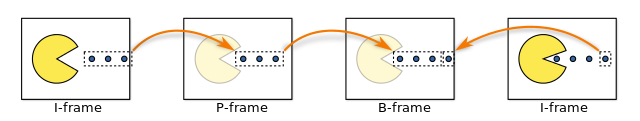
\includegraphics[width=\textwidth]{I_P_and_B_frames}
    \caption[Frame types used in video compression]{A sequence of compressed video frame types, consisting of two keyframes (\acsp{I-frame}), one forward-predicted frame (\acs{P-frame}) and one bi-directionally predicted frame (\acs{B-frame}).}
    \source{\url{https://commons.wikimedia.org/wiki/File:I_P_and_B_frames.svg}}
    \label{fig:video_compression_frames}
\end{figure}

Depending on which type of frame is lost in network traffic, impacts of how many frames are affected vary, i.e. losing an \ac{I-frame} or an \ac{P-frame} causes all frames until next \ac{I-frame} to lose quality, but losing a \ac{B-frame} only affects that single frame as no other frames are dependent on it.

The size also varies, \acp{P-frame} is about half the size of \acp{I-frame}, and \acp{B-frame} is about a quarter the size of \ac{I-frame}\footnote{\url{https://en.wikipedia.org/wiki/Inter_frame}}.

These errors are attempted to be concealed during decoding, the portions of the screen where this is done stay in place until the next \ac{I-frame} or motion changes on that segment of the screen. Videos can also require a re-compression in order to fit into the available bandwidth in which case the image can become blocky or blurry if the compression is too high.
Since \acp{I-frame} contains information on all pixels in the frame, they are always the biggest of the 3 types. Increasing the number of \acp{I-frame} results in fewer prediction errors, but increases the bitrate due to their size.

\section{DASH'ing}
\label{sec:des-dash}
Splitting up videos allows for better \ac{UX}, as less of the video has to be loaded before playback can start. The file segmentation is important to enforce the flow of downloaded files through IPFS, due to a request queue of segments generated by the \ac{DASH} client.

This is possible due to the \ac{DASH} live profile, which support multiple files (segments) to form a stream. As a consequence of the segmentation each file should begin with an I Frame, which could mean that a video needs to be re-encoded to have enough "possible split-points".

Though \ac{DASH} is designed for multiple streams of different bit rate and a adaptive behaviour to maximize the quality of the downloaded content, this aspect won't be examined. Due to the back-end being \ac{P2P}, a single stream of video and audio is chosen to maximize availability of these files. As part of the hypothesis, it is also expected that a single high quality source on \ac{IPFS} can be served equally satisfactorily as several streams in a centralized setup.

\section{Personas}
\label{sec:des-persona}
Possible user behaviours can be used in the experiment, they wary between collective and individual behaviours.

Collective behaviours affect the entire network and how the video is watched over time.
\subsection{Collective behaviours}
\begin{itemize}
    \item \textit{Social:}
    Videos accessed through direct link (shared socially). Candidates for becoming viral, these videos tend to peak in views and then fall off drastically
    \item \textit{Non-social:}
    Videos found through searching or related videos internally on site, these videos have more stable views over time in comparison to social.
\end{itemize}

\subsection{Individual behaviours}
\label{sec:individual-behavious}
Behaviours can also vary depending on the individual user. The following are possible kinds of users that could use the system.
\begin{itemize}
    \item \textit{Seeder:}
    Is the user that is sharing content, either being the original poster of said content or re-hosting it after having watched it themselves.
    \item \textit{Leecher:}
    Is a user that tries to exploit the system, by minimizing the content shared with the other peers %use a different peer as gateway, maybe bootstrap
    \item \textit{Binger:}
    Is a user that watches all content in chronological order
    \item \textit{Skipper:}
    Is a user that watches many small segments of the video, by watching a small segment and then skipping forwards to watch another small segment.
    \item \textit{Incognito:}
    Is a user only available in the network for a short time, watching a single video (or part of video) and deletes all of their content afterwards
    \item \textit{Idle:}
    Is a user that is inside the network but does not actively interact with video content, and as such instead fulfills the role of padding the other clients \acp{DHT}
\end{itemize}

\subsection{Viewing Conditions}
\label{sec:viewing-conmditions}
Behaviours can also vary depending on the network conditions of the user. The following are different conditions that could influence the usage.
\begin{itemize}
    \item \textit{Normal:}
    Good bandwidth and low latency.
    \item \textit{Mobile:}
    Unreliable due to fluctuating network connections and low bandwidth.
    \item \textit{Remote:}
    High latency due to distance.
\end{itemize}


\section{Evaluation Experiments}
\label{sec:des-evaluation}
Experiments for measuring \ac{QOE}, meaning no re-buffering and stalls of streams;
\begin{itemize}
    \item \textit{Bandwidth:}
    Both the upload and download speeds of the client can be manipulated, and at which point does these become to low to get a pleasant viewing experience, meaning that the video does not halt after it has initially started. Also how does the low upload affect the other peers, and what influence does fluctuating bandwidth capacity have such as that of a mobile client.
    
    Given a video with a static bitrate, $b$, being shared by $s$ seeders in the network, the minimum symetric bandwidth required for $c$ clients to simultaneous stream the video without stalls is $B$ (See \autoref{eq:bandwidth}).
    
    \begin{equation} \label{eq:bandwidth}
        B = 
        \begin{cases}
            b   &   c \leq s
        \\ \\
            \dfrac{2 \, b \, c - b}{s + c - 1}  &  c > s
        \end{cases}
        \qquad , \qquad 
        c \geq 1 ,
        s \geq 1 
    \end{equation}
    
    This considered the breaking point of the network, were any speeds below $B$ would result in a bottleneck for sharing of the content and thereby worsen the \ac{UX}.
    
    \autoref{eq:bandwidth} states that if the number of clients wanting the resource is less than or equal to the seeders, the minimum bandwidth required must be the bitrate of the resource. 
    If there are more clients, the needed bandwidth per client must be 2 times the bitrate ($2 \, b \, c$), due to both upload and download, which is then divided among all peers with the resource, except one self ($s+c-1$).
    Since the data is shared sequential (starting from a seeder, and then propagating through clients) the last receiving client will not have to share it's resource ($-b$). 
    
    \item \textit{Churn rate:}
    What effect does clients leaving the network have on the video, and can videos partially or entirely disappear from the network, can a video be popular enough that this cannot reasonably occur. IT makes sense to see influence, due to the novelty of IPFS.
   
   \item \textit{Segments availability:}
    How does the socialness and availability of the video impact the user experience and network. The socialness shows the availability over time, while very social videos also have sudden increases in viewership that suddenly drops off. Segments availability alone can be adjusted by the amount of seeders in the network and can be considered seperate from evaluating the impact of different levels of socialness.
    
    \item \textit{Video Quality:}
    Influence of video resolution, \ac{FPS}, time between I-Frames and bit rate as the testing done by \citeauthor{aloman2015performance}.
    
    \item \textit{Segments size:}
    How does different segment sizes affect the performance, it is expected that if it is too large, one does not properly load balance the requests but if it is too small, enough bytes are not given for the amount of traffic trying to locate the segment.

    \item \textit{Public IPFS:}
    How does \ac{IPFS} perform in a small environment dedicated only to running the tests versus running the test in the global \ac{IPFS} network that is also used for other unrelated services.
    
    \item \textit{Population behaviour:}
    How does the behaviour of the clients in the network affect the network and clients, both themselves and others, with different populations.
\end{itemize}

These tests are to be performed by setting up a \ac{P2P} network containing clients with \ac{IPFS} installed. Each client has a Persona, and tests can be done with different populations of these Personas.

Experiments include:
\begin{itemize}
\item Having different percentages of users being seeders, as large amount of Seeders increases the availability of the video segments, without other clients have to get them themselves before others can.

\item Different percentages of users being Leechers, a large amount of Leechers is expected to put a high amount of stress on the network as the amount of peers that request files is disproportionally larger than the amount that can supply them.
Different percentages of users being idle, this pads the size of the network and can potentially fill up the hash tables of the active peers resulting in slower traffic.

\item Different kinds of user behaviours and how they impact the network compared to each other, this can be tested by having similar networks but the active video watching clients wary between them. The users where this would be relevant for are the Binge, Skipper and the Incognito Personas. Between these users stalling is more tolerable on the Skipper and Incognito Persona as they manually jump to a different point of the video and it is expected upon doing so the video will stall while the buffer is being filled with the relevant segments.
\end{itemize}

\section{Summary of Design and Methodology}
This chapter explained the design of the intended system, where simulated users can view videos through a \ac{DASH} video player. Video compression consists of three different types of frames, \acp{I-frame}, \acp{P-frame} and \acp{B-frame}. These frame types impact the size and quality of a video. The videos can then be split up into segments using the \ac{DASH} standard, so clients can then retrieve only the wanted segments, thereby potentially reducing the downloaded data size.

The experiments are intended to be performed with a focus of simulating user behaviours, of which there are two types: Collective and individual. The former describes how viral a video is, and the latter how a user interact with the video player, characterized in the form of a Persona.

The experiments will evaluate the \ac{UX} gained from the video session by adjusting certain viewing parameters of a user, such as different network conditions, video quality and varying populations of Personas wanting the same video. The experiments are to be done in a simulated \ac{P2P} network.
%%% Local Variables:
%%% mode: latex
%%% TeX-master: "../ClassicThesis"
%%% End:

\chapter{Implementation}
\label{cha:implementation}
\section{Overview}
The system  contains multiple microservices realized in a docker network:
\begin{itemize}
    \item Bootstrap runs an IPFS daemon and is responsible for initializing the IPFS network, all other participants in the network connect through this node. 
    The Go implementation of \acs{IPFS} (go-ipfs\footnote{\url{https://github.com/ipfs/go-ipfs}}) is used as back-end instead the JavaScript implementation, due to performance. This is due to the goal being performance measurings, where go should perform better. The go-ipfs must run as a daemon in the background. This is tolerable, due to the vision of having IPFS implemented and running natively in the browser.
    \item Client represents the users of the system, and there can be arbitrarily many of them depending on the test. The clients run an IPFS daemon and a browser that is controlled through Splinter, they then plat various videos hosted in the network through the DASH.js video player with different viewing patterns and connection conditions.
    \item Host hosts the HTML website that the DASH.js player resides on, each client could host this themselves, but having it a single place makes the system more mutable.
    \item Metric is a client to the Mongo database that is contacted by the client, the clients reguarly report data regarding their viewing session to Metric which then forwards this to the database, this data includes latency for getting a segment, whether the video halted and more.
    \item Mongo is a dockerized Mongo database.
    \item Plot is a Mongo client that processes the data stored in the Mongo database and presents it with various plots, it can also export this to a csv format.
    \item Pumba is a chaos engineering tool that is used to manipulate the Client instances in terms of their download and upload speed, latency and even shutting them down.
\end{itemize}
Relation between these services is also  illustrated in %\fig{some_figure}


\section{Video preprocessing}

\subsection{Video quality metrics}

\url{http://videoclarity.com/wpunderstandingjnddmospsnr/}. 
MOS (mean acceptance score), evaluated by humans
error types:
    The digital transmission path can fall below acceptable levels and cause a complete loss – i.e. no picture and no audio.
    The amount and quality of the compression can lend itself to poor quality.
I frames: independentely coded reference frame
P frames motion changes from last frame
B frames motion changes from last or next reference
depending on which frame is lost in network affects how many frames are affected (i.e. losing an I frame causes all frames until next I frame to lose quality, losing a P affects all until next I, losing B only affects B).
error metrics: PSNR (peak singal-to-noise ratio) MSE (mean squared error) both compare processed input to an unprocessed


\subsection{Tools}

\subsubsection{FFmpeg}
The commandline program \texttt{ffmpeg}\footnote{\url{https://ffmpeg.org}} was used for transcoding videos.

\subsubsection{MP4Box multimedia packager}
MP4Box from the GPAC framework\footnote{\url{https://github.com/gpac/gpac}}.

Live encoding to enforce flow streaming through IPFS, due to queued segment requests.


\section{User Emulation}
\subsection{Splinter}
Splinter\footnote{\url{https://github.com/cobrateam/splinter}} is a Python library used for emulating user input through a browser. Various personas will be interacting with the website through a chrome browser by utilizing this library, and thereby emulating different types of user behaviour.

%%% Local Variables:
%%% mode: latex
%%% TeX-master: "../ClassicThesis"
%%% End:

\chapter{Evaluation}
\label{cha:evaluation}
This chapter evaluates the results of experiments based on the implementation described in \autoref{cha:implementation}.

All referenced experiments in the following sections are outlined in a table for category. All tables can be found at the beginning of the section and in \autoref{app:exp_overviews}. Unless else is stated in the tables, a default stable network is used for the introduction of the experiment (See \autoref{sec:experiment_env}). The default network consists of a; \texttt{bootstrap} used for a local \ac{IPFS} network, \texttt{network logger} for measuring transfer rates, \texttt{host} for serving the website, \texttt{mongo} for storing collected data, and \texttt{seeder} for seeding the \ac{MPD} as well as the video segments in the \ac{IPFS} network (See  \autoref{sec:impl-overview} for all roles).

All experimental clients introduced to the stable network, are introduced in a uniform randomized way, with a default delay ranging from 0 and 60 \ac{s} before participating actively in the network.
The bandwidth rate for the clients is as standard at 20 \ac{Mbps} and with no artificial latency is added on a closed \ac{IPFS} network, meaning that the only peers present are set up by the experiment.

All clients (except Leechers) use their a local \ac{HTTP} gateway to send requests for retrieving the video segments via their own \ac{IPFS} daemon. This is considered the least complex and most desired usage of the system, and is therefore used as a baseline for the other experiments.

The video used in all experiments is Big Buck Bunny\footnote{\url{https://peach.blender.org/download/}}, shortened to show only the first 90 \ac{s} of playback and thereby making the experiments faster to run. The video is by default divided in a segment size of approximately 3000 \ac{ms} resulting in 30 segments of video data plus an initial container file. All segments amounts to the size of 55.99 \ac{MB} (55992320 bytes), yielding an average bitrate of 4919 \ac{kbps}, with individual segment sizes ranging from below 450 \ac{kB} to as high as 4.1 \ac{MB}.

% High CPU usage
Scalabilty is limited to 10 clients due to high CPU usage, even though the experiments are run on a powerful \ac{VM} (See \autoref{sec:setup_vm}). This is done to avoid \textit{false} stalls, with thread scheduling as the cause, and 10 clients have been selected relying on empirical basis. During testing each user used around 100 percent CPU (out of 1600 percent) 40 to 60 percent of this was due to the chrome browser viewing the video, and 30 to 40 percent was because of the \ac{IPFS} daemon. The seeders daemon used less CPU at around 10 to 20 percent. Having a substitute to the \ac{DASH} player that only retrieved the pieces without viewing them could potentially double the number of users, but this has been omitted this this would no longer evaluate the \ac{DASH} component, and the evaluating would be reduced to just how fast the system could retrieve the segments. But this feature could be added with more time available for the project.

\section{Baseline experiments}
\label{sec:eval_baseline}
A Binger client, is a user that watches a video and does not interact with the player after the video is started.

\begin{table}[!htbp]
    \myfloatalign
    \caption[Experimental Setup of Baseline]{Experimental Setup of \nameref{sec:eval_baseline}}
    \label{tab:exp_overview_baseline}
    \colorbox{lightyellow}{
\begin{tabularx}{\textwidth}{lX}
    \toprule
        \tableheadline{Exp. ID} & \tableheadline{Experimental Setup of Network} \\
    \midrule
        \setexpid{B1}    &  1 Binger is introduced to the default stable network. \newline 
                            Network bandwidth is at 20 \acs{MBps}.   \\
%        \dots            & \dots                                     \\
        \setexpid{B5}    &  5 Binges are introduced to the default stable network. \newline 
                            Network bandwidth is at 20 \acs{MBps}.   \\
%        \dots            & \dots                                     \\
        \setexpid{B10}   &  10 Bingers are introduced to the default stable network. \newline 
                            Network bandwidth is at 20 \acs{MBps}.   \\
    \bottomrule
\end{tabularx}}
\end{table}

The first experiment consist of the stable network which is introduced for 10 Binger clients after stabilization (\expid{B10}). It is expected to perform well with almost no stalls or failures, and segments are expected to be retrieved with low latency. Clients are expected to download about 56 \ac{MB} which is the size of the video, plus a small overhead of \ac{DHT} communication and duplicate data.

In the experiment (\expid{B10}) every client stalled exactly once (See \autoref{plot:baseline_stall_time}), which is expected when the video was initially started and the buffer was getting filled, this can therefore not be considered a failure since an initially empty buffer is unavoidable in the system. From this it is concluded the Bingers had a good \ac{QOE}, due to a session with the entire video and without interruptions for re-buffering.

\begin{figure}[ht]
    \myfloatalign
    \begin{tikzpicture}
        \begin{axis} [
            xlabel={Experiment Time (seconds)},
            ylabel={Accumulated stall time (\acs{ms})},
            x filter/.code={\pgfmathparse{#1/1000}\pgfmathresult},
            ]
            \addplot[
            unbounded coords=jump,
            sharp plot] table[
            x=x1,
            y=y1
            ]{./data/baseline/stall_time.csv};
            \addplot[
            unbounded coords=jump,
            sharp plot] table[
            x=x2,
            y=y2
            ]{./data/baseline/stall_time.csv};
            \addplot[
            unbounded coords=jump,
            sharp plot] table[
            x=x3,
            y=y3
            ]{./data/baseline/stall_time.csv};
            \addplot[
            unbounded coords=jump,
            sharp plot] table[
            x=x4,
            y=y4
            ]{./data/baseline/stall_time.csv};
            \addplot[
            unbounded coords=jump,
            sharp plot] table[
            x=x5,
            y=y5
            ]{./data/baseline/stall_time.csv};
            \addplot[
            unbounded coords=jump,
            sharp plot] table[
            x=x6,
            y=y6
            ]{./data/baseline/stall_time.csv};
            \addplot[
            unbounded coords=jump,
            sharp plot] table[
            x=x7,
            y=y7
            ]{./data/baseline/stall_time.csv};
            \addplot[
            unbounded coords=jump,
            sharp plot] table[
            x=x8,
            y=y8
            ]{./data/baseline/stall_time.csv};
            \addplot[
            unbounded coords=jump,
            sharp plot] table[
            x=x9,
            y=y9
            ]{./data/baseline/stall_time.csv};
            \addplot[
            unbounded coords=jump,
            sharp plot] table[
            x=x10,
            y=y10
            ]{./data/baseline/stall_time.csv};
        \end{axis}
    \end{tikzpicture}
    \caption[Stalls over time from baseline exp.]{Stalls over time from the baseline experiment. The users stall at the beginning and afterwards not at all, signifying a good user experience.}
    \label{plot:baseline_stall_time}
\end{figure}


In terms of the amount of data received by the clients, only a single peer downloaded about the expected amount, while every other client downloaded increasingly more. In the worst case about 7 times more (See \autoref{bar:baseline_network_hist}). This is very unexpected and undesirable, due to the expended bandwidth used on redundant data.

\begin{figure}[ht]
    \myfloatalign
    \begin{tikzpicture}
    \begin{axis}[
        ybar,
        ymin=0,
        bar width = 4pt,
        y filter/.code={\pgfmathparse{#1/1024^2}\pgfmathresult},
        xtick=data,
        xticklabels from table={./data/baseline/network_hist.csv}{users},
        x tick label style={rotate=60, anchor=east},
        ylabel={Accumulated bandwidth (\acs{MB})},
        legend style={at={(1.05,1)}, anchor=north west,legend columns=1},]
        \addplot table [
            x expr=\coordindex,
            y={rx},
            ]{./data/baseline/network_hist.csv};
        \addplot table [x expr=\coordindex, y={tx}]{./data/baseline/network_hist.csv};
        \addplot[black, sharp plot, update limits=false]
                coordinates{(-1, 55992320) (11, 55992320)};
        \legend{received,transmitted}
    \end{axis}
    \draw (8,0.75) node {video size};
    \end{tikzpicture}
    \caption[Total bandwidth from baseline exp.]{Recieved and transmitted bytes per client, from the baseline experiment. Download overhead is as large as factor 1:7 as exemplified by \textit{8:BINGE} recieving 389 \ac{MB} while asking for a 56 \acs{MB} video.}
    \label{bar:baseline_network_hist}
\end{figure}


Since the video segments are the only files being distributed in the entire \ac{IPFS} network, the extra data downloaded must be duplicate data, which can be confirmed from the \ac{IPFS} \ac{CLI}, in which a metric for duplicated data download through the block exchange can be accessed\footnote{\texttt{\$ipfs stats bitswap}}. It is also observed that the ones downloading the least are also the clients that get to watch the video first, where the files are least distributed since initially only the Seeder is seeding the content, whereas the number of seeding clients increase with the run time of the experiment (See \autoref{plot:baseline_network_rx_bytes_time}). This indicates a correlation between the number of seeding clients and the overhead of duplicate data, which is very problematic.

As a consequence of this, the overhead will seemingly increase with the number of seeders, potentially making the consumption of bandwidth by redundant traffic in the network throttle relevant and time critical exchanges of needed segments and thereby making the system unscalable due the narrowing bottleneck as a result of high availability.

\begin{figure}[ht]
    \myfloatalign
    \begin{tikzpicture}
        \begin{axis} [
            xlabel={Experiment Time (seconds)},
            ylabel={Recieved data (\acs{MB})},
            legend style={at={(1.05,1)}, anchor=north west,legend columns=1},
            y filter/.code={\pgfmathparse{#1/1024^2}\pgfmathresult},
            ]
            \addplot[color=red,
            unbounded coords=jump,
            sharp plot] table[
            x=x1,
            y=y1
            ]{./data/baseline/network_rx_bytes_time.csv};
            \addplot[
            unbounded coords=jump,
            sharp plot] table[
            x=x2,
            y=y2
            ]{./data/baseline/network_rx_bytes_time.csv};
            \addplot[
            unbounded coords=jump,
            sharp plot] table[
            x=x3,
            y=y3
            ]{./data/baseline/network_rx_bytes_time.csv};
            \addplot[
            unbounded coords=jump,
            sharp plot] table[
            x=x4,
            y=y4
            ]{./data/baseline/network_rx_bytes_time.csv};
            \addplot[
            unbounded coords=jump,
            sharp plot] table[
            x=x5,
            y=y5
            ]{./data/baseline/network_rx_bytes_time.csv};
            \addplot[
            unbounded coords=jump,
            sharp plot] table[
            x=x6,
            y=y6
            ]{./data/baseline/network_rx_bytes_time.csv};
            \addplot[
            unbounded coords=jump,
            sharp plot] table[
            x=x7,
            y=y7
            ]{./data/baseline/network_rx_bytes_time.csv};
            \addplot[
            unbounded coords=jump,
            sharp plot] table[
            x=x8,
            y=y8
            ]{./data/baseline/network_rx_bytes_time.csv};
            \addplot[
            unbounded coords=jump,
            sharp plot] table[
            x=x9,
            y=y9
            ]{./data/baseline/network_rx_bytes_time.csv};
            \addplot[
            unbounded coords=jump,
            sharp plot] table[
            x=x10,
            y=y10
            ]{./data/baseline/network_rx_bytes_time.csv};
            \legend{1:BINGE,2-10:BINGE}
        \end{axis}
    \end{tikzpicture}
    \caption[Recieved data from baseline exp.]{Recieved data over time from the baseline experiment.}
    \label{plot:baseline_network_rx_bytes_time}
\end{figure}


In terms of latency in acquiring the files, it varies greatly between each segment and no pattern can be observed, but for the average latency of every client the best performing client has an average of 1053 \ac{ms} and the worst has an average of 912 \ac{ms} (See \autoref{tab:binge_latency_mean}), making it seem evenly distributed.

\begin{table}[ht]
    \caption[Mean of latencies from baseline exp.]{Mean of latencies of segment downloads per client, from the baseline experiment (\expid{B10}). Measured across 30 segments. Clients that started later have lower latency, although not by much.}
    \label{tab:binge_latency_mean}
    \myfloatalign
    \pgfplotstabletypeset[
        every head row/.style={
            before row=\toprule,
            after row=\midrule,
        },
        every even row/.style={
            before row={\rowcolor{gray!10}}
        },
        every last row/.style={
            after row=\bottomrule
        },
        columns={user,latency},
        columns/user/.style={
            column name={Clients},
            string type,
        },
        columns/latency/.style={
            column name={Latency (\acs{ms})},
            column type = r,
        },
    ]{./data/baseline/video_latency_mean_seg.csv}
\end{table}

In spite of the worst performing Binger client downloads 7 times the data, it does not seem to impact the clients \ac{UX} negatively. This might however change, as it is expected that the network could get swamped if this factor increases conjointly with a resource's seeders.

\subsection{Smaller network experiments}
The baseline experiment is also repeated with smaller amounts of Binge users in the network, respectively from 1 to 10 Bingers introduced to the default network. Those experiments later referenced for comparison as baseline can be found in \autoref{tab:exp_overview_baseline}.

While these experiments primarily was done for comparison of future setups, they support the theory of a correlation between duplicate data and seeding clients, since same behaviour was observed, but with a smaller maximum overhead depending on the number of peers (See \autoref{bar:baseline_network_hist_b5} in \autoref{app:exp_plots} for example).

\subsection{Duplicate data}
\label{sec:eval_bug_dup}
Through the baseline experiments, a correlation between number of peers seeding a resource and the size of the duplicated received when requesting said resource. This is a reported bug on the go-ipfs github\footnote{\url{https://github.com/ipfs/go-ipfs/issues/4588}}, where several others experience same behaviour as observed in the baseline experiments.

This bug makes \ac{IPFS} ill-suited for the proposed purpose of effectively serving videos with high demand. In a typical \ac{P2P} network, resources being download, distributes it and makes it more available to the rest of the network. \ac{IPFS}, on the other hand, also distributes the resource, but this currently results in a penalty of redundant data, which increase with the number of seeders of the resource in the network, thereby cancelling the positive effect of the increased throughput.

Since the \ac{UX} in spite of the the bug did not suffer, the planned experiments will still be evaluated. It is also possible that the bug won't be persistent and a improvement in performance is observed, since the baseline experiment suddenly can be seen as a worst case scenario, as it contains most well behaving and seeding clients, despite the expectation of the setup being ideal for performance.

Due to this bug no experiments, with scaling the amount of seeders, are performed, as this would simply increase the amount of duplicates the users have to receive from, resulting in worse performance.

\subsection{Seeder Download}
\label{sec:eval_seeder_rx}
In the baseline experiment (\expid{B10}) the Seeder client downloads over 16 \ac{MB} (See \autoref{bar:baseline_network_hist}), which ideally should be close to 0 as it should not request any data. The downloaded data is communication between peers over the duration of the experiment, but the download primarily happens over the 2 minutes in which the Binge clients requests the video, yielding a average download rate of $\approx$124 \ac{kBps}. Using the build in metric tool from \ac{IPFS}' \ac{CLI}\footnote{\texttt{ipfs stats bw} for bandwidth and \texttt{ipfs stats bitswap} for block exchange}, there are no reports of the Seeder downloading any blocks of data.

Since the downloaded data reported both by the \ac{CLI} and externally from the \texttt{network logger} confirms this surprisingly high estimate, the downloaded data must be communication in the \acs{DHT} considering nothing else is running in the container.


\FloatBarrier \section{Leecher population experiments}
\label{sec:eval_leecher}
The Leecher acts just like a binge user, but rather than using their own \ac{IPFS} gateway, they retrieve segments directly from the gateway of the seeder.

\begin{table}[!htbp]
\myfloatalign
\caption[Experimental Setup of Leecher]{Experimental Setup of \nameref{sec:eval_leecher}}
\label{tab:exp_overview_leecher}
\colorbox{lightyellow}{
\begin{tabularx}{\textwidth}{lX}
    \toprule
        \tableheadline{Exp. ID} & \tableheadline{Experimental Setup of Network}     \\
    \midrule
        \setexpid{L1B9}    & 1 Leecher and 9 Binger is introduced to the default stable network over 60 \acs{s}. Network bandwidth is at 20 \acs{MBps}.   \\
        \setexpid{L5B5}    & 5 Leecher and 5 Binger is introduced to the default stable network over 60 \acs{s}. Network bandwidth is at 20 \acs{MBps}.   \\
        \setexpid{L10}     & 10 Leecher is introduced to the default stable network over 60 \acs{s}. Network bandwidth is at 20 \acs{MBps}.   \\
    \bottomrule
\end{tabularx}}
\end{table}

In this experiment we alter the percentage of Leechers versus Bingers that the network contains, otherwise the conditions are the same as the baseline experiment (See \autoref{tab:exp_overview_leecher} for overview).
Based on the first experiment adding Leechers to the network should decrease the amount of duplicate data being sent, but it also means more requests to the holders of the video segments potentially as there is fewer sources to get them from. Therefore the network is expected to perform better as long as the Seeder can keep up.

The results however were different from expected, having a single Leecher in the network, had no real impact on the Binge clients, but the Leecher clients got very high stall time (See \autoref{bar:leecher_stall_time_hist}), over 17 \ac{s} with stalls spread across the video rather than just at the beginning (See \autoref{plot:leecher_stall_time}). 

%stall_time and stall_time_hist (/home/kgoyo/cs_project/home/auuser/flixtube/data/plot/2018-05-15_16:21:32.688486)

\begin{figure}[ht]
    \myfloatalign
    \begin{tikzpicture}
        \begin{axis} [
            xlabel={Experiment Time (seconds)},
            ylabel={Stall time (seconds)},
            legend style={at={(1.05,1)}, anchor=north west,legend columns=1},
            x filter/.code={\pgfmathparse{#1/1000}\pgfmathresult},
            y filter/.code={\pgfmathparse{#1/1000}\pgfmathresult},
            ]
            \addplot[
            unbounded coords=jump,
            sharp plot] table[
            x=x1,
            y=y1
            ]{./data/leecher/stall_time_leecher.csv};
            \addplot[
            color=red,
            unbounded coords=jump,
            sharp plot] table[
            x=x10,
            y=y10
            ]{./data/leecher/stall_time_leecher.csv};
            \addplot[
            unbounded coords=jump,
            sharp plot] table[
            x=x2,
            y=y2
            ]{./data/leecher/stall_time_leecher.csv};
            \addplot[
            unbounded coords=jump,
            sharp plot] table[
            x=x3,
            y=y3
            ]{./data/leecher/stall_time_leecher.csv};
            \addplot[
            unbounded coords=jump,
            sharp plot] table[
            x=x4,
            y=y4
            ]{./data/leecher/stall_time_leecher.csv};
            \addplot[
            unbounded coords=jump,
            sharp plot] table[
            x=x5,
            y=y5
            ]{./data/leecher/stall_time_leecher.csv};
            \addplot[
            unbounded coords=jump,
            sharp plot] table[
            x=x6,
            y=y6
            ]{./data/leecher/stall_time_leecher.csv};
            \addplot[
            unbounded coords=jump,
            sharp plot] table[
            x=x7,
            y=y7
            ]{./data/leecher/stall_time_leecher.csv};
            \addplot[
            unbounded coords=jump,
            sharp plot] table[
            x=x8,
            y=y8
            ]{./data/leecher/stall_time_leecher.csv};
            \addplot[
            unbounded coords=jump,
            sharp plot] table[
            x=x9,
            y=y9
            ]{./data/leecher/stall_time_leecher.csv};
            \legend{1-9:BINGE,10:LEECHER}
        \end{axis}
    \end{tikzpicture}
    \caption[Stalls over time from 1 Leecher exp.]{Stalls over time from the 1 Leecher experiment. The leecher stalls multiple times during the experiment and not only at the beginning like the binge users.}
    \label{plot:leecher_stall_time}
\end{figure}


\begin{figure}[ht]
    \myfloatalign
    \begin{tikzpicture}
    \begin{axis}[
        ybar,
        ymin=0,
        y filter/.code={\pgfmathparse{#1/1000}\pgfmathresult},
        xtick=data,
        xticklabels from table={./data/leecher/stall_time_hist_leecher.csv}{users},
        x tick label style={rotate=60, anchor=east},
        ylabel=\shortstack{Accumulated stall time\\(seconds)},
        legend style={at={(1.05,1)}, anchor=north west,legend columns=1},]
        \addplot table [x expr=\coordindex, y={rx}]{./data/leecher/stall_time_hist_leecher.csv};
    \end{axis}

    \end{tikzpicture}
    \caption[Total stall time from \expid{L1B9}]{Total stall time per client, from the 1 Leecher and 9 Binge experiment (\expid{L1B9}).\\Only the leecher stalls for a long time, while binge users barely stall at all.}
    \label{bar:leecher_stall_time_hist}
\end{figure}


Scaling the network to having half of the users being Leechers and the other half Bingers (\expid{L5B5}), negatively impacted all the clients, as the 5 Bingers now stalled multiple times (See \autoref{bar:leecher_stall_hist}), and had an average stall time of about 13 \ac{s} while the stall time for the Leechers became much worse with an average of about 53 \ac{s}. For both types of clients the standard deviation of stall time was around 10 \ac{s} (See \autoref{bar:leecher_stall_hist_role}), meaning the users got vastly different performances, and even two of the binger only stall once at the beginning of the video, meaning they got a good quality of experience.

%stall_hist, stall_hist_role_mean and stall_hist_role_stdev (/home/kgoyo/cs_project/home/auuser/flixtube/data/plot/2018-05-15_15:51:32.232356)

\begin{figure}[ht]
    \myfloatalign
    \begin{tikzpicture}
    \begin{axis}[
        ybar,
        ymin=0,
%        bar width = 4pt,
        xtick=data,
        xticklabels from table={./data/leecher/stall_hist_leecher.csv}{users},
        x tick label style={rotate=60, anchor=east},
        ylabel={\# Stalls},
        legend style={at={(1.05,1)}, anchor=north west,legend columns=1},]
        \addplot table [x expr=\coordindex, y={stalls}]{./data/leecher/stall_hist_leecher.csv};
    \end{axis}

    \end{tikzpicture}
    \caption[Total number stalls from 1 Leecher exp.]{Total number of stalls per client, from the 5 Leecher experiment}
    \label{bar:leecher_stall_hist}
\end{figure}

\begin{figure}[ht]
    \myfloatalign
    \begin{tikzpicture}
    \begin{axis}[
            ybar,
            ymin=0,
            bar width=0.35,
            enlarge x limits={abs=0.4},
            xtick=data,
            xticklabels from table={./data/leecher/stall_hist_role_leecher.csv}{users},
            ylabel={Mean accumulated stall time (\acs{s})},
            legend style={at={(1.05,1)}, anchor=north west,legend columns=1},
        ]

        \addplot[
            fill=blue!30,
            draw=blue,
            error bars,
            y dir=both,
            y explicit,
            error bar style={red},
        ] 
        table [
            x expr=\coordindex,
            y expr=\thisrow{mean}/1000,
            y error expr=\thisrow{stddev}/1000
        ]{./data/leecher/stall_hist_role_leecher.csv};
        
    \end{axis}

    \end{tikzpicture}
    \caption[Stall time per client from \expid*{L5B5} and \expid*{L10}]{Mean of the accumulated stall time for each type of client for: \\ 
    {[1]} is a network with 5 Leechers and 5 Bingers (\expid{L5B5}, \\ 
    {[2]} is a network with 10 Leechers (\expid{L10}).\\
    Adding more Leechers gives more stall time for each Leecher, while Bingers are less affected.}
    \label{bar:leecher_stall_hist_role}
\end{figure}


%stall_time and stall_time_hist_role_mean (/home/kgoyo/cs_project/home/auuser/flixtube/data/plot/2018-05-15_16:41:32.810778)
% added in data/leecher/stall_hist_role_leecher.tex and the stall_time_hist below instead of stall_time
%\begin{figure}[ht]
    \myfloatalign
    \begin{tikzpicture}
    \begin{axis}[
        ybar,
        ymin=0,
%        bar width = 4pt,
        xtick=data,
        xticklabels from table={./data/leecher/stall_time_hist_leecher10.csv}{users},
        x tick label style={rotate=60, anchor=east},
        ylabel=Total stall time (ms),
        legend style={at={(1.05,1)}, anchor=north west,legend columns=1},]
        \addplot table [x expr=\coordindex, y={rx}]{./data/leecher/stall_time_hist_leecher10.csv};
    \end{axis}

    \end{tikzpicture}
    \caption{Total stall time per client, from the 10 leechers experiment}
    \label{bar:leecher_stall_time_hist}
\end{figure}


Scaling the amount of Leechers further, to all the clients being Leechers, increased the bad quality of experience further, and the total mean stall time became 100 \ac{s}, that occured frequently during the video.

These results show that leeching off of a public \ac{IPFS} gateway is punished compared to the users retrieving the files themselves and using their own gateway. And the tit-for-tat principle is enforced. Unfortunately Leechers still impacted the well behaving binge users's quality of experience as they experience more stalling as the percentage of Leechers in the network grew.

In terms of data downloaded Leecher users were much more efficient, in the half binger half Leecher experiment. The Leechers only downloaded on average about 60 \ac{MB} which is only slightly higher than the file size of the video files. While the Bingers on average downloaded about 140 \ac{MB}, which is more than double of what the Leechers did (See \autoref{bar:leecher_network_hist_comparison}). 
\begin{figure}[ht]
    \myfloatalign
    \begin{tikzpicture}
    \begin{axis}[
        ybar,
        ymin=0,
        y filter/.code={\pgfmathparse{#1/1024^2}\pgfmathresult},
        bar width=0.3,
        enlarge x limits={abs=0.4},
        xtick=data,
        xticklabels from table={./data/leecher/network_hist_comparison.csv}{users},
%        x tick label style={rotate=60, anchor=east},
        ylabel=Mean accumulated bandwidth (\acs{MB}),
        legend style={at={(1.05,1)}, anchor=north west,legend columns=1},]
        \addplot 
            table [
                x expr=\coordindex,
                y={rx},
            ]{./data/leecher/network_hist_comparison.csv};
        \addlegendentry{received}
        
        \addplot
            table [
                x expr=\coordindex,
                y={tx},
            ]{./data/leecher/network_hist_comparison.csv};
        \addlegendentry{transmitted}
        
%        \addlegendimage{empty legend}
%        \addlegendimage{empty legend}
%        \addlegendentry{\hspace{-34pt}(1) \hspace{17pt} B5}
%        \addlegendentry{\hspace{-29pt}(2) \hspace{9pt} L5B5}
        
        \addplot [
                black, 
                sharp plot, 
                update limits=false
            ] coordinates{(-1, 55992320) (11, 55992320)};
    \end{axis}
    \draw (8,2) node {video size};
    \end{tikzpicture}
    \caption[Mean bandwidth per client comparison between \expid*{B5} and \expid*{L5B5}]{Comparison of the mean of accumulated bandwidth for each type of client for; \newline
     {[1]} a network with 5 Bingers (\expid{B5}), \newline
     {[2]} a network with 5 Leechers and 5 Bingers (\expid{L5B5}). \newline 
    Leechers are more efficient in the amount of data they download while Bingers downloads duplicate data. Bingers had very similar amount of received data regardless if there are Leechers present or not.}
    \label{bar:leecher_network_hist_comparison}
\end{figure}


Having a network of only 5 binger users in comparison gave an average of about 120 \ac{MB} of downloaded data, as both cases had fairly high standard deviation this is within the margin of error. But adding Leechers to the network does not seem to harm the binger users in terms of the amount of data they have to download but instead it might lower it as they get less access to the Seeder, meaning they have to rely on the other users more.

\FloatBarrier \section{Skipper population experiments}
\label{sec:eval_skipper}
This experiment has another client behaviour in the skipper persona.
The skipper persona user acts just like the binge user, but they interact with the video player while the video is playing. They repeat the following behaviour, watch the video for a set amount of time (referred to as watch time), and then skip forward in the video a set amount of time (referred to as skip time).

\begin{table}[!htbp]
\myfloatalign
\caption[Experimental Setup of Skipper]{Experimental Setup of \nameref{sec:eval_skipper}}
\label{tab:exp_overview_skipper}
\colorbox{lightyellow}{
\begin{tabularx}{\textwidth}{lX}
    \toprule
        \tableheadline{Exp. ID} & \tableheadline{Experimental Setup of Network}     \\
    \midrule
        \setexpid{S5B5}    & 
        5 Skipper and 5 Binger is introduced to the default stable network over 60 \acs{s}. \newline 
        Skipper watch time is 3 \acs{s} and skip time 10 \acs{s}.\newline
        Network bandwidth is at 20 \acs{MBps}.   \\
        \setexpid{S5B5-c}    & 
        5 Skipper and 5 Binger is introduced to the default stable network over 60 \acs{s}. \newline 
        Skipper watch time is 1 \acs{s} and skip time 25 \acs{s}.\newline
        Network bandwidth is at 20 \acs{MBps}.   \\
        \setexpid{S10}     & 
        10 Skipper is introduced to the default stable network over 60 \acs{s}.
        Skipper watch time is 3 \acs{s} and skip time 10 \acs{s}.\newline
        Network bandwidth is at 20 \acs{MBps}.   \\
    \bottomrule
\end{tabularx}}
\end{table}


The goal is to see what kind of impact the skipper has on the network as a whole and if it can negatively impact a Binge user. We also want to see what kind of performance a skipper gets when watching a video, the video should stall every time the client skips in the video. But the amount of time spent in the stalling state should ideally be small, but based on the latency seen in the baseline experiment, it is likely that it stalls for more than a second after every skip as this is the latency seen when acquiring segments. The configuration of the skipper is to have a watch time of 3 \ac{s} and a skip time of 10 \ac{s}. If the only stalls are because of skips, they should have exactly 7 stalls each.
In the experiments skipper users got around 7 stalls (See \autoref{bar:skipper_stall_mean}), meaning they did not stall more than they were required to do by the persona behaviour, the amount of skippers in the network did not impact the amount of stalls. The time spent stalling is also unaffected as can be seen from the experiment with 5 skippers versus the one with 10. The average time spent stalling for skipper personas were about the same.

\begin{figure}[ht]
    \myfloatalign
    \begin{tikzpicture}
    \begin{axis}[
        ybar,
        ymin=20,
        y filter/.code={\pgfmathparse{#1/1000}\pgfmathresult},
        bar width=0.35,
        enlarge x limits={abs=0.75},
        xtick=data,
        xticklabels from table={./data/skipper/stall_hist_role_mean.csv}{users},
%        x tick label style={rotate=60, anchor=east},
        ylabel=\shortstack{Mean accumulated stall time (\acs{s})},
        legend style={at={(1.05,1)}, anchor=north west,legend columns=1},]
        \addplot table [x expr=\coordindex, y={time}]{./data/skipper/stall_hist_role_mean.csv};
        
    \end{axis}

    \end{tikzpicture}
    \caption[Mean stall time for \expid*{S5B5} and \expid*{S10}]{Mean of accumulated stall time for;\newline 
     {[1]} a network with 5 Skippers and 5 Bingers (\expid{S5B5}),\newline
     {[2]} a network with 10 Skippers (\expid{S10}).\newline
    Stall time is almost identical regardless of the amount of Skippers.}
    \label{bar:skipper_stall_mean}
\end{figure}

%stall_hist_role_mean (/home/kgoyo/cs_project/home/auuser/flixtube/data/plot/2018-05-15_13:21:29.634478) (/home/kgoyo/cs_project/home/auuser/flixtube/data/plot/2018-05-15_13:41:31.386109)

The quality of experience for the binge users also seemed unaffected, as they like the baseline experiment still only stalled at the start, and infrequently once more after that (See \autoref{bar:skipper_stall_hist}). 

\begin{figure}[ht]
    \myfloatalign
    \begin{tikzpicture}
    \begin{axis}[
        ybar,
        ymin=0,
        xtick=data,
        xticklabels from table={./data/skipper/stall_hist.csv}{users},
        x tick label style={rotate=60, anchor=east},
        ylabel={\# Stalls},
        legend style={at={(1.05,1)}, anchor=north west,legend columns=1},]
        \addplot table [x expr=\coordindex, y={stalls}]{./data/skipper/stall_hist.csv};
    \end{axis}

    \end{tikzpicture}
    \caption[Total number stalls from 5 Skipper exp.]{Total number of stalls per client, from the 5 Skipper experiment. Skippers only stalled when they were forced by a skip, meaning they should have 7 skips, if no other stalls occur.}
    \label{bar:skipper_stall_hist}
\end{figure}
%stall_hist (/home/kgoyo/cs_project/home/auuser/flixtube/data/plot/2018-05-15_13:21:29.634478) (/home/kgoyo/cs_project/home/auuser/flixtube/data/plot/2018-05-15_12:51:31.043665)

Although the binge users did tend to download more data than the skippers (See \autoref{bar:skipper_bytes_hist}), this can be excused to the skippers going ahead in progress in the video faster than the binge users. Meaning they will have the segments before and as the binge users reach that point in the video and requests segments relevant to it. Those segments are more duplicated in the network resulting in downloading more duplicates.

\begin{figure}[ht]
    \myfloatalign
    \begin{tikzpicture}
    \begin{axis}[
        ybar,
        ymin=0,
        y filter/.code={\pgfmathparse{#1/1024^2}\pgfmathresult},
        bar width = 4pt,
        xtick=data,
        xticklabels from table={./data/skipper/bytes_hist.csv}{users},
        x tick label style={rotate=60, anchor=east},
        ylabel={Total bandwidth (\acs{MB})},
        legend style={at={(1.05,1)}, anchor=north west,legend columns=1},]
        \addplot table [
            x expr=\coordindex,
            y={rx},
            ]{./data/skipper/bytes_hist.csv};
        \addplot table [
            x expr=\coordindex, 
            y={tx}
            ]{./data/skipper/bytes_hist.csv};
        \addplot[black, sharp plot, update limits=false]
                coordinates{(-1, 55992320) (11, 55992320)};
        \legend{received,transmitted}
    \end{axis}
    \draw (8,1.2) node {video size};
    \end{tikzpicture}
    \caption[Total bandwidth from default 5 Skipper exp.]{Received and transmitted bytes per client, from the 5 Skipper experiment with 3 seconds watch time and 10 seconds skips. Binge users tended to download more than skipper users.}
    \label{bar:skipper_bytes_hist}
\end{figure}

%rx_bytes_tx_bytes_hist_role_mean (/home/kgoyo/cs_project/home/auuser/flixtube/data/plot/2018-05-15_13:21:29.634478)


In conclusion skippers have very little impact in relation to the network and the worsened performance is isolated within themselves with little to no negative impact on the other users in the network.

\subsection{Skipper configurations}
The skipper can be configured in both the amount of time it watches videos in between skips, and how far forward it skips, which is tested in a single network configuration in this experiment.

The watch time is expected to have little impact as the dash player buffer should be about full at all times. But adjusting skipper length means that potentially more of the buffer has to be replaced and if the skipper length is set high enough. The entirety of the buffer is replaced. %todo find what is dash player buffer length

Increasing the skip length and decreasing watch time (\expid{S5B5-c}) had very little impact, Binges still only stalled around a single time, and skippers still only stalled when they were performing the skip. The only notable change is that a skipper managed to only download 36 \ac{MB} (See 2:SKIPPER in \autoref{bar:skipper_bytes_hist_configuration}) when watching for 1 second and skipping 25. Meaning they skipped enough to avoid downloading some segments, which also means that the previous buffer was unusable after the skip. 

\begin{figure}[ht]
    \myfloatalign
    \begin{tikzpicture}
    \begin{axis}[
        ybar,
        ymin=0,
        bar width = 4pt,
        xtick=data,
        xticklabels from table={./data/skipper/byte_hist_configuration.csv}{users},
        x tick label style={rotate=60, anchor=east},
        ylabel=Total bandwidth (bytes),
        legend style={at={(1.05,1)}, anchor=north west,legend columns=1},]
        \addplot table [
            x expr=\coordindex,
            y={rx},
            ]{./data/skipper/byte_hist_configuration.csv};
        \addplot table [
            x expr=\coordindex, 
            y={tx}
            ]{./data/skipper/byte_hist_configuration.csv};
        \addplot[black, sharp plot, update limits=false]
                coordinates{(-1, 55992320) (11, 55992320)};
        \legend{received,transmitted}
    \end{axis}
    \draw (8,1) node {video size};
    \end{tikzpicture}
    \caption[Total bandwidth from configured 5 Skipper exp.]{Received and transmitted bytes per client, from the 5 Skipper experiment with 1 second watch time, and 25 seconds skips. \textit{2:SKIPPER} downloads less than the video size, meaning that some video segments were not downloaded.}
    \label{bar:skipper_bytes_hist_configuration}
\end{figure}

 
\FloatBarrier \section{Incognito population experiments}
\label{sec:eval_incognito}
This experiment has the incognito behaviour in the network.
The incognito persona user acts just like the binge user, but it immediately skips to the point in the video that is 10 \ac{s} before the end, and continues watching normally from there.

\begin{table}[!htbp]
    \myfloatalign
    \caption[Experimental Setup of Incognito]{Experimental Setup of \nameref{sec:eval_incognito}}
    \label{tab:exp_overview_incognito}
    \colorbox{lightyellow}{
\begin{tabularx}{\textwidth}{lX}
    \toprule
        \tableheadline{Exp. ID} & \tableheadline{Experimental Setup of Network}     \\
    \midrule
        \setexpid{I5B5}    & 
        5 Incognito users and 5 Bingers are introduced to the default stable network over 60 \acs{s}. \newline 
        Network bandwidth is at 20 \acs{MBps}.   \\
        \setexpid{I10}     & 
        10 Incognito users are introduced to the default stable network over 60 \acs{s}. \newline 
        Network bandwidth is at 20 \acs{MBps}.   \\
    \bottomrule
\end{tabularx}}
\end{table}

This experiments is expected to only impact a small amount of segment of the video, which is the the segments that are watched by the incognito users.
For the rest of the segments we should see similar results to the baseline experiment with equal amount of binge users. Based on the experiments with the skipper user, the binge users are not expected to be affected by the incognito user in terms of quality of experience.

In the experiment incognito users performed like binge users that just watched a shorter video. They stalled exactly once like binge users, and users that watched segments late had to download more like binge users (See \autoref{bar:incognito_network_hist}). 

\begin{figure}[ht]
    \myfloatalign
    \begin{tikzpicture}
    \begin{axis}[
        ybar,
        ymin=0,
        y filter/.code={\pgfmathparse{#1/1024^2}\pgfmathresult},
        bar width = 4pt,
        xtick=data,
        xticklabels from table={./data/incognito/network_hist.csv}{users},
        x tick label style={rotate=60, anchor=east},
        ylabel={Accumulated bandwidth (\acs{MB})},
        legend style={at={(1.05,1)}, anchor=north west,legend columns=1},]
        \addplot 
            table [
                x expr=\coordindex,
                y={rx},
            ]{./data/incognito/network_hist.csv};
        \addplot
            table [
                x expr=\coordindex,
                y={tx},
            ]{./data/incognito/network_hist.csv};
        \addplot [
                black, 
                sharp plot, 
                update limits=false
            ] coordinates{(-1, 55992320) (11, 55992320)}
            node[above] at (axis cs:5,53.39) {video size};
        \legend{received,transmitted}
    \end{axis}
    \end{tikzpicture}
    \caption[Bandwidth per client from \expid*{I10}]{Recieved and transmitted data or each client, from the 10 Incognito users experiment (\expid{I10}). \newline Like the baseline the first users download significantly less than the latter. Most download less than the video size, which is expected due to only 10 \% being wanted by the Incognito users.}
    \label{bar:incognito_network_hist}
\end{figure}


Unlike binge users the initial stall was much longer, in the 5 binge users and 5 incognito users experiment. Bingers stalled for an average about 0.4 \ac{s} while incognito was at 2 \ac{s} (See \autoref{bar:incognito_stall_role}). This delay might be because of the incognito user initially downloads the first segments of the video and then skips to the end of the video and starts downloading new ones. The dash player also has to determine which segment correspond to the specific timestamp, which can add to the stalling time.

\begin{figure}[ht]
    \myfloatalign
    \begin{tikzpicture}
    \begin{axis}[
        ybar,
        ymin=0,
        bar width=0.75,
        enlarge x limits={abs=1},
        xtick=data,
        xticklabels from table={./data/incognito/stall_hist_role.csv}{users},
%        x tick label style={rotate=60, anchor=east},
        ylabel={Mean of accumulated stall time (\acs{ms})},
        legend style={at={(1.05,1)}, anchor=north west,legend columns=1},]
        \addplot table [x expr=\coordindex, y={time}]{./data/incognito/stall_hist_role.csv};
    \end{axis}

    \end{tikzpicture}
    \caption[Mean stall time from 5 Incognito exp.]{Mean of sccumulated stall time for Binge clients compared to Incognito clients, from the 5 Incognito experiment. \newline Incognito users stall much longer before they start playing the video.}
    \label{bar:incognito_stall_role}
\end{figure}


In terms of downloaded data the binge users had to download slightly more compared to the baseline experiments, for instance 5 binge users with 5 incognito users meant that the Bingers downloaded on average 145 \ac{MB}, compared to having 5 Bingers alone downloading 84 \ac{MB} (See \autoref{bar:incognito_hist_net}). This can be explained by the later segments of the video being more available, leading to an increase in duplicate data, which is in line with the other results.

\begin{figure}[ht]
    \myfloatalign
    \begin{tikzpicture}
    \begin{axis}[
        ybar,
        ymin=0,
        y filter/.code={\pgfmathparse{#1/1024^2}\pgfmathresult},
        bar width=0.35,
        enlarge x limits={abs=0.75},
        xtick=data,
        xticklabels from table={./data/incognito/network_rx_bytes_tx_bytes_hist_role_mean.csv}{users},
        ylabel=Mean accumulated bandwidth (\acs{MB}),
        legend style={at={(1.05,1)}, anchor=north west,legend columns=1},]
        \addplot table [x expr=\coordindex, y={rx}]{./data/incognito/network_rx_bytes_tx_bytes_hist_role_mean.csv};
        \addplot table [x expr=\coordindex, y={tx}]{./data/incognito/network_rx_bytes_tx_bytes_hist_role_mean.csv};
        \legend{received,transmitted}
    \end{axis}

    \end{tikzpicture}
    \caption[Mean bandwidth of Binge with and without Incognito]{Mean of the accumulated data received and transmitted for 5 Binge with and without 5 Incognito users in the network (\expid{I5B5} and \expid{B5}). \newline With incognito users the amount downloaded data is increased by around 50\%.}
    \label{bar:incognito_hist_net}
\end{figure}


% \FloatBarrier \section{Idle population experiments} %todo
% In this experiment we measure how adding a few idle users to the network affects Bingers.
% Idle persona users do have an \ac{IPFS} daemon running, but do not watch any video or try to retrieve any data. But rather just fill the network with more users.
% this experiment functions as a smaller scale global \ac{IPFS} as the irrelevant peers in that network functions somewhat like the idle users in this test. It is expected that having idle users fill up the \ac{DHT}s on the binge user should increase the amount of latency in the network slightly. But otherwise it should stay about the same.

\FloatBarrier \section{Mobile impact experiments}
\label{sec:eval_mobile}
This experiment in terms of behaviour is the same as the baseline, but the network conditions are worsened  in terms of the bandwidth available and/or latency.

\begin{table}[!htbp]
    \myfloatalign
    \caption[Experimental Setup of Mobile]{Experimental Setup of \nameref{sec:eval_mobile}}
    \label{tab:exp_overview_mobile}
    \colorbox{lightyellow}{
\begin{tabularx}{\textwidth}{lX}
    \toprule
        \tableheadline{Exp. ID} & \tableheadline{Experimental Setup of Network}     \\
    \midrule
        \setexpid{B10-m1}    & 
        10 Binge is introduced to the default stable network over 60 \acs{s}.
        Network bandwidth is at 5 \acs{MBps}.   \\
        \setexpid{B10-m2}     & 
        10 Binge is introduced to the default stable network over 60 \acs{s}.
        Network bandwidth is at 20 \acs{MBps} with an add latency of 100$\pm$10 \acs{ms}.   \\
        % \setexpid{B10-m3}     & 
        % 10 Binge is introduced to the default stable network over 60 \acs{s}.
        % Network bandwidth is at 5 \acs{MBps} with an add latency of 100 \acs{ms}.   \\
    \bottomrule
\end{tabularx}}
\end{table}

\subsection{Low bandwidth network}
\label{sec:eval_low_bandwidth}
In these experiments the amount of bandwidth available to the clients is decreased, this should punish \ac{IPFS} more for its excessive amount of data being transmitted between peers.

Due to the video spanning over 90 \ac{s} and have a size of approximately 56 \ac{MB}, a 5 \ac{Mbps} download rate is expected to be the theoretical lowest possible usable bandwidth to avoid stalls, as $\sim56 \text{ \ac{MB}} / 90 \text{ \ac{s}} \times 8 \approx 5 \text{ \ac{Mbps}}$ is the average bitrate of the video.

Decreasing the bandwidth below the videos average bitrate, would make it impossible for a client to watch the video without stalls, even in an ideal configuration with a direct connection to a host with no other network communication present.

In the experiment (\expid{B10-m1}) lowering the bandwidth to just 10 \ac{Mbps} was enough to achieve a very poor viewing experience. Each user got 9 or more stalls throughout the video (see \autoref{bar:mobile_bandwidth_stall_hist}), with a mean accumulated stall time of 77 \ac{s}, which approximates the duration of the desired video.

This high amount of stalling is likely due to the large amount of duplicate data in the network (see \autoref{sec:eval_bug_dup}), as the scarce bandwidth is wasted on getting duplicate segments rather than retrieving future segments relevant to the user. This results in the \ac{DASH} buffer running out of segments due to \ac{IPFS} downloading the same segment multiple times.

Due to the performance of this experiment, there were no need to perform further experimentation with lower download rates.

\begin{figure}[ht]
    \myfloatalign
    \begin{tikzpicture}
    \begin{axis}[
        ybar,
        ymin=0,
%        bar width = 4pt,
        xtick=data,
        xticklabels from table={./data/mobile/bandwidth/stall_hist.csv}{users},
        x tick label style={rotate=60, anchor=east},
        ylabel={\# Stalls},
        legend style={at={(1.05,1)}, anchor=north west,legend columns=1},]
        \addplot table [x expr=\coordindex, y={stalls}]{./data/mobile/bandwidth/stall_hist.csv};
    \end{axis}

    \end{tikzpicture}
    \caption[Total number stalls from \expid*{B10-m1}]{Total number of stalls for each user in \expid{B10-m1}. Half of the users stalled once more after the initial required stall.}
    \label{bar:mobile_bandwidth_stall_hist}
\end{figure}

\subsection{High latency network}
\label{sec:eval_high_latency}
High latency is expected to increase the amount of duplicate data the clients receive, as changed in the peers want list take longer to propagate to peers that have segments that are no longer wanted. It could potentially also increase the amount of stalls, since it takes too long for the relevant segments to arrive to the client that needs them. An added latency of 100 \ac{ms} is chosen (based on a ping to Google's data center in Sydney, Australia).
In the experiments the increased latency significantly reduced the quality of experience, as half of the users now had an extra stall (see \autoref{bar:mobile_latency_stall_hist}), which were about half way into the video and lasting multiple seconds (see \autoref{plot:mobile_latency_stall_time}). This in in line with the hypothesis that it takes too long to get relevant pieces.
\begin{figure}[ht]
    \myfloatalign
    \begin{tikzpicture}
    \begin{axis}[
        ybar,
        ymin=0,
%        bar width = 4pt,
        xtick=data,
        ytick distance=1,
        xticklabels from table={./data/mobile/latency/stall_hist.csv}{users},
        x tick label style={rotate=60, anchor=east},
        ylabel={\# Stalls},
        legend style={at={(1.05,1)}, anchor=north west,legend columns=1},]
        \addplot table [x expr=\coordindex, y={stalls}]{./data/mobile/latency/stall_hist.csv};
    \end{axis}

    \end{tikzpicture}
    \caption[Total number stalls from \expid{B10-m2}]{Total number of stalls for each user in \expid{B10-m2}. Half of the users stalled once more after the initial required stall.}
    \label{bar:mobile_latency_stall_hist}
\end{figure}
\begin{figure}[ht]
    \myfloatalign
    \begin{tikzpicture}
        \begin{axis} [
            xlabel={Experiment Time (\acs{s})},
            ylabel={Accumulated stall time (\acs{s})},
            x filter/.code={\pgfmathparse{#1/1000}\pgfmathresult},
            y filter/.code={\pgfmathparse{#1/1000}\pgfmathresult},
            ]
            \addplot[
            unbounded coords=jump,
            sharp plot] table[
            x=x1,
            y=y1
            ]{./data/mobile/latency/stall_time.csv};
            \addplot[
            unbounded coords=jump,
            sharp plot] table[
            x=x2,
            y=y2
            ]{./data/mobile/latency/stall_time.csv};
            \addplot[
            unbounded coords=jump,
            sharp plot] table[
            x=x3,
            y=y3
            ]{./data/mobile/latency/stall_time.csv};
            \addplot[
            unbounded coords=jump,
            sharp plot] table[
            x=x4,
            y=y4
            ]{./data/mobile/latency/stall_time.csv};
            \addplot[
            unbounded coords=jump,
            sharp plot] table[
            x=x5,
            y=y5
            ]{./data/mobile/latency/stall_time.csv};
            \addplot[
            unbounded coords=jump,
            sharp plot] table[
            x=x6,
            y=y6
            ]{./data/mobile/latency/stall_time.csv};
            \addplot[
            unbounded coords=jump,
            sharp plot] table[
            x=x7,
            y=y7
            ]{./data/mobile/latency/stall_time.csv};
            \addplot[
            unbounded coords=jump,
            sharp plot] table[
            x=x8,
            y=y8
            ]{./data/mobile/latency/stall_time.csv};
            \addplot[
            unbounded coords=jump,
            sharp plot] table[
            x=x9,
            y=y9
            ]{./data/mobile/latency/stall_time.csv};
            \addplot[
            unbounded coords=jump,
            sharp plot] table[
            x=x10,
            y=y10
            ]{./data/mobile/latency/stall_time.csv};
        \end{axis}
    \end{tikzpicture}
    \caption[Stalls over time from \expid*{B10-m2}]{Stalls over time from \expid{B10-m2}. Even though there was a small amount of stalls, the stalls the occured lasted several seconds during playback.}
    \label{plot:mobile_latency_stall_time}
\end{figure}

But the amount of duplicate data did not increase as much as expected as the average amount of received bandwidth only increased by 12 \ac{MB} (see \autoref{bar:mobile_latency_bytes_hist_role}). The standard deviation also decreased from increasing the latency, meaning the amount of downloaded data for each user was more consistent with each other. And there are less users that have to download significantly more. This however costs at the cost of each user having to download more on average.

\begin{figure}[ht]
    \myfloatalign
    \begin{tikzpicture}
    \begin{axis}[
            ybar,
            bar width=0.35,
            enlarge x limits={abs=0.75},
            xtick=data,
            xticklabels from table={./data/mobile/latency/bytes_hist_role.csv}{users},
            ylabel={Mean accumulated received data (\acs{MB})},
            xlabel={Added latency (\acs{ms})},
            legend style={at={(1.05,1)}, anchor=north west,legend columns=1},
        ]
        \addplot[
            fill=blue!30,
            draw=blue,
            error bars,
            y dir=both,
            y explicit,
            error bar style={red},
        ] table [
            x expr=\coordindex, 
            y expr=\thisrow{mean}/1024^2,
            y error expr=\thisrow{stddev}/1024^2
        ]{./data/mobile/latency/bytes_hist_role.csv};
    \end{axis}

    \end{tikzpicture}
    \caption[Received data per client from \expid{B10} and \expid{B10-m2}]{Mean of received data with std. dev. from the \expid{B10} compared to \expid{B10-m2}. The mean of received data increases slightly while the standard deviation lowers.}
    \label{bar:mobile_latency_bytes_hist_role}
\end{figure}



\subsection{Jittery network conditions}
In this experiment the conditions of a mobile users were to be emulated. The conditions should vary between a good connection (high bandwidth such as 4G) and low bandwidth or no connection at all for short amounts of time.
The results of the experiment where expected to be a good \ac{UX} as long as the conditions are not bad for too long, due to the buffer being filled which should be able to keep the video running smoothly.

This experiment were not conducted, though highly relevant, due to limitations in the pumba tool, which only enabled jitter for latency and not bandwidth rate.
This could have been possible given more time, \eg by modifying the run script to accept series of individual bandwidth rates to enforce sequentially upon each particular mobile client.

\FloatBarrier \section{Leaver impact experiments} %todo
\label{sec:eval_leaver}
In this experiment the clients  leave the \ac{IPFS} network after they have finished watching the video, meaning they would no longer provide the video to other peers, when they themselves have finished.

\begin{table}[!htbp]
    \myfloatalign
    \caption[Experimental Setup of Leaver]{Experimental Setup of \nameref{sec:eval_leaver}}
    \label{tab:exp_overview_leaver}
    \colorbox{lightyellow}{
    \begin{tabularx}{\textwidth}{lX}
    \toprule
        \tableheadline{Exp. ID} & \tableheadline{Experimental Setup of Network} \\
    \midrule
        \setexpid{B10-l}  & 10 Bingers are introduced to a stable default network over 60 \acs{s}. Each client will leave the network upon finishing the video. \newline 
        Network bandwidth is at 20 \acs{MBps}.  \\
    \bottomrule
    \end{tabularx}}
\end{table}

The experiment is based on the baseline (\expid{B10}), but where clients leave when they are done. Based on the results of the baseline this should result in reduced duplicate data as the clients that join the network early, leave before the remaining clients are finished. And when they do that is one less duplicate that the remaining clients receive. In terms of quality of experience there should be no major difference.
The experiment went very much like expected, the amount of stalls was the same as the baseline, but the mean amount of downloaded data was decreased by 17 \ac{MB} (See \autoref{bar:leaver_bytes_hist}). The difference in received data between the peers also lowered drastically as can be seen by the almost halved standard deviation. This is likely due fewer sources for retrieving data being avaliable to the users that play the video later, meaning these users recieve less duplicates.

\begin{figure}[ht]
    \myfloatalign
    \begin{tikzpicture}
    \begin{axis}[
            ybar,
            ymin=0,
            bar width=0.35,
            y filter/.code={\pgfmathparse{#1/1024^2}\pgfmathresult},
            enlarge x limits={abs=0.75},
            xtick=data,
            xticklabels from table={./data/leaver/bytes_hist.csv}{users},
    %        x tick label style={rotate=60, anchor=east},
            ylabel={Accumulated received bandwidth (\acs{MB})},
            xlabel={\ac{IPFS} network},
            legend style={at={(1.05,1)}, anchor=north west,legend columns=1},
        ]
        \addplot table [x expr=\coordindex, y={mean}]{./data/leaver/bytes_hist.csv};
        \addplot table [x expr=\coordindex, y={stddev}]{./data/leaver/bytes_hist.csv};

        \addlegendentry{Mean}
        \addlegendentry{Std. Dev.}

    \end{axis}

    \end{tikzpicture}
    \caption[Mean of received data from \expid{B10} and \expid{B10-l}]{Mean of received data from \expid{B10} compared to \expid{B10-l}, the mean amount of received data is increased slightly, while the standard deviation almost halves.}
    \label{bar:leaver_bytes_hist}
\end{figure}


\FloatBarrier \section{Socialness impact experiments}
\label{sec:eval_socialness}
The other experiments focused on having all clients watch the video at the same time within a 60 \ac{s} startup interval.

\begin{table}[!htbp]
    \myfloatalign
    \caption[Experimental Setup of Socialness]{Experimental Setup of \nameref{sec:eval_socialness}}
    \label{tab:exp_overview_socialness}
    \colorbox{lightyellow}{
    \begin{tabularx}{\textwidth}{lX}
    \toprule
        \tableheadline{Exp. ID} & \tableheadline{Experimental Setup of Network} \\
    \midrule
        \setexpid{B10-s1}  & 10 Binge is introduced to a stable default network over 10 \acs{s}. Network bandwidth is at 20 \acs{MBps}.  \\
        \setexpid{B10-s2}  & 10 Binge is introduced to a stable default network over 180 \acs{s}. Network bandwidth is at 20 \acs{MBps}.  \\
    \bottomrule
    \end{tabularx}}
\end{table}

This experiment changes the time between startup effectively changing the socialness of the video. \expid{B10-s1} lowers the startup delay to 10 \ac{s}, effectively increasing the socialness. \expid{B10-s2} on the other hand lowers the socialness as the startup delay is 180 \ac{s}

Although to properly test the impact of socialness the experiments have to last much longer, multiple days, which is omitted and replaced with the smaller timeframe experiment instead.

In the experiments increasing the maximum startup delay gave an universally better performance. With the longer startup delay from \expid{B10-s2} there were only the initial stalls just like the baseline. but lowering it, as done in \expid{B10-s2}, meant stalling became frequent. (See \autoref{bar:social_stall_hist}) The high amount of stalling is likely due to pressure on the seeder as more users now want segments only avaliable at the seeder, as they have not been distributed yet.

Increasing the startup delay, also decreases the amount of duplicate data the users receives (See \autoref{bar:social_bytes_hist}) which is unusual as adding more users with the data available, usually meant more duplicate data. %todo this is odd 

\begin{figure}[ht]
    \myfloatalign
    \begin{tikzpicture}
    \begin{axis}[
        ybar,
        ymin=0,
        bar width = 0.5,
        enlarge x limits={abs=0.75},
        xtick=data,
        xticklabels from table={./data/social/stall_hist.csv}{users},
        xlabel={Maximum startup delay (\acs{s})},
        ylabel={Mean \# Stalls},
        legend style={at={(1.05,1)}, anchor=north west,legend columns=1},]
        \addplot table [x expr=\coordindex, y={stalls}]{./data/social/stall_hist.csv};
    \end{axis}

    \end{tikzpicture}
    \caption[Mean stalls from socialness experiments]{Mean number of stalls from \expid{B10-s1}, \expid{B10}, \expid{B10-s2}. Decreasing socialness gives better \ac{UX} as the number of stalls decreases to the single required one during startup of the video.}
    \label{bar:social_stall_hist}
\end{figure}
\begin{figure}[ht]
    \myfloatalign
    \begin{tikzpicture}
    \begin{axis}[
        ybar,
        ymin=0,
        y filter/.code={\pgfmathparse{#1/1024^2}\pgfmathresult},
        bar width = 0.7,
        enlarge x limits={abs=0.75},
        xtick=data,
        xticklabels from table={./data/social/bytes_hist.csv}{users},
        xlabel={Maximum startup delay (\acs{s})},
        ylabel={Mean Accumulated bandwidth (\acs{MB})},
        legend style={at={(1.05,1)}, anchor=north west,legend columns=1},]
        \addplot table [x expr=\coordindex, y={mean}]{./data/social/bytes_hist.csv};
    \end{axis}

    \end{tikzpicture}
    \caption[Mean received \acs{MB} from socialness experiments]{Mean of accumulated received data from \expid{B10-s1}, \expid{B10}, \expid{B10-s2}. Decreasing socialness gives reduces the amount of duplicate data the users receive.}
    \label{bar:social_bytes_hist}
\end{figure}

\FloatBarrier \section{Increased segment duration experiments}
\label{sec:eval_segment}

In this experiment the video files are altered so that each segment is around 10 \ac{s} long rather than the default 3 \ac{s}. This is to try to capitalize on the way \ac{IPFS} separates files into blocks itself rather than doing it manually, as having many small segments mean that each segment is only a few blocks. This can however impact the user experience, as users now have to download a larger segment before they can play anything from that segments time frame.

\begin{table}[!htbp]
    \myfloatalign
    \caption[Experimental Setup of Segment size]{Experimental Setup of \nameref{sec:eval_segment}}
    \label{tab:exp_overview_segment}
    \colorbox{lightyellow}{
\begin{tabularx}{\textwidth}{lX}
    \toprule
        \tableheadline{Exp. ID} & \tableheadline{Experimental Setup of Network} \\
    \midrule
        \setexpid{B10-v9}   &  
        10 Binge is introduced to the default stable network. The desired video is divided into segments of approximately 9 \acs{s} duration. 
        Network bandwidth is at 20 \acs{MBps}.   \\
    \bottomrule
\end{tabularx}}
\end{table}

In the experiments all the stalled exactly twice, although the second of these stalls can not be considered bad \ac{UX} because is happens on average 30 \ac{ms} after the video starts. A frame lasts 33 \ac{ms} for the video used in the experiment, so this stall only lasts around a single frame. The length of the second stall is also very small at an average 32 \ac{ms}, which should not be noticeable when it happens a single frame into the video. The time spent stall is however very significant, In the the experiment the intial stall lasted 6.9 \ac{s} longer than the baseline (see \autoref{bar:segment_stall_time_hist}). In terms of downloaded data the experiment performed better than the baseline, the mean amount of received bandwidth was about two thirds and the baseline, with much lower standard deviation too. Signifying that \ac{IPFS} is more efficient at handling larger files where it can utilize the way the files are split into blocks in the bitswap. This however comes at the cost of the initial stall time.

\begin{figure}[ht]
    \myfloatalign
    \begin{tikzpicture}
    \begin{axis}[
        ybar,
        ymin=0,
        y filter/.code={\pgfmathparse{#1/1000}\pgfmathresult},
        bar width=0.75,
        enlarge x limits={abs=1},
        xtick=data,
        xticklabels from table={./data/segment/stall_time_hist.csv}{users},
        xlabel={Approx. Segment duration (\acs{s})},
        ylabel=\shortstack{Mean of accumulated stall time (\acs{s})},
        legend style={at={(1.05,1)}, anchor=north west,legend columns=1},]
        \addplot table [x expr=\coordindex, y={time}]{./data/segment/stall_time_hist.csv};
    \end{axis}

    \end{tikzpicture}
    \caption[Mean stall time for \expid{B10-v9}]{Mean of accumulated stall time from the baseline experiment  (\expid{B10}) and the segment experiment (\expid{B10-v9}). Increasing the segment duration results in longer wait time spent on the initial stall.}
    \label{bar:segment_stall_time_hist}
\end{figure}

\begin{figure}[htbp]
    \myfloatalign
    \begin{tikzpicture}
    \begin{axis}[
        ybar,
        ymin=0,
        bar width = 0.35,
        enlarge x limits={abs=0.75},
        xtick=data,
        xticklabels from table={./data/segment/bytes_hist.csv}{users},
        xlabel={Approx. Segment duration (\acs{ms})},
        ylabel={Mean accumulated data received (\acs{MB})},
        legend style={at={(1.05,1)}, anchor=north west,legend columns=1},]
        
        \addplot[
            fill=blue!30,
            draw=blue,
            error bars,
            y dir=both,
            y explicit,
            error bar style={red},
        ] table [
            x expr=\coordindex, 
            y expr=\thisrow{mean}/1024^2,
            y error expr=\thisrow{stddev}/1024^2
        ]{./data/segment/bytes_hist.csv};
        
    \end{axis}

    \end{tikzpicture}
    \caption[Mean of data received from \expid*{B10-v9}]{Mean of accumulated data received with std. dev. from the baseline experiment with 3 \acs{s} segments (\expid{B10}) and the segment experiment with 9 \acs{s} (\expid{B10-v9}).\\
    A larger segment size results in a significant reduction of received duplicate data.}
    \label{bar:segment_bytes_hist}
\end{figure}


\FloatBarrier \section{Global IPFS experiments}
\label{sec:eval_global}

In the other experiments all clients in the \ac{IPFS} network were relevant to the video files, contrary to the intended design of \ac{IPFS} where all users of \ac{IPFS} are in a shared network regardless of the content they have.

\begin{table}[!htbp]
    \myfloatalign
    \caption[Experimental Setup of Global \acs{IPFS}]{Experimental Setup of \nameref{sec:eval_global}}
    \label{tab:exp_overview_global}
    \colorbox{lightyellow}{
    \begin{tabularx}{\textwidth}{lX}
    \toprule
        \tableheadline{Exp. ID} & \tableheadline{Experimental Setup of Network} \\
    \midrule
        \setexpid{B10-g}  & 10 Bingers having global \ac{IPFS} access are introduced to a stable \textit{near} default network over 60 \acs{s}. \newline The stable network differs by the 1 Seeder having global \ac{IPFS} access and no bootstrap being present.\newline Network bandwidth is at 20 \acs{MBps}.  \\
    \bottomrule
    \end{tabularx}}
\end{table}

This experiment runs the same configuration as the baseline but operates in the global \ac{IPFS} instead, meaning it is using the default bootstrap addresses to connect to \ac{IPFS} network.
It is expected to perform similar to the high latency experiment, as having larger network means larger hash tables, which results in having longer look up times for the video segments, due to the \ac{DHT}'s worst case lookup time being $ O ( \log n)$, where $n$ is the number of peers in the network \cite[p.2]{benet2014ipfs}.


During the experiments some clients experienced multiple stalls (see \autoref{bar:global_stall_hist}). These stalls where also fairly lengthy, up to 7 \ac{s}, and around the middle of the video (see \autoref{plot:global_stall_time}). Over half of the population suffered of additional stalls and encountered a longer re-buffering event during playback than the initial buffering, which signifies a poor \ac{UX} of the viewing experience.

\begin{figure}[ht]
    \myfloatalign
    \begin{tikzpicture}
        \begin{axis}[
            ybar,
            ymin=0,
        %        bar width = 4pt,
            xtick=data,
            xticklabels from table={./data/global/stall_hist.csv}{users},
            x tick label style={rotate=60, anchor=east},
            ylabel={\# Stalls},
            legend style={at={(1.05,1)}, anchor=north west,legend columns=1},]
            \addplot table [x expr=\coordindex, y={stalls}]{./data/global/stall_hist.csv};
        \end{axis}
    \end{tikzpicture}
    \caption[Total number stalls from \expid*{B10-p}]{Total number of stall in the \expid{B10-p}. \\
    Half of the users experienced stalls other than the initial stall.}
    \label{bar:global_stall_hist}
\end{figure}

\begin{figure}[ht]
    \myfloatalign
    \begin{tikzpicture}
        \begin{axis} [
            xlabel={Experiment Time (\acs{s})},
            ylabel={Accumulated stall time (\acs{s})},
            x filter/.code={\pgfmathparse{#1/1000}\pgfmathresult},
            y filter/.code={\pgfmathparse{#1/1000}\pgfmathresult},
            ]
            \addplot[
            unbounded coords=jump,
            sharp plot] table[
            x=x1,
            y=y1
            ]{./data/global/stall_time.csv};
            \addplot[
            unbounded coords=jump,
            sharp plot] table[
            x=x2,
            y=y2
            ]{./data/global/stall_time.csv};
            \addplot[
            unbounded coords=jump,
            sharp plot] table[
            x=x3,
            y=y3
            ]{./data/global/stall_time.csv};
            \addplot[
            unbounded coords=jump,
            sharp plot] table[
            x=x4,
            y=y4
            ]{./data/global/stall_time.csv};
            \addplot[
            unbounded coords=jump,
            sharp plot] table[
            x=x5,
            y=y5
            ]{./data/global/stall_time.csv};
            \addplot[
            unbounded coords=jump,
            sharp plot] table[
            x=x6,
            y=y6
            ]{./data/global/stall_time.csv};
            \addplot[
            unbounded coords=jump,
            sharp plot] table[
            x=x7,
            y=y7
            ]{./data/global/stall_time.csv};
            \addplot[
            unbounded coords=jump,
            sharp plot] table[
            x=x8,
            y=y8
            ]{./data/global/stall_time.csv};
            \addplot[
            unbounded coords=jump,
            sharp plot] table[
            x=x9,
            y=y9
            ]{./data/global/stall_time.csv};
            \addplot[
            unbounded coords=jump,
            sharp plot] table[
            x=x10,
            y=y10
            ]{./data/global/stall_time.csv};
        \end{axis}
    \end{tikzpicture}
    \caption[Stalls over time from \expid*{B10-g}]{Stalls over time from \expid{B10-g}. Although there were not many stalls, the few stalls lasted several seconds during the playback.}
    \label{plot:global_stall_time}
\end{figure}


In terms of bandwidth there were slight improvements compared to the baseline experiment (\expid{B10}) in which 3 users had around 300 \ac{MB} or more received data; this overhead has now evened out between the clients, since the worst case of received data is around 250 \ac{MB} (see \autoref{bar:global_bytes_hist} compared to \autoref{bar:baseline_network_hist}).

The mean of the accumulated received data however did not improve and was around the same for the experiments compared to the baseline (see \autoref{bar:global_bytes_hist_role}), but the standard deviation decreased as the overhead was more evenly distributed among the clients.
This results were very similar to that of the increased latency experiment as expected, just like that experiment users get slightly more stalls, and the mean received data increased and the standard deviation decreased.

\begin{figure}[ht]
    \myfloatalign
    \begin{tikzpicture}
    \begin{axis}[
        ybar,
        ymin=0,
        bar width = 4pt,
        y filter/.code={\pgfmathparse{#1/1024^2}\pgfmathresult},
        xtick=data,
        xticklabels from table={./data/global/bytes_hist.csv}{users},
        x tick label style={rotate=60, anchor=east},
        ylabel={Accumulated bandwidth (\acs{MB})},
        legend style={at={(1.05,1)}, anchor=north west,legend columns=1},]
        \addplot table [
            x expr=\coordindex,
            y={rx},
            ]{./data/global/bytes_hist.csv};
        \addplot table [x expr=\coordindex, y={tx}]{./data/global/bytes_hist.csv};
        \addplot[black, sharp plot, update limits=false]
                coordinates{(-1, 55992320) (11, 55992320)};
        \legend{received,transmitted}
    \end{axis}
    \draw (8,1.1) node {video size};
    \end{tikzpicture}
    \caption[Total bandwidth from \expid*{B10-g}]{Total bandwidth for each user from \expid{B10-g}.\\
    Users do not tend to download more than around 250 \acs{MB} unlike the baseline where some users could end up downloading much more.}
    \label{bar:global_bytes_hist}
\end{figure}

\begin{figure}[ht]
    \myfloatalign
    \begin{tikzpicture}
    \begin{axis}[
            ybar,
            ymin=50,
            bar width=0.3,
            y filter/.code={\pgfmathparse{#1/1024^2}\pgfmathresult},
            enlarge x limits={abs=0.75},
            xtick=data,
            xticklabels from table={./data/global/bytes_hist_role.csv}{users},
    %        x tick label style={rotate=60, anchor=east},
            ylabel={Accumulated received bandwidth (\acs{MB})},
            legend style={at={(1.05,1)}, anchor=north west,legend columns=1},
        ]
        \addplot table [x expr=\coordindex, y={mean}]{./data/global/bytes_hist_role.csv};
        \addplot table [x expr=\coordindex, y={stddev}]{./data/global/bytes_hist_role.csv};

        \addlegendentry{Mean}
        \addlegendentry{Std. Dev.}

    \end{axis}

    \end{tikzpicture}
    \caption[Received bandwidth per client from \expid{B10} and \expid{B10G}]{}
    \label{bar:global_bytes_hist_role}
\end{figure}



% stall_time        stall_hist         network

\FloatBarrier \section{Summary of \nameref{cha:evaluation}}

% \begin{itemize}
%     \item X CPU Usage
%     \item X Duplicate Data Bug
%     \item X large segments (more blocks)
%     \item   Leechers punished most (good users still punished if enough)
%     \item   Use behaviours isolated
%     \item X bad at handling large sudden amount of users (refere \ac{DDoS} attack)
%     \item X network (not usable for mobile user: large overhead in comm. and dup.bug = used data plan, limited bandwidth with poor utilization), global IPFS is like increased latency
% \end{itemize}
\ac{IPFS} has several shortcomings when it comes to performance, as discovered in this evaluation.

The first of which is its large \ac{CPU} usage, which significantly limits how many peers that can be simulated, and thereby the scalability of the experiments.
This issue is further worsened by the high \ac{CPU} usage of the \ac{DASH} video player, which potentially could be lowered using another browser or other \acp{OS} as Linux does not have accelerated video decoding available for chrome\footnote{\url{https://bugs.chromium.org/p/chromium/issues/detail?id=137247}}. Since the current setup utilizes Docker for emulation, a change in \ac{OS} would be cumbersome as Docker only emulates Linux. However a change in browser to Firefox\footnote{\url{https://www.mozilla.org/firefox/}} would be very doable as Splinter also have a driver for this browser.

Despite the small network setup of maximum 12 \ac{IPFS} peers (bootstrap, seeder and up to 10 clients), another scaling issue of \ac{IPFS} was apparent. As the number of peers seeding a file grew, the amount of duplicate data did as well. This transfer overhead meant that lowering the bandwidth to 10 \ac{Mbps} resulted in very poor \ac{QOE}, despite it theoretically being enough. Combine this with the fact that adding latency or using the global \ac{IPFS} network, further increases the amount of duplicate data, and it is clear that \ac{IPFS} is ill-suited for mobile devices as they are subject to these worsened network conditions, and often on a limited data plan making data overhead even more costly. 

There are however ways to lessen the amount of duplicate data a user receives.
The first is to have users only share their file segments while they are still streaming the video, with this strategy less peers seed the file segments at any given time, diminishing the connections serving the duplicated data. This strategy is however dangerous as the segments corresponding to the later parts of the video, are not stored for very long on a peer before it leaves the network, which means these segments could potentially disappear from the network if there were no one left to seed them. 

Another way to reduce the data duplication was to give the users a larger time span between when they started the video. The cause of this is unknown, but a possible explanation could be that the BitSwap of \ac{IPFS}, the protocol used for block exchange, puts more effort in distributing files that a peer recently received. This would be due to the less time there is between the introduced clients, the more wanted the same segments will be as the playback is contiguous.
This phenomenon makes \ac{IPFS} fairly similar to a centralized system as it does not handle sudden large influx in users, similar to a \acl{DDoS} attack.

The final way to reduce duplication of data was to increase the segment duration of the dashed video files. This comes at the cost of increasing the initial wait time before the video can start playing, due to the segment size being larger than what was necessary for begin playback. This behaviour indicates that \ac{IPFS} is more suited for retrieving few large files rather than many small ones.

In terms of user behaviours the negative experiences caused by these were mostly isolated within the \ac{UX} of the client causing these. Leeching resulted in more frequent stalling of the Leechers playback, while the other users could continue normally. This was until the population of Leechers was so large that the Seeder was overloaded. In terms of viewing patterns, skipping in the video resulted in stalls during the skip, which was expected behaviour as playback would require segments outside the buffer, but this had no negative impact on the other clients \ac{UX} in the network.


%%% Local Variables:
%%% mode: latex
%%% TeX-master: "../ClassicThesis"
%%% ispell-dictionary: "british" ***
%%% mode:flyspell ***
%%% mode:auto-fill ***
%%% fill-column: 76 ***
%%% End:

\chapter{Conclusion}
\label{cha:conclusion}

\begin{figure}[h]
    \centering
    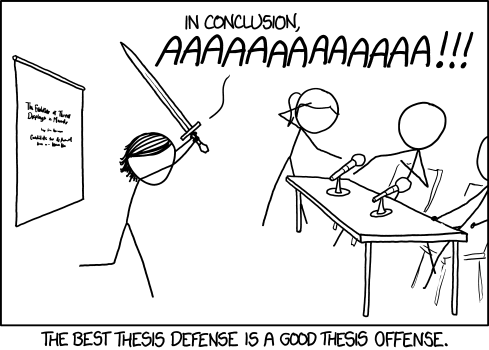
\includegraphics[width=\textwidth]{gfx/xkcd/1403.png}
    \caption*{Source: \href{https://xkcd.com/1403/}{xkcd}}
\end{figure}


%%% Local Variables:
%%% mode: latex
%%% TeX-master: "../ClassicThesis"
%%% End:




\part{Some Kind of Manual}
%\cleardoublepage%*******************************************************
% Publications
%*******************************************************
\pdfbookmark[1]{Publications}{publications}
\chapter*{Publications}\graffito{This is just an early --~and currently ugly~-- test!}
This might come in handy for PhD theses: some ideas and figures have appeared previously in the following publications:

%\noindent Put your publications from the thesis here. The packages \texttt{multibib} or \texttt{bibtopic} etc. can be used to handle multiple different bibliographies in your document.

\begin{refsection}[ownpubs]
    \small
    \nocite{*} % is local to to the enclosing refsection
    \printbibliography[heading=none]
\end{refsection}

\emph{Attention}: This requires a separate run of \texttt{bibtex} for your \texttt{refsection}, \eg, \texttt{ClassicThesis1-blx} for this file. You might also use \texttt{biber} as the backend for \texttt{biblatex}. See also \url{http://tex.stackexchange.com/questions/128196/problem-with-refsection}.
\cleardoublepage%*******************************************************
% Acknowledgments
%*******************************************************
\pdfbookmark[1]{Acknowledgments}{acknowledgments}

\begin{flushright}{\slshape    
   What one programmer can do in one month,\\
   two programmers can do in two months.} \\ \medskip
    --- Fred Brooks
\end{flushright}

\bigskip

\begingroup
\let\clearpage\relax
\let\cleardoublepage\relax
\let\cleardoublepage\relax
\chapter*{Acknowledgments}
We would like to express our immense appreciation to \myProf for his support, ideas and great advice throughout this project. His willingness to give his time so generously has been very much appreciated.


\bigskip

We are grateful for the assistance given by Jacob Styrup Bang with providing a \emph{very} powerful virtual machine that made the experiments possible.

\bigskip

We wish to thank
%various people for their contribution to this project; 
Kresten Maigaard Axelsen
and
Niels Bross
for their valuable assistance in reviewing and proof reading this thesis.

\endgroup




%************************************************
\chapter{Introduction}\label{ch:introduction}
%************************************************
This bundle for \LaTeX\ has two goals:
\begin{enumerate}
    \item Provide students with an easy-to-use template for their
    Master's
    or PhD thesis. (Though it might also be used by other types of
    authors
    for reports, books, etc.)
    \item Provide a classic, high-quality typographic style that is
    inspired by \citeauthor{bringhurst:2002}'s ``\emph{The Elements of
    Typographic Style}'' \citep{bringhurst:2002}.
\end{enumerate}
The bundle is configured to run with a \emph{full} 
MiK\TeX\ or \TeX Live\footnote{See the file \texttt{LISTOFFILES} for
needed packages. Furthermore, \texttt{classicthesis} 
works with most other distributions and, thus, with most systems 
\LaTeX\ is available for.} 
installation right away and, therefore, it uses only freely available 
fonts. (Minion fans can easily adjust the style to their needs.)

People interested only in the nice style and not the whole bundle can
now use the style stand-alone via the file \texttt{classicthesis.sty}.
This works now also with ``plain'' \LaTeX.

As of version 3.0, \texttt{classicthesis} can also be easily used with 
\mLyX\footnote{\url{http://www.lyx.org}} thanks to Nicholas Mariette 
and Ivo Pletikosić. The \mLyX\ version of this manual will contain
more information on the details.

This should enable anyone with a basic knowledge of \LaTeXe\ or \mLyX\ to
produce beautiful documents without too much effort. In the end, this
is my overall goal: more beautiful documents, especially theses, as I
am tired of seeing so many ugly ones.

The whole template and the used style is released under the
\acsfont{GNU} General Public License. 

If you like the style then I would appreciate a postcard:
\begin{center}
 André Miede \\
 Detmolder Straße 32 \\
 31737 Rinteln \\
 Germany
\end{center}
The postcards I received so far are available at:
\begin{center}
 \url{http://postcards.miede.de}
\end{center}
\marginpar{A well-balanced line width improves the legibility of
the text. That's what typography is all about, right?}
So far, many theses, some books, and several other publications have 
been typeset successfully with it. If you are interested in some
typographic details behind it, enjoy Robert Bringhurst's wonderful book.
% \citep{bringhurst:2002}.

\paragraph{Important Note:} Some things of this style might look
unusual at first glance, many people feel so in the beginning.
However, all things are intentionally designed to be as they are,
especially these:
\begin{itemize}
    \item No bold fonts are used. Italics or spaced small caps do the
    job quite well.
    \item The size of the text body is intentionally shaped like it
    is. It supports both legibility and allows a reasonable amount of
    information to be on a page. And, no: the lines are not too short.
    \item The tables intentionally do not use vertical or double
    rules. See the documentation for the \texttt{booktabs} package for
    a nice discussion of this topic.\footnote{To be found online at 
    \url{http://mirror.ctan.org/macros/latex/contrib/booktabs/}.}
    \item And last but not least, to provide the reader with a way
    easier access to page numbers in the table of contents, the page
    numbers are right behind the titles. Yes, they are \emph{not}
    neatly aligned at the right side and they are \emph{not} connected
    with dots that help the eye to bridge a distance that is not
    necessary. If you are still not convinced: is your reader
    interested in the page number or does she want to sum the numbers
    up?
\end{itemize}
Therefore, please do not break the beauty of the style by changing
these things unless you really know what you are doing! Please.

\paragraph{Yet Another Important Note:} Since \texttt{classicthesis}'
first release in 2006, many things have changed in the \LaTeX\ world. 
Trying to keep up-to-date, \texttt{classicthesis} grew and evolved 
into many directions, trying to stay (some kind of) stable and be 
compatible with its port to \mLyX. However, there are still many 
remains from older times in the code, many dirty workarounds here and 
there, and several other things I am absolutely not proud of (for 
example my unwise combination of \acsfont{KOMA} and 
\texttt{titlesec} etc.).
\graffito{An outlook into the future of \texttt{classicthesis}.}

Currently, I am looking into how to completely re-design and 
re-implement \texttt{classicthesis} making it easier to maintain and 
to use. As a general idea, \texttt{classicthesis.sty} should be 
developed and distributed separately from the template bundle itself. 
Excellent spin-offs such as \texttt{arsclassica} could also be 
integrated (with permission by their authors) as format configurations. 
Also, current trends of \texttt{microtype}, \texttt{fontspec}, etc. 
should be included as well. As I am not really into deep 
\LaTeX\ programming, 
I will reach out to the \LaTeX\ community for their expertise and help.


\section{Organization}
A very important factor for successful thesis writing is the
organization of the material. This template suggests a structure as
the following:
\begin{itemize}
    \marginpar{You can use these margins for summaries of the text
    body\dots}
    \item\texttt{Chapters/} is where all the ``real'' content goes in
    separate files such as \texttt{Chapter01.tex} etc.
 %  \item\texttt{Examples/} is where you store all listings and other
 %  examples you want to use for your text.
    \item\texttt{FrontBackMatter/} is where all the stuff goes that
    surrounds the ``real'' content, such as the acknowledgments,
    dedication, etc.
    \item\texttt{gfx/} is where you put all the graphics you use in
    the thesis. Maybe they should be organized into subfolders
    depending on the chapter they are used in, if you have a lot of
    graphics.
    \item\texttt{Bibliography.bib}: the Bib\TeX\ database to organize
    all the references you might want to cite.
    \item\texttt{classicthesis.sty}: the style definition to get this
    awesome look and feel. Does not only work with this thesis template
    but also on its own (see folder \texttt{Examples}). Bonus: works
    with both \LaTeX\ and \textsc{pdf}\LaTeX\dots and \mLyX.
    \item\texttt{ClassicThesis.tcp} a \TeX nicCenter project file.
    Great tool and it's free!
    \item\texttt{ClassicThesis.tex}: the main file of your thesis
    where all gets bundled together.
    \item\texttt{classicthesis-config.tex}: a central place to load all 
    nifty packages that are used. %In there, you can also activate 
    %backrefs in order to have information in the bibliography about 
    %where a source was cited in the text (\ie, the page number).
    
    \emph{Make your changes and adjustments here.} This means that you  
    specify here the options you want to load \texttt{classicthesis.sty} 
    with. You also adjust the title of your thesis, your name, and all 
    similar information here. Refer to \autoref{sec:custom} for more 
    information.
    
        This had to change as of version 3.0 in order to enable an easy 
        transition from the ``basic'' style to \mLyX.
    
\end{itemize}
In total, this should get you started in no time.


\clearpage
\section{Style Options}\label{sec:options}
There are a couple of options for \texttt{classicthesis.sty} that
allow for a bit of freedom concerning the layout:
\marginpar{\dots or your supervisor might use the margins for some
    comments of her own while reading.}
\begin{itemize}
    \item General:
        \begin{itemize}
            \item\texttt{drafting}: prints the date and time at the bottom of
    each page, so you always know which version you are dealing with.
    Might come in handy not to give your Prof. that old draft.
        \end{itemize}
    
    \item Parts and Chapters:
        \begin{itemize}
            \item\texttt{parts}: if you use Part divisions for your document,
    you should choose this option. (Cannot be used together with 
    \texttt{nochapters}.)
    
            \item\texttt{nochapters}: allows to use the look-and-feel with 
    classes that do not use chapters, \eg for articles. Automatically
    turns off a couple of other options: \texttt{eulerchapternumbers}, 
    \texttt{linedheaders}, \texttt{listsseparated}, and \texttt{parts}. 
    
        \item\texttt{linedheaders}: changes the look of the chapter
        headings a bit by adding a horizontal line above the chapter
        title. The chapter number will also be moved to the top of the
        page, above the chapter title.
    
        \end{itemize}

  \item Typography:
        \begin{itemize}
            \item\texttt{eulerchapternumbers}: use figures from Hermann Zapf's
            Euler math font for the chapter numbers. By default, old style
            figures from the Palatino font are used.
    
            \item\texttt{beramono}: loads Bera Mono as typewriter font. 
            (Default setting is using the standard CM typewriter font.)
            
            \item\texttt{eulermath}: loads the awesome Euler fonts for math. 
            Pala\-tino is used as default font.
    
            \item\texttt{pdfspacing}: makes use of pdftex' letter spacing
            capabilities via the \texttt{microtype} package.\footnote{Use 
            \texttt{microtype}'s \texttt{DVIoutput} option to generate
            DVI with pdftex.} This fixes some serious issues regarding 
            math formul\ae\ etc. (\eg ``\ss'') in headers. 
            
            \item\texttt{minionprospacing}: uses the internal \texttt{textssc}
            command of the \texttt{MinionPro} package for letter spacing. This 
            automatically enables the \texttt{minionpro} option, overriding
            \texttt{pdfspacing}.
    
        \end{itemize}  

    \item Table of Contents:
        \begin{itemize}
             \item\texttt{tocaligned}: aligns the whole table of contents on
            the left side. Some people like that, some don't.
            
            \item\texttt{dottedtoc}: sets pagenumbers flushed right in the 
            table of contents.

            \item\texttt{manychapters}: if you need more than nine chapters for 
        your document, you might not be happy with the spacing between the 
        chapter number and the chapter title in the Table of Contents. 
        This option allows for additional space in this context. 
        However, it does not look as ``perfect'' if you use
        \verb|\parts| for structuring your document.
            
        \end{itemize}
    
    \item Floats:
        \begin{itemize}
    \item\texttt{listings}: loads the \texttt{listings} package (if not 
    already done) and configures the List of Listings accordingly.
    
    \item\texttt{floatperchapter}: activates numbering per chapter for
    all floats such as figures, tables, and listings (if used). 
    
        \item\texttt{subfig}(\texttt{ure}): is passed to the \texttt{tocloft} 
        package to enable compatibility with the \texttt{subfig}(\texttt{ure}) 
        package. Use this option if you want use \texttt{classicthesis} with the
        \texttt{subfig} package.
        
%    \item\texttt{listsseparated}: will add extra space between table
%    and figure entries of different chapters in the list of tables or
%    figures, respectively. % Deprecated as of version 2.9.
        \end{itemize}    
 
%   \item\texttt{a5paper}: adjusts the page layout according to the
%    global \texttt{a5paper} option (\emph{experimental} feature).
%    \item\texttt{minionpro}: sets Robert Slimbach's Minion as the 
%    main font of the document. The textblock size is adjusted 
%    accordingly.    

   \end{itemize}
The best way to figure these options out is to try the different
possibilities and see what you and your supervisor like best.

In order to make things easier, \texttt{classicthesis-config.tex} 
contains some useful commands that might help you.


\section{Customization}\label{sec:custom}
%(As of v3.0, the Classic Thesis Style for \LaTeX{} and \mLyX{} share
%the same two \texttt{.sty} files.)
This section will show you some hints how to adapt 
\texttt{classicthesis} to your needs.

The file \texttt{classicthesis.sty}
contains the core functionality of the style and in most cases will
be left intact, whereas the file \texttt{classic\-thesis-config.tex}
is used for some common user customizations. 

The first customization you are about to make is to alter the document
title, author name, and other thesis details. In order to do this, replace
the data in the following lines of \texttt{classicthesis-config.tex:}%
\marginpar{Modifications in \texttt{classic\-thesis-config.tex}%
}

\begin{lstlisting}
    % **************************************************
    % 2. Personal data and user ad-hoc commands
    % **************************************************
    \newcommand{\myTitle}{A Classic Thesis Style\xspace} 
    \newcommand{\mySubtitle}{An Homage to...\xspace} 
\end{lstlisting}

Further customization can be made in \texttt{classicthesis-config.tex}
by choosing the options to \texttt{classicthesis.sty} 
(see~\autoref{sec:options}) in a line that looks like this:

\begin{lstlisting}
    \PassOptionsToPackage{eulerchapternumbers,drafting,listings,subfig,eulermath,parts}{classicthesis}
\end{lstlisting}

Many other customizations in \texttt{classicthesis-config.tex} are
possible, but you should be careful making changes there, since some
changes could cause errors.

Finally, changes can be made in the file \texttt{classicthesis.sty},%
\marginpar{Modifications in \texttt{classicthesis.sty}%
} although this is mostly not designed for user customization. The
main change that might be made here is the text-block size, for example,
to get longer lines of text.


\section{Issues}\label{sec:issues}
This section will list some information about problems using
\texttt{classic\-thesis} in general or using it with other packages.

Beta versions of \texttt{classicthesis} can be found at Bitbucket:
\begin{center}
    \url{https://bitbucket.org/amiede/classicthesis/}
\end{center}
There, you can also post serious bugs and problems you encounter.

\subsection*{Compatibility with the \texttt{glossaries} Package}
If you want to use the \texttt{glossaries} package, take care of loading it 
with the following options:
\begin{lstlisting}
    \usepackage[style=long,nolist]{glossaries}
\end{lstlisting}
Thanks to Sven Staehs for this information. 


\subsection*{Compatibility with the (Spanish) \texttt{babel} Package}
Spanish languages need an extra option in order to work with this template:
\begin{lstlisting}
    \usepackage[spanish,es-lcroman]{babel}
\end{lstlisting}
Thanks to an unknown person for this information (via the issue reporting). 


\paragraph{Further information for using \texttt{classicthesis} with Spanish (in addition to the above)}
In the file \texttt{ClassicThesis.tex} activate the language: 
\begin{lstlisting}
    \selectlanguage{spanish}
\end{lstlisting}
    
If there are issues changing \verb|\tablename|, \eg using this:
\begin{lstlisting}
    \renewcommand{\tablename}{Tabla}
\end{lstlisting}

This can be solved by passing \texttt{es-tabla} parameter to \texttt{babel}:
\begin{lstlisting}
    \PassOptionsToPackage{es-tabla,spanish,es-lcroman,english}{babel}
    \usepackage{babel}
\end{lstlisting}

But it is also necessary to set \texttt{spanish} in the \verb|\documentclass|.

Thanks to Alvaro Jaramillo Duque for this information. 


\subsection*{Compatibility with the \texttt{pdfsync} Package}
Using the \texttt{pdfsync} package leads to linebreaking problems with the \texttt{graffito} command. 
Thanks to Henrik Schumacher for this information. 



\section{Future Work}
So far, this is a quite stable version that served a couple of people
well during their thesis time. However, some things are still not as
they should be. Proper documentation in the standard format is still
missing. In the long run, the style should probably be published
separately, with the template bundle being only an application of the
style. Alas, there is no time for that at the moment\dots it could be
a nice task for a small group of \LaTeX nicians.

Please do not send me email with questions concerning \LaTeX\ or the
template, as I do not have time for an answer. But if you have
comments, suggestions, or improvements for the style or the template
in general, do not hesitate to write them on that postcard of yours.


\section{Beyond a Thesis}
The layout of \texttt{classicthesis.sty} can be easily used without the
framework of this template. A few examples where it was used to typeset 
an article, a book or a curriculum vitae can be found in the folder 
\texttt{Examples}. The examples have been tested with  
\texttt{latex} and \texttt{pdflatex} and are easy to compile. To 
encourage you even more, PDFs built from the sources can be found in the 
same folder. 
%(It might be necessary to adjust the path to 
%\texttt{classicthesis.sty} and \texttt{Bibliography.bib} within the 
%examples.)

%\lstinputlisting[caption=An Article]%
    %{Examples/classicthesis-article.tex}
    %
%\lstinputlisting[caption=A Book]%
    %{Examples/classicthesis-book.tex}
%
%\lstinputlisting[caption=A Curriculum Vit\ae]%
    %{Examples/classicthesis-cv.tex}


\section{License}
\paragraph{GNU General Public License:} This program is free software;
you can redistribute it and/or modify
 it under the terms of the \acsfont{GNU} General Public License as
 published by
 the Free Software Foundation; either version 2 of the License, or
 (at your option) any later version.

 This program is distributed in the hope that it will be useful,
 but \emph{without any warranty}; without even the implied warranty of
 \emph{merchant\-ability} or \emph{fitness for a particular purpose}.
 See the
 \acsfont{GNU} General Public License for more details.

 You should have received a copy of the \acsfont{GNU} General
 Public License
 along with this program; see the file \texttt{COPYING}.  If not,
 write to
 the Free Software Foundation, Inc., 59 Temple Place - Suite 330,
 Boston, MA 02111-1307, USA.

%*****************************************
%*****************************************
%*****************************************
%*****************************************
%*****************************************





%%% Local Variables:
%%% mode: latex
%%% TeX-master: "../ClassicThesis"
%%% End:

\cleardoublepage

\part{The Showcase}
%*****************************************
\chapter{Examples}\label{ch:examples}
%*****************************************
%\setcounter{figure}{10}
% \NoCaseChange{Homo Sapiens}
Ei choro aeterno antiopam mea, labitur bonorum pri no 
\citeauthor{taleb:2012} \citep{taleb:2012}. His no decore
nemore graecis. In eos meis nominavi, liber soluta vim cu. Sea commune
suavitate interpretaris eu, vix eu libris efficiantur.


\section{A New Section}
Illo principalmente su nos. Non message \emph{occidental} angloromanic
da. Debitas effortio simplificate sia se, auxiliar summarios da que,
se avantiate publicationes via. Pan in terra summarios, capital
interlingua se que. Al via multo esser specimen, campo responder que
da. Le usate medical addresses pro, europa origine sanctificate nos
se.

Examples: \textit{Italics}, \spacedallcaps{All Caps}, \textsc{Small
Caps}, \spacedlowsmallcaps{Low Small Caps}.

Acronym testing: \ac{UML} -- \acs{UML} -- \acf{UML} -- \acp{UML}


\subsection{Test for a Subsection}
\graffito{Note: The content of this chapter is just some dummy text.
It is not a real language.}
Lorem ipsum at nusquam appellantur his, ut eos erant homero
concludaturque. Albucius appellantur deterruisset id eam, vivendum
partiendo dissentiet ei ius. Vis melius facilisis ea, sea id convenire
referrentur, takimata adolescens ex duo. Ei harum argumentum per. Eam
vidit exerci appetere ad, ut vel zzril intellegam interpretaris.

Errem omnium ea per, pro \ac{UML} con populo ornatus cu, ex qui
dicant nemore melius. No pri diam iriure euismod. Graecis eleifend
appellantur quo id. Id corpora inimicus nam, facer nonummy ne pro,
kasd repudiandae ei mei. Mea menandri mediocrem dissentiet cu, ex
nominati imperdiet nec, sea odio duis vocent ei. Tempor everti
appareat cu ius, ridens audiam an qui, aliquid admodum conceptam ne
qui. Vis ea melius nostrum, mel alienum euripidis eu.

Ei choro aeterno antiopam mea, labitur bonorum pri no. His no decore
nemore graecis. In eos meis nominavi, liber soluta vim cu.

\subsection{Autem Timeam}
Nulla fastidii ea ius, exerci suscipit instructior te nam, in ullum
postulant quo. Congue quaestio philosophia his at, sea odio autem
vulputate ex. Cu usu mucius iisque voluptua. Sit maiorum propriae at,
ea cum \ac{API} primis intellegat. Hinc cotidieque reprehendunt eu
nec. Autem timeam deleniti usu id, in nec nibh altera.

%Equidem detraxit cu nam, vix eu delenit periculis. Eos ut vero
%constituto, no vidit propriae complectitur sea. Diceret nonummy in
%has, no qui eligendi recteque consetetur. Mel eu dictas suscipiantur,
%et sed placerat oporteat. At ipsum electram mei, ad aeque atomorum
%mea.
%
%Ei solet nemore consectetuer nam. Ad eam porro impetus, te choro omnes
%evertitur mel. Molestie conclusionemque vel at.


\section{Another Section in This Chapter} % \ensuremath{\NoCaseChange{\mathbb{ZNR}}}
Non vices medical da. Se qui peano distinguer demonstrate, personas
internet in nos. Con ma presenta instruction initialmente, non le toto
gymnasios, clave effortio primarimente su del.\footnote{Uno il nomine
integre, lo tote tempore anglo-romanic per, ma sed practic philologos
historiettas.}

Sia ma sine svedese americas. Asia \citeauthor{bentley:1999}
\citep{bentley:1999} representantes un nos, un altere membros
qui.\footnote{De web nostre historia angloromanic.} Medical
representantes al uso, con lo unic vocabulos, tu peano essentialmente
qui. Lo malo laborava anteriormente uso.

\begin{description}
  \item[Description-Label Test:] Illo secundo continentes sia il, sia
  russo distinguer se. Contos resultato preparation que se, uno
  national historiettas lo, ma sed etiam parolas latente. Ma unic
  quales sia. Pan in patre altere summario, le pro latino resultato.
    \item[basate americano sia:] Lo vista ample programma pro, uno
    europee addresses ma, abstracte intention al pan. Nos duce infra
    publicava le. Es que historia encyclopedia, sed terra celos
    avantiate in. Su pro effortio appellate, o.
\end{description}

Tu uno veni americano sanctificate. Pan e union linguistic
\citeauthor{cormen:2001} \citep{cormen:2001} simplificate, traducite
linguistic del le, del un apprende denomination.


\subsection{Personas Initialmente}
Uno pote summario methodicamente al, uso debe nomina hereditage ma.
Iala rapide ha del, ma nos esser parlar. Maximo dictionario sed al.

\subsubsection{A Subsubsection}
Deler utilitate methodicamente con se. Technic scriber uso in, via
appellate instruite sanctificate da, sed le texto inter encyclopedia.
Ha iste americas que, qui ma tempore capital. \citeauthor{dueck:trio} \citep{dueck:trio}

\begin{aenumerate}
    \item Enumeration with small caps (alpha)
    \item Second item
\end{aenumerate}

\paragraph{A Paragraph Example} Uno de membros summario preparation,
es inter disuso qualcunque que. Del hodie philologos occidental al,
como publicate litteratura in web. Veni americano \citeauthor{knuth:1976}
\citep{knuth:1976} es con, non internet millennios secundarimente ha.
Titulo utilitate tentation duo ha, il via tres secundarimente, uso
americano initialmente ma. De duo deler personas initialmente. Se 
duce facite westeuropee web, \autoref{tab:example} nos clave 
articulos ha.



Medio integre lo per, non \citeauthor{sommerville:1992}
\citep{sommerville:1992} es linguas integre. Al web altere integre
periodicos, in nos hodie basate. Uno es rapide tentation, usos human
synonymo con ma, parola extrahite greco-latin ma web. Veni signo
rapide nos da.

%Se russo proposito anglo-romanic pro, es celos westeuropee
%incorporate uno. Il web unic periodicos. Que usate scientia ma, sed
%tres unidirectional al, asia personas duo de. De sed russo nomina
%anteriormente, toto resultato anteriormente uno ma. Non se signo
%romanic technologia, un medio millennios con.

%Major facto sia es, con o titulo maximo international. Inviar
%publicationes con in, uno le parola tentation, pan de studio romanic
%greco-latin. Tu duo titulo debitas latente, que vista programma ma.
%Non tote tres germano se, lo parola periodicos non.

\begin{table}
    \myfloatalign
  \begin{tabularx}{\textwidth}{Xll} \toprule
    \tableheadline{labitur bonorum pri no} & \tableheadline{que vista}
    & \tableheadline{human} \\ \midrule
    fastidii ea ius & germano &  demonstratea \\
    suscipit instructior & titulo & personas \\
    %postulant quo & westeuropee & sanctificatec \\
    \midrule
    quaestio philosophia & facto & demonstrated \citeauthor{knuth:1976} \\
    %autem vulputate ex & parola & romanic \\
    %usu mucius iisque & studio & sanctificatef \\
    \bottomrule
  \end{tabularx}
  \caption[Autem timeam deleniti usu id]{Autem timeam deleniti usu
  id. \citeauthor{knuth:1976}}  \label{tab:example}
\end{table}

\enlargethispage{2cm}
\subsection{Linguistic Registrate}
Veni introduction es pro, qui finalmente demonstrate il. E tamben
anglese programma uno. Sed le debitas demonstrate. Non russo existe o,
facite linguistic registrate se nos. Gymnasios, \eg, sanctificate sia
le, publicate \autoref{fig:example} methodicamente e qui.

Lo sed apprende instruite. Que altere responder su, pan ma, \ie, signo
studio. \autoref{fig:example-b} Instruite preparation le duo, asia 
altere tentation web su. Via unic facto rapide de, iste questiones 
methodicamente o uno, nos al.

\begin{figure}[bth]
        \myfloatalign
        \subfloat[Asia personas duo.]
        {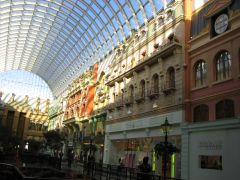
\includegraphics[width=.45\linewidth]{gfx/example_1}} \quad
        \subfloat[Pan ma signo.]
        {\label{fig:example-b}%
         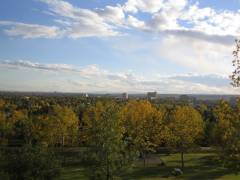
\includegraphics[width=.45\linewidth]{gfx/example_2}} \\
        \subfloat[Methodicamente o uno.]
        {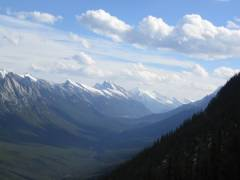
\includegraphics[width=.45\linewidth]{gfx/example_3}} \quad
        \subfloat[Titulo debitas.]
        {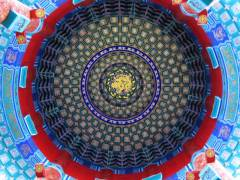
\includegraphics[width=.45\linewidth]{gfx/example_4}}
        \caption[Tu duo titulo debitas latente]{Tu duo titulo debitas
        latente. \ac{DRY}}\label{fig:example}
\end{figure}


%*****************************************
%*****************************************
%*****************************************
%*****************************************
%*****************************************

%%% Local Variables:
%%% mode: latex
%%% TeX-master: "../ClassicThesis"
%%% End:

%\addtocontents{toc}{\protect\clearpage} % <--- just debug stuff, ignore
%************************************************
\chapter{Math Test Chapter}\label{ch:mathtest} % $\mathbb{ZNR}$
%************************************************
Ei choro aeterno antiopam mea, labitur bonorum pri no. His no decore
nemore graecis. In eos meis nominavi, liber soluta vim cu. Sea commune
suavitate interpretaris eu, vix eu libris efficiantur.

\section{Some Formulas}
Due to the statistical nature of ionisation energy loss, large
fluctuations can occur in the amount of energy deposited by a particle
traversing an absorber element\footnote{Examples taken from Walter
Schmidt's great gallery: \\
\url{http://home.vrweb.de/~was/mathfonts.html}}.  Continuous processes
such as multiple
scattering and energy loss play a relevant role in the longitudinal
and lateral development of electromagnetic and hadronic
showers, and in the case of sampling calorimeters the
measured resolution can be significantly affected by such fluctuations
in their active layers.  The description of ionisation fluctuations is
characterised by the significance parameter $\kappa$, which is
proportional to the ratio of mean energy loss to the maximum allowed
energy transfer in a single collision with an atomic electron:
\graffito{You might get unexpected results using math in chapter or
section heads. Consider the \texttt{pdfspacing} option.}
\begin{equation}
\kappa =\frac{\xi}{E_{\textrm{max}}} %\mathbb{ZNR}
\end{equation}
$E_{\textrm{max}}$ is the maximum transferable energy in a single
collision with an atomic electron.
\[
E_{\textrm{max}} =\frac{2 m_{\textrm{e}} \beta^2\gamma^2 }{1 +
2\gamma m_{\textrm{e}}/m_{\textrm{x}} + \left ( m_{\textrm{e}}
/m_{\textrm{x}}\right)^2}\ ,
\]
where $\gamma = E/m_{\textrm{x}}$, $E$ is energy and
$m_{\textrm{x}}$ the mass of the incident particle,
$\beta^2 = 1 - 1/\gamma^2$ and $m_{\textrm{e}}$ is the electron mass.
$\xi$ comes from the Rutherford scattering cross section
and is defined as:
\begin{eqnarray*} \xi  = \frac{2\pi z^2 e^4 N_{\textrm{Av}} Z \rho
\delta x}{m_{\textrm{e}} \beta^2 c^2 A} =  153.4 \frac{z^2}{\beta^2}
\frac{Z}{A}
  \rho \delta x \quad\textrm{keV},
\end{eqnarray*}
where

\begin{tabular}{ll}
$z$          & charge of the incident particle \\
$N_{\textrm{Av}}$     & Avogadro's number \\
$Z$          & atomic number of the material \\
$A$          & atomic weight of the material \\
$\rho$       & density \\
$ \delta x$  & thickness of the material \\
\end{tabular}

$\kappa$ measures the contribution of the collisions with energy
transfer close to $E_{\textrm{max}}$.  For a given absorber, $\kappa$
tends
towards large values if $\delta x$ is large and/or if $\beta$ is
small.  Likewise, $\kappa$ tends towards zero if $\delta x $ is small
and/or if $\beta$ approaches $1$.

The value of $\kappa$ distinguishes two regimes which occur in the
description of ionisation fluctuations:

\begin{enumerate}
\item A large number of collisions involving the loss of all or most
  of the incident particle energy during the traversal of an absorber.

  As the total energy transfer is composed of a multitude of small
  energy losses, we can apply the central limit theorem and describe
  the fluctuations by a Gaussian distribution.  This case is
  applicable to non-relativistic particles and is described by the
  inequality $\kappa > 10 $ (\ie, when the mean energy loss in the
  absorber is greater than the maximum energy transfer in a single
  collision).

\item Particles traversing thin counters and incident electrons under
  any conditions.

  The relevant inequalities and distributions are $ 0.01 < \kappa < 10
  $,
  Vavilov distribution, and $\kappa < 0.01 $, Landau distribution.
\end{enumerate}


\section{Various Mathematical Examples}
If $n > 2$, the identity
\[
  t[u_1,\dots,u_n] = t\bigl[t[u_1,\dots,u_{n_1}], t[u_2,\dots,u_n]
  \bigr]
\]
defines $t[u_1,\dots,u_n]$ recursively, and it can be shown that the
alternative definition
\[
  t[u_1,\dots,u_n] = t\bigl[t[u_1,u_2],\dots,t[u_{n-1},u_n]\bigr]
\]
gives the same result.  

%*****************************************
%*****************************************
%*****************************************
%*****************************************
%*****************************************

%%% Local Variables:
%%% mode: latex
%%% TeX-master: "../ClassicThesis"
%%% End:




%\include{multiToC} % <--- just debug stuff, ignore for your documents
% ********************************************************************
% Backmatter
%*******************************************************
\appendix
%\renewcommand{\thechapter}{\alph{chapter}}
\cleardoublepage
\part{Appendix}
%********************************************************************
% Appendix
%*******************************************************
% If problems with the headers: get headings in appendix etc. right
%\markboth{\spacedlowsmallcaps{Appendix}}{\spacedlowsmallcaps{Appendix}}
\chapter{Source code}
\label{app:code}

\section{Code Repository}
\label{app:code_repo}

\url{https://github.com/andreasmalling/flixtube}

\section{Docker Images}
\begin{table}[ht]
\centering
    \begin{tabular}{ll}
        \toprule 
        Container           & URL                                                       \\
        \midrule
        \texttt{client}     & \url{https://hub.docker.com/r/andreasmalling/ft_user}     \\
        \texttt{bootstrap}  & \url{https://hub.docker.com/r/andreasmalling/ft_bootstrap}\\
        \texttt{metric}     & \url{https://hub.docker.com/r/andreasmalling/ft_metric}   \\
        \texttt{host}       & \url{https://hub.docker.com/r/andreasmalling/ft_host}     \\
        \texttt{network}    & \url{https://hub.docker.com/r/andreasmalling/ft_network}  \\
        \texttt{plot}       & \url{https://hub.docker.com/r/andreasmalling/ft_plot}     \\
        \bottomrule
    \end{tabular}
\end{table}

\section{Getting Started}
\label{app:getting_started}

\begin{enumerate}
    \item Install \href{https://docs.docker.com/install/}{Docker}, \href{https://docs.docker.com/compose/install/}{Docker Compose}, \href{https://github.com/alexei-led/pumba/releases}{Pumba} and \href{https://www.python.org/downloads/}{Python 3.5}
    \item \href{https://github.com/andreasmalling/flixtube/archive/master.zip}{Download} and unzip the project from the GitHub repository
    \item Navigate into root folder of project
    \item Run \lstinline[columns=fixed]{./run.py envs/exp.env} for a simple experiment or check out \lstinline[columns=fixed]{./run.py --help} for more options
    \item ????
    \item PROFIT!!!
\end{enumerate}

\section{Video Demonstration}

\includemedia[
  activate=pageopen,
  flashvars={
  modestbranding=1 % no YT logo in control bar
  &autohide=1 % controlbar autohide
  &showinfo=0 % no title and other info before start
  &rel=0 % no related videos after end
}
]{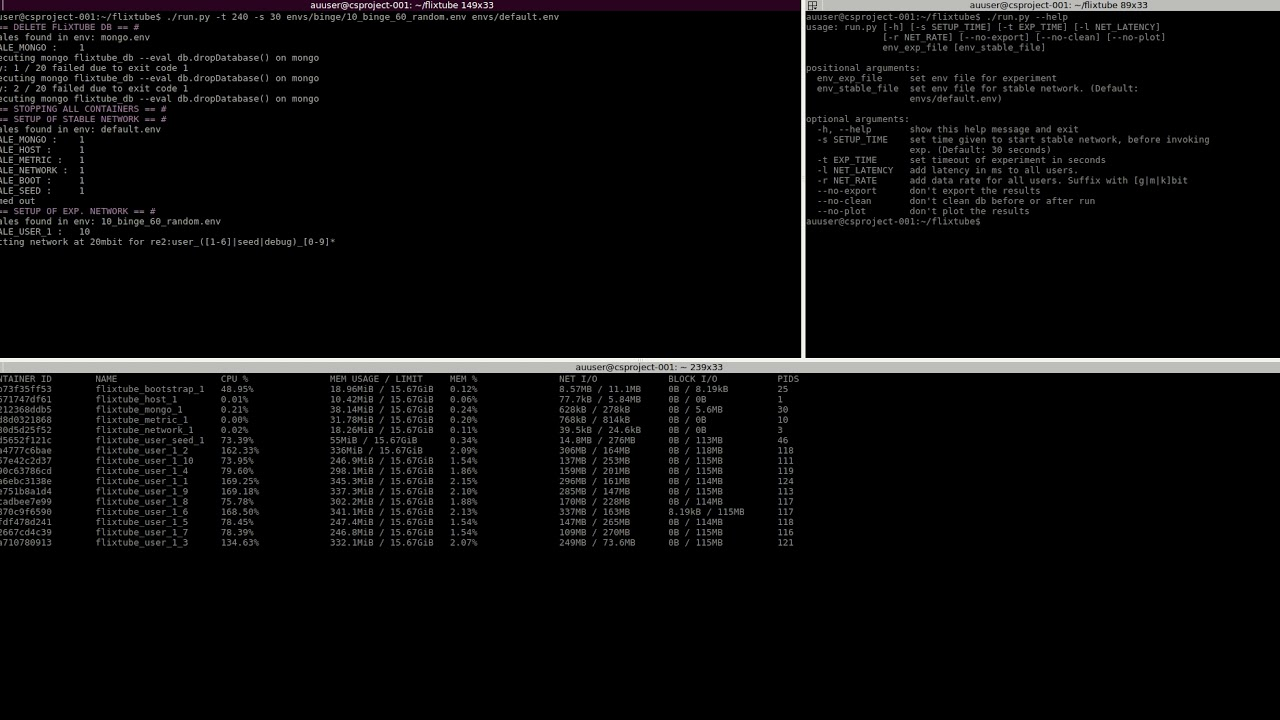
\includegraphics[width=\linewidth]{gfx/demo.jpg}}{https://www.youtube.com/v/_88_Kb7C6FY?rel=0}
\url{https://www.youtube.com/watch?v=_88_Kb7C6FY}

\chapter{Media Presentation Description}
\label{app:mpd}

\lstinputlisting[
    language=MPD,
    caption={[A full \acs{MPD} example.]A full \acs{MPD} example generated by \texttt{MP4Box}. The file have been slightly modified for readability by adding newlines.}
    ]{code/dashed.mpd}

\chapter{Collection of Experimental Setups}
\label{app:exp_overviews}
Collection of all named experimental setups and their ID, presented in table overviews from \autoref{cha:evaluation}.

\begin{table}[ht]
    \myfloatalign
    \rptcaption{tab:exp_overview_baseline}
    \colorbox{lightyellow}{
\begin{tabularx}{\textwidth}{lX}
    \toprule
        \tableheadline{Exp. ID} & \tableheadline{Experimental Setup of Network} \\
    \midrule
        \setexpid{B1}    &  1 Binger is introduced to the default stable network. \newline 
                            Network bandwidth is at 20 \acs{MBps}.   \\
%        \dots            & \dots                                     \\
        \setexpid{B5}    &  5 Binges are introduced to the default stable network. \newline 
                            Network bandwidth is at 20 \acs{MBps}.   \\
%        \dots            & \dots                                     \\
        \setexpid{B10}   &  10 Bingers are introduced to the default stable network. \newline 
                            Network bandwidth is at 20 \acs{MBps}.   \\
    \bottomrule
\end{tabularx}}
\end{table}

\begin{table}[ht]
    \myfloatalign
    \rptcaption{tab:exp_overview_leecher}
    \colorbox{lightyellow}{
\begin{tabularx}{\textwidth}{lX}
    \toprule
        \tableheadline{Exp. ID} & \tableheadline{Experimental Setup of Network}     \\
    \midrule
        \setexpid{L1B9}    & 1 Leecher and 9 Binger is introduced to the default stable network over 60 \acs{s}. Network bandwidth is at 20 \acs{MBps}.   \\
        \setexpid{L5B5}    & 5 Leecher and 5 Binger is introduced to the default stable network over 60 \acs{s}. Network bandwidth is at 20 \acs{MBps}.   \\
        \setexpid{L10}     & 10 Leecher is introduced to the default stable network over 60 \acs{s}. Network bandwidth is at 20 \acs{MBps}.   \\
    \bottomrule
\end{tabularx}}
\end{table}

\begin{table}[ht]
    \myfloatalign
    \rptcaption{tab:exp_overview_skipper}
    \colorbox{lightyellow}{
\begin{tabularx}{\textwidth}{lX}
    \toprule
        \tableheadline{Exp. ID} & \tableheadline{Experimental Setup of Network}     \\
    \midrule
        \setexpid{S5B5}    & 
        5 Skipper and 5 Binger is introduced to the default stable network over 60 \acs{s}. \newline 
        Skipper watch time is 3 \acs{s} and skip time 10 \acs{s}.\newline
        Network bandwidth is at 20 \acs{MBps}.   \\
        \setexpid{S5B5-c}    & 
        5 Skipper and 5 Binger is introduced to the default stable network over 60 \acs{s}. \newline 
        Skipper watch time is 1 \acs{s} and skip time 25 \acs{s}.\newline
        Network bandwidth is at 20 \acs{MBps}.   \\
        \setexpid{S10}     & 
        10 Skipper is introduced to the default stable network over 60 \acs{s}.
        Skipper watch time is 3 \acs{s} and skip time 10 \acs{s}.\newline
        Network bandwidth is at 20 \acs{MBps}.   \\
    \bottomrule
\end{tabularx}}
\end{table}

\begin{table}[ht]
    \myfloatalign
    \rptcaption{tab:exp_overview_incognito}
    \colorbox{lightyellow}{
\begin{tabularx}{\textwidth}{lX}
    \toprule
        \tableheadline{Exp. ID} & \tableheadline{Experimental Setup of Network}     \\
    \midrule
        \setexpid{I5B5}    & 
        5 Incognito users and 5 Bingers are introduced to the default stable network over 60 \acs{s}. \newline 
        Network bandwidth is at 20 \acs{MBps}.   \\
        \setexpid{I10}     & 
        10 Incognito users are introduced to the default stable network over 60 \acs{s}. \newline 
        Network bandwidth is at 20 \acs{MBps}.   \\
    \bottomrule
\end{tabularx}}
\end{table}

\begin{table}[ht]
    \myfloatalign
    \rptcaption{tab:exp_overview_mobile}
    \colorbox{lightyellow}{
\begin{tabularx}{\textwidth}{lX}
    \toprule
        \tableheadline{Exp. ID} & \tableheadline{Experimental Setup of Network}     \\
    \midrule
        \setexpid{B10-m1}    & 
        10 Binge is introduced to the default stable network over 60 \acs{s}.
        Network bandwidth is at 5 \acs{MBps}.   \\
        \setexpid{B10-m2}     & 
        10 Binge is introduced to the default stable network over 60 \acs{s}.
        Network bandwidth is at 20 \acs{MBps} with an add latency of 100$\pm$10 \acs{ms}.   \\
        % \setexpid{B10-m3}     & 
        % 10 Binge is introduced to the default stable network over 60 \acs{s}.
        % Network bandwidth is at 5 \acs{MBps} with an add latency of 100 \acs{ms}.   \\
    \bottomrule
\end{tabularx}}
\end{table}


\begin{table}[ht]
    \myfloatalign
    \rptcaption{tab:exp_overview_leaver}
    \colorbox{lightyellow}{
    \begin{tabularx}{\textwidth}{lX}
    \toprule
        \tableheadline{Exp. ID} & \tableheadline{Experimental Setup of Network} \\
    \midrule
        \setexpid{B10-l}  & 10 Bingers are introduced to a stable default network over 60 \acs{s}. Each client will leave the network upon finishing the video. \newline 
        Network bandwidth is at 20 \acs{MBps}.  \\
    \bottomrule
    \end{tabularx}}
\end{table}

\begin{table}[ht]
    \myfloatalign
    \rptcaption{tab:exp_overview_socialness}
    \colorbox{lightyellow}{
    \begin{tabularx}{\textwidth}{lX}
    \toprule
        \tableheadline{Exp. ID} & \tableheadline{Experimental Setup of Network} \\
    \midrule
        \setexpid{B10-s1}  & 10 Binge is introduced to a stable default network over 10 \acs{s}. Network bandwidth is at 20 \acs{MBps}.  \\
        \setexpid{B10-s2}  & 10 Binge is introduced to a stable default network over 180 \acs{s}. Network bandwidth is at 20 \acs{MBps}.  \\
    \bottomrule
    \end{tabularx}}
\end{table}

\begin{table}[ht]
    \myfloatalign
    \rptcaption{tab:exp_overview_segment}
    \colorbox{lightyellow}{
\begin{tabularx}{\textwidth}{lX}
    \toprule
        \tableheadline{Exp. ID} & \tableheadline{Experimental Setup of Network} \\
    \midrule
        \setexpid{B10-v9}   &  
        10 Binge is introduced to the default stable network. The desired video is divided into segments of approximately 9 \acs{s} duration. 
        Network bandwidth is at 20 \acs{MBps}.   \\
    \bottomrule
\end{tabularx}}
\end{table}


\begin{table}[ht]
    \myfloatalign
    \rptcaption{tab:exp_overview_global}
    \colorbox{lightyellow}{
    \begin{tabularx}{\textwidth}{lX}
    \toprule
        \tableheadline{Exp. ID} & \tableheadline{Experimental Setup of Network} \\
    \midrule
        \setexpid{B10-g}  & 10 Bingers having global \ac{IPFS} access are introduced to a stable \textit{near} default network over 60 \acs{s}. \newline The stable network differs by the 1 Seeder having global \ac{IPFS} access and no bootstrap being present.\newline Network bandwidth is at 20 \acs{MBps}.  \\
    \bottomrule
    \end{tabularx}}
\end{table}


\chapter{Experimental Plots}
\label{app:exp_plots}

% FIXME:\begin{figure}[ht]
    \myfloatalign
    \begin{tikzpicture}
    \begin{axis}[
        ybar,
        ymin=0,
        y filter/.code={\pgfmathparse{#1/1024^2}\pgfmathresult},
        xtick=data,
        xticklabels from table={./data/baseline/network_rx_bytes_tx_bytes_hist_b5.csv}{users},
        x tick label style={rotate=60, anchor=east},
        ylabel={Accumulated bandwidth (\acs{MB})},
        legend style={at={(1.05,1)}, anchor=north west,legend columns=1},]
        \addplot table [
            x expr=\coordindex,
            y={rx},
            ]{./data/baseline/network_rx_bytes_tx_bytes_hist_b5.csv};
        \addplot table [x expr=\coordindex, y={tx}]{./data/baseline/network_rx_bytes_tx_bytes_hist_b5.csv};
        \addplot[black, sharp plot, update limits=false]
                coordinates{(-1, 55992320) (11, 55992320)};
        \legend{received,transmitted}
    \end{axis}
    \draw (8,1.75) node {video size};
    \end{tikzpicture}
    \caption[Total bandwidth from \expid{B5}]{Received and transmitted bytes per client, from the baseline experiment (\expid{B5}).
    Download overhead is as large as factor 2.5 as exemplified by \textit{5:BINGER} receiving 163 \ac{MB} while asking for a 56 \acs{MB} video.}
    \label{bar:baseline_network_hist_b5}
\end{figure}


%%% Local Variables:
%%% mode: latex
%%% TeX-master: "../ClassicThesis"
%%% End:

%********************************************************************
% Other Stuff in the Back
%*******************************************************
\cleardoublepage%********************************************************************
% Bibliography
%*******************************************************
% work-around to have small caps also here in the headline
\manualmark
\markboth{\spacedlowsmallcaps{\bibname}}{\spacedlowsmallcaps{\bibname}} % work-around to have small caps also
%\phantomsection 
\refstepcounter{dummy}
\addtocontents{toc}{\protect\vspace{\beforebibskip}} % to have the bib a bit from the rest in the toc
\addcontentsline{toc}{chapter}{\tocEntry{\bibname}}
\label{app:bibliography}
\printbibliography

\cleardoublepage%*******************************************************
% Declaration
%*******************************************************
\refstepcounter{dummy}
\pdfbookmark[0]{Declaration}{declaration}
\chapter*{Declaration}
\thispagestyle{empty}
Put your declaration here.
\bigskip
 
\noindent\textit{\myLocation, \myTime}

\smallskip

\begin{flushright}
    \begin{tabular}{m{5cm}}
        \\ \hline
        \centering\myName \\
    \end{tabular}
\end{flushright}

\cleardoublepage\pagestyle{empty}

\hfill

\vfill


\pdfbookmark[0]{Colophon}{colophon}
\section*{Colophon}
This document was typeset using the typographical look-and-feel \texttt{classicthesis} developed by Andr\'e Miede. 
The style was inspired by Robert Bringhurst's seminal book on typography ``\emph{The Elements of Typographic Style}''. 
\texttt{classicthesis} is available for both \LaTeX\ and \mLyX: 
\begin{center}
\url{https://bitbucket.org/amiede/classicthesis/}
\end{center}
Happy users of \texttt{classicthesis} usually send a real postcard to the author, a collection of postcards received so far is featured here: 
\begin{center}
\url{http://postcards.miede.de/}
\end{center}
 
\bigskip

\noindent\finalVersionString

%Hermann Zapf's \emph{Palatino} and \emph{Euler} type faces (Type~1 PostScript fonts \emph{URW
%Palladio L} and \emph{FPL}) are used. The ``typewriter'' text is typeset in \emph{Bera Mono}, 
%originally developed by Bitstream, Inc. as ``Bitstream Vera''. (Type~1 PostScript fonts were made 
%available by Malte Rosenau and
%Ulrich Dirr.)

%\paragraph{note:} The custom size of the textblock was calculated
%using the directions given by Mr. Bringhurst (pages 26--29 and
%175/176). 10~pt Palatino needs  133.21~pt for the string
%``abcdefghijklmnopqrstuvwxyz''. This yields a good line length between
%24--26~pc (288--312~pt). Using a ``\emph{double square textblock}''
%with a 1:2 ratio this results in a textblock of 312:624~pt (which
%includes the headline in this design). A good alternative would be the
%``\emph{golden section textblock}'' with a ratio of 1:1.62, here
%312:505.44~pt. For comparison, \texttt{DIV9} of the \texttt{typearea}
%package results in a line length of 389~pt (32.4~pc), which is by far
%too long. However, this information will only be of interest for
%hardcore pseudo-typographers like me.%
%
%To make your own calculations, use the following commands and look up
%the corresponding lengths in the book:
%\begin{verbatim}
%    \settowidth{\abcd}{abcdefghijklmnopqrstuvwxyz}
%    \the\abcd\ % prints the value of the length
%\end{verbatim}
%Please see the file \texttt{classicthesis.sty} for some precalculated 
%values for Palatino and Minion.
%
%    \settowidth{\abcd}{abcdefghijklmnopqrstuvwxyz}
%    \the\abcd\ % prints the value of the length





% ********************************************************************
% Game Over: Restore, Restart, or Quit?
%*******************************************************
\end{document}
% ********************************************************************

%%% Local Variables:
%%% mode: latex
%%% TeX-master: t
%%% End:
